%\documentclass[10pt,a4paper]{article}
\documentclass[twoside,openright,listof=numbered]{scrreprt}
\usepackage[utf8]{inputenc}
\usepackage{amsmath}
\usepackage{amsfonts}
\usepackage{amssymb}
\usepackage{mathtools}
\usepackage{graphicx}
\usepackage{svg}

\usepackage{stackrel}
\usepackage{caption}
\usepackage{subcaption}

\usepackage{longtable}
\usepackage{booktabs}
\usepackage{multirow}
\usepackage{siunitx}
\usepackage{gensymb}
\usepackage{makecell}
\usepackage{bibentry}
\makeatletter\let\saved@bibitem\@bibitem\makeatother

\usepackage[hidelinks]{hyperref}
\makeatletter\let\@bibitem\saved@bibitem\makeatother
\hypersetup{linktocpage}
\renewcommand{\theHchapter}{\thechapter}

\usepackage{layouts}
\usepackage{float}
\usepackage{pdfpages}


\usepackage[msc,nawi]{tugrazthesis}



\sisetup{exponent-product=\cdot}
\sisetup{uncertainty-mode=separate}

\sisetup{range-phrase=\text{\,--\,}}
\DeclareSIUnit\od{mOD}
\DeclareSIUnit\dOD{\Delta OD}
\DeclareSIUnit\shot{shot}
\DeclareSIUnit\radiance{\watt\per\square\meter}
\DeclareSIUnit\radExp{\joule\per\square\meter}

\def\pumpExp#1{\ensuremath{\SI{#1}{\radExp}\,\mathrm{at}\, \SI{20}{\kilo\hertz}}}
\def\probeExp#1{\ensuremath{\SI{#1}{\radExp}\,\mathrm{at}\, \SI{40}{\kilo\hertz}}}
\def\frep#1{\ensuremath{\,\mathrm{at}\, \SI{#1}{\kilo\hertz}}}

\def\radiantExp{\ensuremath{H_\mathrm{x_0,y_0}}}

\sisetup{per-mode=fraction}



\begin{document}
\nobibliography*
%--- INFORMATION FOR TITLEPAGE -------------------------------------------------

% Your name including previous academic degrees (optional argument sets a different \author{}):
\thesisauthor[Firstname Lastname]{Maximilian Jeindl, BSc}

% Title of your thesis (optional argument sets a different \title{}):
\thesistitle[Short Thesis Title]{Investigation of Excited State Absorption of Squaraine Molecules in the Ultraviolet Regime at Femtosecond Resolution}

% Date of completion (optional argument sets a different \date{})
\thesisdate[ ]{April 2024}

% Supervisor headline (select male/female/plural version)
\supervisortitle{\germanenglish{Betreuerin/Betreuer}{Supervisor}}

% Supervisor info
\supervisor{%
  Assoc.Prof. Markus Koch, Dipl.Ing Dr.techn.\\
  %up to 2 lines

  Institute of Experimental Physics\\
  %up to 2 lines

  %optional extra information (second advisor, name of faculty, etc.)\\
  %up to 2 lines
}
\curriculum{Technical Physics}
% Academic degree achieved with this thesis, according to your curriculum (check curriculum and select male/female version):
\academicdegree{Diplom-Ingenieur}


\printthesistitle
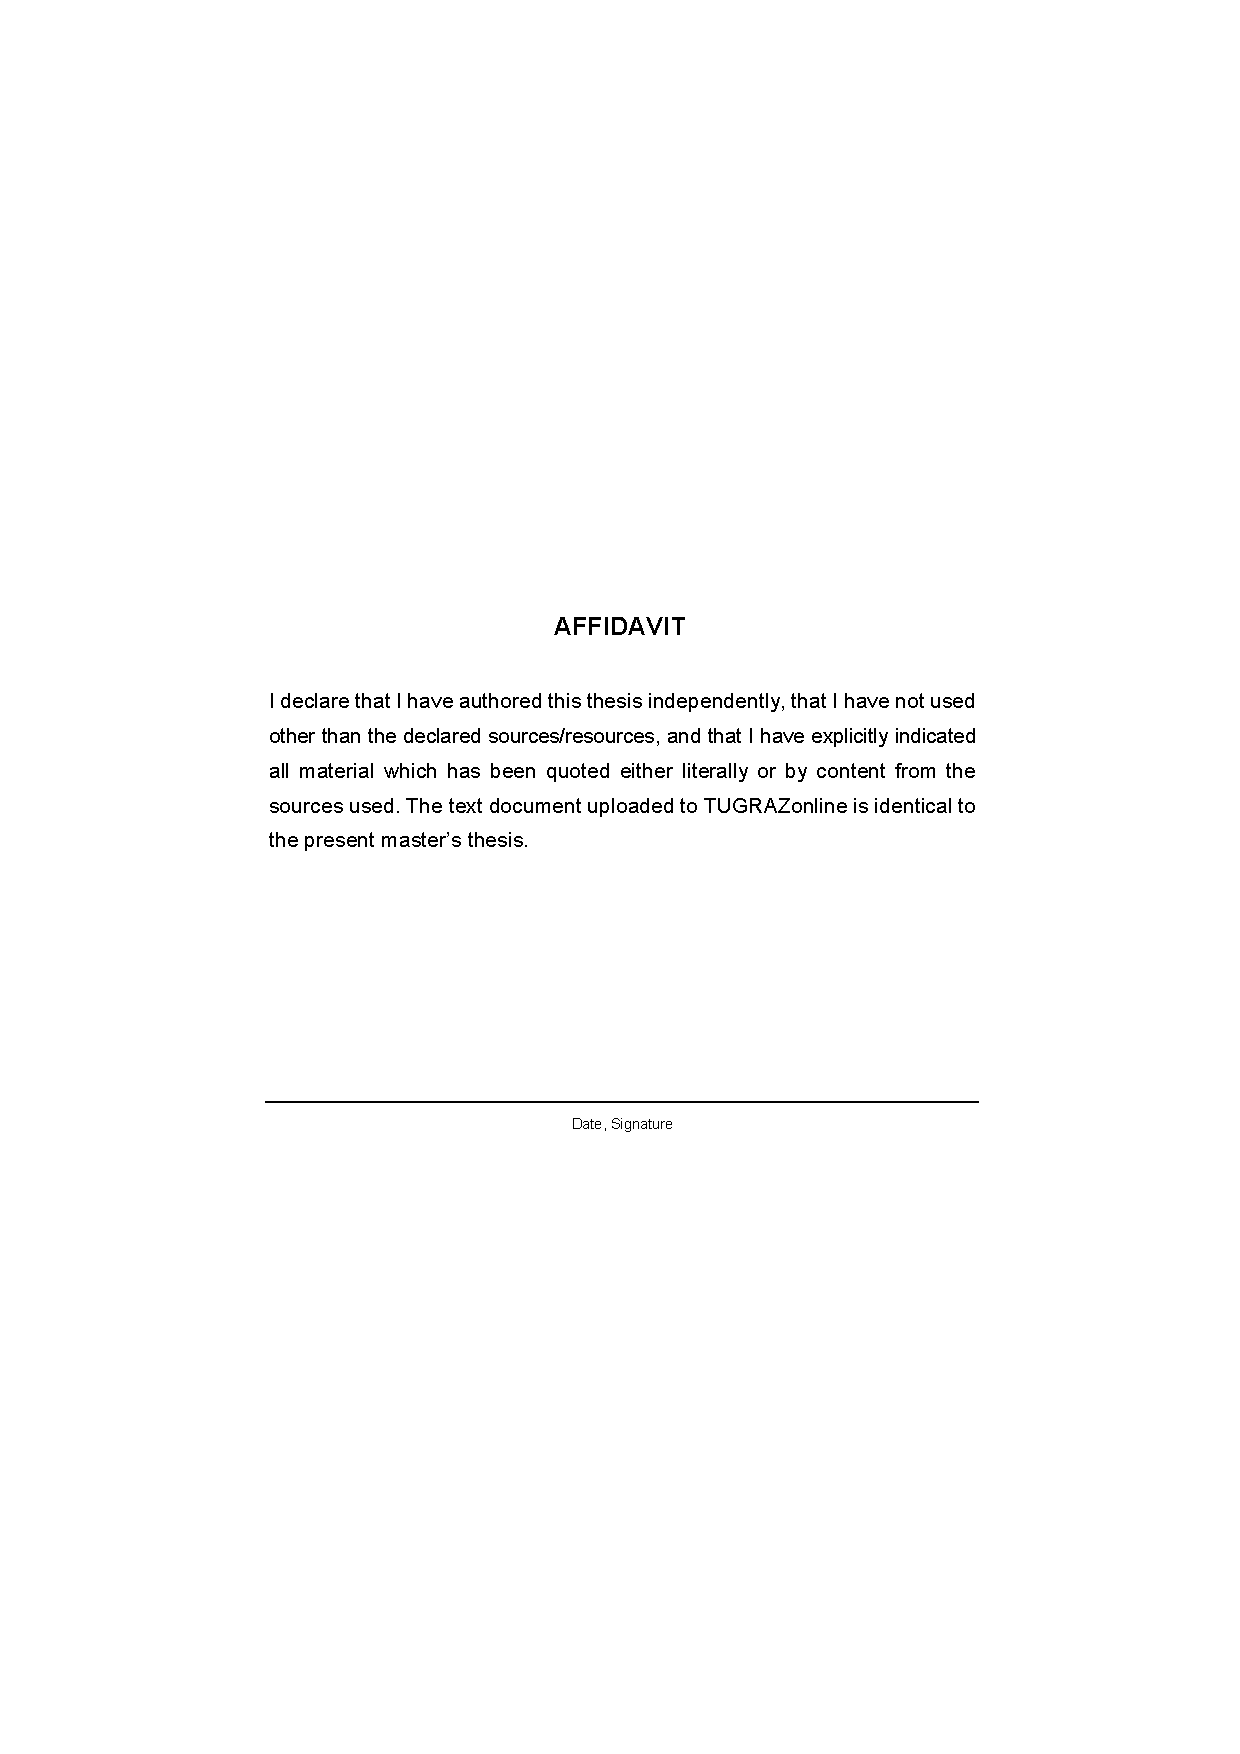
\includepdf[pages=-]{Affidavit.pdf}

\chapter*{Abstract}
The transient absorption microscope (TAM) is extended to probe higher energy states of squaraines, in this case squaraines with isobutyl sidechains abbreviated SQIB. No further states were found beyond the known ESA states, at probe \SIlist{440;500}{\nano\meter} for  pump 653 nm, when probing down to 300 nm, however peak positions by Zheng et. al\cite{Zheng2020} are reproduced qualitatively. The peak-shape has been observed slightly differently from Zheng. 

The extension of the probe capability is done by second harmonic generation of the optical parametric amplifier output for a resulting range of \SIrange{250}{470}{\nano\meter}. To avoid any fundamental wavelength influence, which tends to have a far higher responsivity on the detector, a prism is introduced to remove it ahead of the detector. Adjustments have to be made to the existing TAM setup to allow these higher photon energies, as the achromatic objectives of the existing setup are not rated beyond \qty{350}{\nano\meter} or \qty{3.54}{\electronvolt}. A switch to plano-convex UV-fused-silica (UVFS) lenses was required, which introduced the task of compensating and working with chromatic aberration of UVFS. New procedures to deal with the chromatic aberration are introduced and qualified. The procedures include a modification of the current alignment system by imaging the sample plane with another camera and introduction of a correction factor accounting for the spatial intensity distributions of pump and probe beam.

\chapter*{Kurzfassung}
Das Mikroskop zur Messung von transienten Absorptionsverläufen in Abhängigkeit von Anregungs- und Untersuchungswellenlänge bzw. Probe-Wellenlänge wird für höher energetische Wellenlängenbereiche erweitert um Squaraine Proben weiter zu charakterisieren. In dieser Arbeit wird SQIB, Squarainen mit Isobutyl Seitenketten, isotrop gelöst bearrbeitet. Es konnten keine weiteren ESA Verläufe bei höheren Photonenenergien als bereits zuvor bekannt beobachtet werden. Die bekannten transienten Absorptionspeaks bei zirka \SIlist{440;500}{\nano\meter} wurden qualitativ wie bei Zheng et al.\cite{Zheng2020}, wobei der Absorptionsverlauf etwas anders beobachtet wurde.

Die Erweiterung für höhere Photonenenergien wird durch Generation der zweiten Harmonischen (SHG) des Probes aus dem NOPA Ausgang bewerkstelligt, was Wellenlängen bis zu \qty{250}{\nano\meter} erreichen lässt. Um Einflüsse der fundamentalen Wellenlänge, welche für SHG verwendet wird, zu verhindern wird ein für UV transparentes Prisma vor dem Detektor verwendet. Grund ist die stark erhöhte Empfindlichkeit der Squaraine und des Detektors auf die typischen fundamentalen Wellenlängen gegenüber der verringerten Empfindlichkeit auf die gewünschten Wellenlängen im UV Bereich. Änderunge mussten bezüglich der Objektive gemacht werden, welche für die Fokussierung auf die Probe verwendet wurden. Grund ist reduzierte Transmission unter \qty{350}{\nano\meter} und eine fehlende Spezifikation für die Achromacität der Objektive für niedrigere Wellenlängen. Deshalb wurde auf UV-Quarzglas umgeschwenkt, welches jedoch stark wellenlängenabhängige Brennweiten besitzen, welche nun berücksichtigt werden mussten. Dafür werden deshalb neue Methoden um diese Wellenlängenabhängigkeit zu kompensieren eingeführt und getestet. Die neuen Methodiken beinhalten ein neuer Prozess zum Fokussieren auf die Probe mithilfe einer zweiten Kamera, welche in die Spiegelebene der Probe positioniert wird, und einem Korrekturfaktor der räumliche Intensitätsverläufe der beiden Strahlen in der Probe korrigiert.
\chapter*{Acknowledgements}
I would like to thank my colleagues at TU Graz and specifically at the Koch group at the institute of experimental physics for all their help. Things always turned out to be more complicated than at first expected and getting to this point would have been impossible without their help and feedback. Their endless patience and calm was certainly needed at times.

Specifically I would like to thank Robert Schwarzl for his assistance and time, as well as access to the TAM setup which essentially is the basis of his PhD. Working together on whatever may come up with such a setup was essential and without his support on everything would have been an insurmountable task.

My supervisor Markus Koch I would like to thank for this opportunity and his time....

I would also like to specifically thank Michael Stadlhofer and Florian Lindner for their time and patience in supporting me when Robert was doing research in the US. You both kept morals high and helped quickly whenever progress was stalled.

Thank Patricia, Simon Malacek and everyone IEP in general.

Finally I would like to thank my parents and family for supporting me all this time. I know it has not always been easy supporting my whims and I am deeply grateful for the unending support. Without you I would not have made it here.

\tableofcontents


\chapter{Prerequisites}

\section{Transient pump probe spectroscopy}
Using two short laser pulses the response of the sample to excitation is measured. The excited states generally have, depending on the process of their relaxation, lifetimes of femtoseconds to nanoseconds. To be able to observe charge transfer between molecules and other fast relaxation pathways femtosecond time resolution pulses are needed. The response to excitation is observed as a change in optical density. Time resolution of this transient process comes from shifting the point in time where one of the pulses passes the sample relative to the other, which is usually done by a simple path length change of one of the pulses.\newline
The measurement of transient absorption is based on the following: First a probe pulse of photon flux within a wavelength range passes through the sample and the remaining intensity is detected as $I_\text{probe}(\lambda_\text{probe})$. 
Secondly, after a period of time to allow the sample to relax back to its initial state, a pump pulse $\mathrm{I_{pump}(\lambda_{pump})}$ excites a volume of the sample. This leads to a direct change of the wavelength dependent optical density of the excited sample volume, which alters the transmission of the following probe photons $I_\text{pump-probe}(\lambda_\text{probe}, \lambda_\text{pump}, \Delta t) = I_\text{probe\, only}+\Delta I_\text{pump-probe}$, depending on the time delay $\Delta t$ between the pulses passing the sample volume and the pump and probe wavelengths $\lambda_\text{pump}/\lambda_\text{probe}$ respectively. \\
The initial change in absorption properties of the sample, depending on the pump pulse, is characterised in the transient absorbance $\Delta A$, which is often specified in orders of magnitude of the optical density $\left[\Delta A\right] = 1\, \text{OD}$. It is defined as seen in eq. \ref{eq:TA}.
\begin{equation}\label{eq:TA}
\begin{split}
\Delta A(\lambda_{\mathrm{pump}}, \lambda_{\mathrm{probe}}, \Delta t)&=-\log _{10}\left(\frac{I_{\mathrm{pump}-\mathrm{probe}}\left(\lambda_{\mathrm{pump}}, \lambda_{\mathrm{probe}}, \Delta t\right)}{I_{\mathrm{probe}}\left(\lambda_{\mathrm{probe}}\right)}\right)\\
&=-\log _{10}\left(1+\frac{\Delta I_{\mathrm{probe}}\left(\lambda_{\mathrm{pump}}, \lambda_{\mathrm{probe}}, \Delta t\right)}{I_{\mathrm{probe}}\left(\lambda_{\mathrm{probe}}\right)}\right)
\end{split}
\end{equation}

\section{Transient effects in pump probe spectroscopy}
There are several types of contrast in pump-probe transient spectroscopy. Processes like two-photon-fluorescence, second or third harmonic generation require power densities too high for our samples and would lead to quick deactivation. They are thus not going to be addressed further with respect to the sample transient processes. The most relevant ones for this experimental setup are:\cite{Zhu2020}
\begin{itemize}
\item Stimulated emission (SE): Possible in cases where a state, below or at the excited level, has a transition to a lower state corresponding to the temporally second pulse wavelength used. This could be either pump or probe exciting and then the other leading to stimulated emission. This can lead to contrast for either pump or probe wavelengths, when not using a wavelength dispersive detector setup. For pump contrast it would manifest as a rise in transmission towards temporal overlap, when the probe passes the sample first, and a sharp falloff at temporal overlap. For probe contrast the behaviour would be like for GSD.
\item Ground state depletion (GSD): By moving part of the ground state population to different energy levels the probe pulse sees a smaller absorption cross-section. This is seen as a positive change in transmission ($\Delta A < 0$). The signal returns by an \text{(multi-)exponential} decay to the initial transmission behaviour, as the molecules relax back to the ground state. Multi exponential decays are expected in general if there are multiple states excited.
\item Excited state absorption (ESA): Similar to GSD a population transfer from the ground state happens, however with this population transfer now a state previously not accessible with the probe pulse becomes accessible, thus leading to an increase in absorption ($\Delta A > 0$) and a reduction of transmission.
\item Photothermal effect: Due to heating from strong absorption of the pump beam a change in the refractive index changes the propagation path of the probe beam. It can be avoided by having a larger numerical aperture in the rear focusing element than for the front focusing element, to ensure all light is still collected, or by changing repetition frequency.
\item Cross phase modulation (XPM): Through the optical Kerr effect the refractive index changes when both pump and probe beam are temporally overlapped within the sample. This may be used to check the instrument response of the transient absorption microscope. It can be avoided, like the photothermal effect, by a larger condenser numerical aperture.
\item Stimulated raman scattering: In case the energy difference between pump and probe corresponds to a raman active state a photon transfer from the higher energy beam to the lower energy beam may happen. For this process there needs to be temporal overlap of the beams. This is a $\chi^{\left(3\right)}$ process that is unlikely to be observed in our sample at irradiances used.\cite{Prince2017}
\end{itemize}

These processes may manifest at the same time, thus concealing other processes with the opposite influence on the transient absorbance. This is not so much of concern for processes like XPM or stimulated raman scattering, because they require temporal overlap of pump and probe pulse and thus only influence a short range within the time delay range based on the pulse lengths. ESA and GSD are measured within a power-regime linear to the pump irradiance of the sample, where the peak power of the pulse is not high enough for nonlinear optical processes. For this reason the temporal pulse shape is not so important for the classification of these measurements, other than time resolution. Thus it makes sense to write powers used for pump and probe as dose per area per shot (\SI{1}{\radExp}) or radiant exposure per laser shot $\mathrm{H}_{x_0,y_0}$, to also avoid confusing quantities due to different repetition rates of pump and probe pulses. $\mathrm{H}_{x_0,y_0}$ refers to the radiant exposure at the center of the fitted Gaussian point spread function.\\

To record a GSD spectrum simply an excitation from the groundstate (GS) has to be available for the probe beam spectrum as seen in fig. \ref{fig:probeOnly}. ESA needs a state reachable from the pumped state with the probe spectrum, as seen in fig. \ref{fig:probeAfterPump}. The available photon wavelengths for pump and probe may be seen in tab. \ref{tab:NOPAs}. An important factor is that neither pump or probe are mono-energetic light and they will excite off center wavelengths.

\begin{figure}[hbtp]
\centering
\begin{subfigure}[t]{0.3\textwidth}
\centering
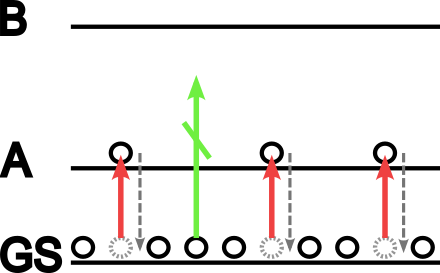
\includegraphics[width=\linewidth]{images/TA-explanationProbeOnly.png}
\caption{Probing of sample in groundstate at $t-t_\text{sample\, pump} < 0$ at two different photon energies.\label{fig:probeOnly}}
\end{subfigure}
\hfill
\begin{subfigure}[t]{0.3\textwidth}
\centering
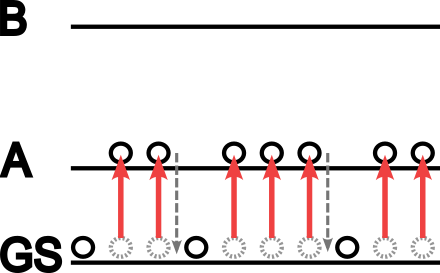
\includegraphics[width=\linewidth]{images/TA-explanationPumpOnly.png}
\caption{Pumping of sample in ground state}
\end{subfigure}
\hfill
\begin{subfigure}[t]{0.3\textwidth}
\centering
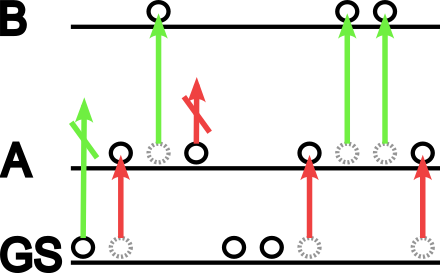
\includegraphics[width=\linewidth]{images/TA-explanation-probe-after-pump.png}
\caption{Probing of sample  after pump at $t-t_\text{sample\, pump} > 0$ at two different photon energies. \textcolor{green}{Green} experiences ESA and \textcolor{red}{red} experiences GSD.\label{fig:probeAfterPump}}
\end{subfigure}
\caption[Principle of pump probe spectroscopy with excited states absorption and ground state depletion.]{Principle of pump probe spectroscopy with ESA and GSD. GS is the groundstate of the sample without excitation. A is a low energy state that may be excited from GS. B is a higher energy excited state that may be populated from both GS and A. Fig. \ref{fig:probeOnly} shows the probe passing the sample at a time where no excitation has happened yet. This is the case both for the reference probe only measurement as well as for the pump-probe measurement ahead of temporal overlap. $t_\text{sample\, pump}$ refers to the time where the pump pulse is passing the sample.\label{fig:CompendiumTA}}
\end{figure}

\subsubsection{Delay scan in detail}
A single measurement point usually consists of multiple delay scans averaged together, for which an example is shown in fig. \ref{fig:exampleDelayScans}. The relative absorbance signal of a delay scan should consist of:
\begin{enumerate}
\item Background plateau, where the probe pulse passes the sample in time ahead of the pump pulse.
\item Rising signal edge, that may be positive or negative, depends on the instrument response time (pulse lengths) as well as the number of delay points measured.
\item Maximum signal response, where transient processes that require temporal overlap tend to be observed.
\item Signal decay without temporal overlap of the pulses, where the sample relaxes from the excited state. This may include energy transfer processes to other molecules, if the sample and the environment are suitable.
\end{enumerate}
The background plateau is simply used to subtract any non probe signal detected, such as stray pump light or sample fluorescence. This also serves as an indicator of lateral pump movement with stage movement, which can be problematic depending on the alignment of pump and probe. If it is a slow change regarding delay setting it may be subtracted linearly.\\
Rising signal edge follows an error-function of the pump pulse, as femtosecond pulses usually have a Gaussian temporal shape which cumulatively excites the sample for the probe pulse to detect. This rise allows for an estimate of the temporal pulse length and instrument response.

\begin{figure}[hbtp]
\centering
\begin{subfigure}[t]{\textwidth}
\centering
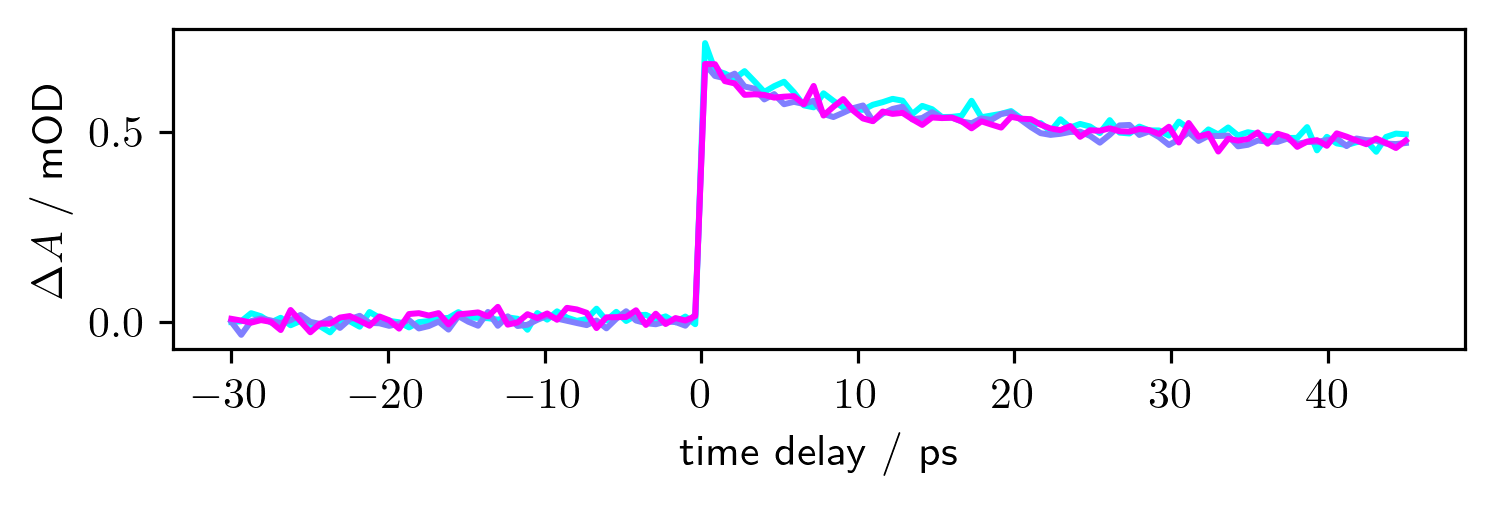
\includegraphics[scale=1]{images/TA_delayscan_493RAW.png}
\caption{Pump \SI{653}{\nano\meter} probe \SI{493}{\nano\meter} ESA TA\_fourier 6767-6769}
\end{subfigure}
\begin{subfigure}[t]{\textwidth}
\centering
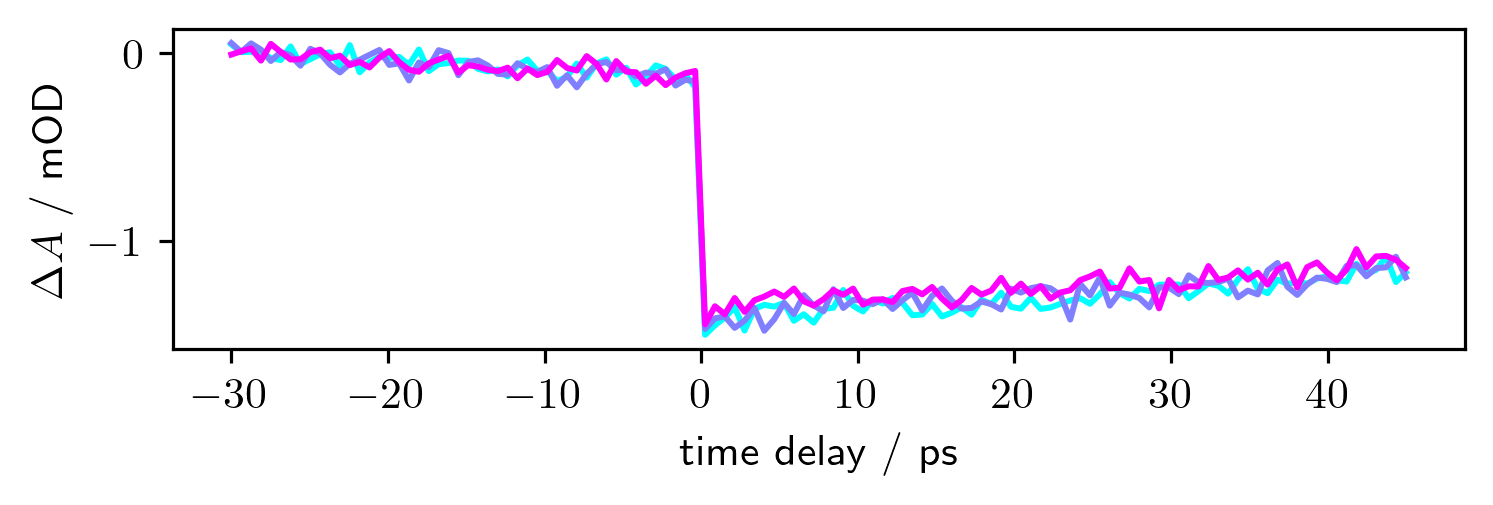
\includegraphics[scale=1]{images/TA_delayscan_680RAW.png}
\caption{Pump \SI{653}{\nano\meter} probe \SI{680}{\nano\meter} GSD TA\_fourier 6677-6679}
\end{subfigure}
\caption[Exemplary excited state absorption and ground state depletion measurement series of 1wt\% SQIB in PMMA]{Examples of measurement series featuring ESA or GSD for 1wt\% SQIB in PMMA. Raw measurements without any correction are shown. Each curve is a single measurement belonging to the series plotted in the corresponding figure. Measurements are done successively, thus the delay range is scanned for each of the scans.\label{fig:exampleDelayScans}}
\end{figure}


\subsection{Polarization angles}\label{sec:PolAngles}
Depending on molecular geometry or crystal geometry transition dipole moments may have different orientations, which may be resolved by different polarisations of pump and probe pulse. On the other hand, when working with liquids or molecule-environment combinations with strong relaxation effects upon excitation, the orientation of the transition dipole moments may rotate, relative to where they would be in their zero time direction. This leads to a measurable signal change over time, which may be characterised by the anisotropy:\cite[chapter 10]{Lakowicz2008}
\begin{equation*}
r = \frac{I_{\parallel}-I_{\perp}}{I_{\parallel}+2I_{\perp}}
\end{equation*}
where $I_\parallel$ is the component with pump and probe parallel polarizations, and $I_\perp$ is the component with probe perpendicular to the pump polarization. The anisotropy at pump excitation time is given by the Perrin-formula $r\, =\, \frac{1}{5}\left(3\mathrm{cos^2}\beta-1\right)$, which gives a maximum anisotropy of $r=0.4$ for parallel pump and probe. Note that the formula does not apply to multi-photon pump or probe processes.  By measuring at the so called "magic angle" of $\theta = 54.7 \degree$ the parallel and orthogonal polarization components are equalised geometrically and the measurement is made isotropic. This is based on the transmission of polarized light through a polariser $I(\theta) = I_0 \mathrm{cos}^2(\theta)$. \cite[chapter 10]{Lakowicz2008}\cite{Schalk2010}\\
Alternatively this isotropic output may also be achieved by measuring parallel and orthogonal polarisations and using an arithmetic correction. The total intensity is $I_\text{T} = I_x+I_y+I_z = 2\cdot I_\perp + I_\parallel$. The reason for the factor 2 is that the original polarization can rotate into two perpendicular directions, which are projected into a direction perpendicular to the pump polarization. One of these is parallel to the propagation direction of the probe however and may not be measured. To now account for both orthogonal rotation directions, the signal may be corrected to $I = \frac{I_\parallel + 2I_\perp}{3}$, which corresponds to the isotropic signal.\cite{Zheng2020}



\section{Squaraines}
\begin{figure}[hbtp]
\centering
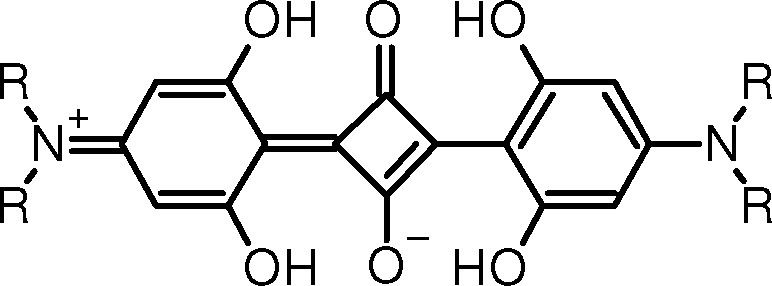
\includegraphics[width=0.6\linewidth]{images/nAlinoSquaraine.jpeg}
\caption[Chemical structure of anilino squaraine.]{Chemical structure of anilino squaraine used within this thesis. Side chains R are iso-butyl.\label{fig:chemStructureSQIB}}
\end{figure}

Squaraines are investigated for multiple properties making them an interesting model system for organic solar cells. Processing for prototyping is very simple and may be done by spin-coating, like the samples provided by Manuela Schiek.

For crystalline squaraines the stacking and geometry of the unit cell may be tuned by choosing side-chain molecules of appropriate bulkiness. A wide choice of alkyl chain lengths from butyl to octyl, isobutyl and similar molecules that do not directly influence the monomer spectrum are available. \cite{Hestand2015, Brueck2014, Balzer2022} 

Theoretical modelling may be done with the semi-empirical essential states model, simplifying the large molecules to a donor-acceptor-donor structure, where the central oxygen groups with high electron affinity act as the acceptors and the nitrogens in the periphery of the molecule as donors. Opposed to the Frenkel excition model the essential states model allows states to diabatically mix to account for changes in charge distribution due to intermolecular and solvent interactions. This is needed due to the highly polarisable nature of the molecules. This works well to reproduce features such as davydov splitting, which is an effect for unit-cells with more than one molecule or multiple molecular sub-units with interacting transition dipole moments.\cite{Zhong2019, Hestand2015} 



\begin{figure}[hbtp]
\centering
\begin{subfigure}[b]{\textwidth}
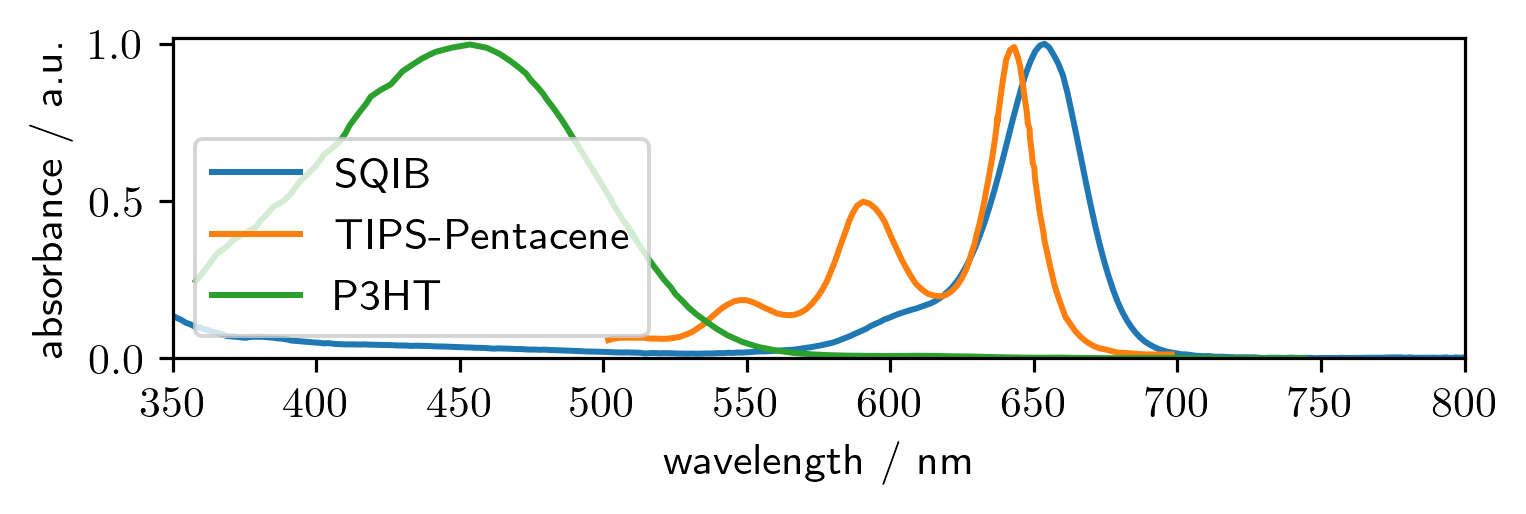
\includegraphics[width = \textwidth]{images/spectra/OSC/ComparisonOfOSCSolution.png}
\caption{Comparison of individually normalised absorbance spectra of organic semiconductors in solution. Preliminary CW transmission spectrum of the 1wt\% SQIB in PMMA by Manuela Schiek 2022.\cite{Schiek2022} TIPS-Pentacene in toluene solution.\cite{Schaberle2020} P3HT in 3-hexylthiophene solution\cite{Rahimi2014}.}
\end{subfigure}
\begin{subfigure}[b]{\textwidth}
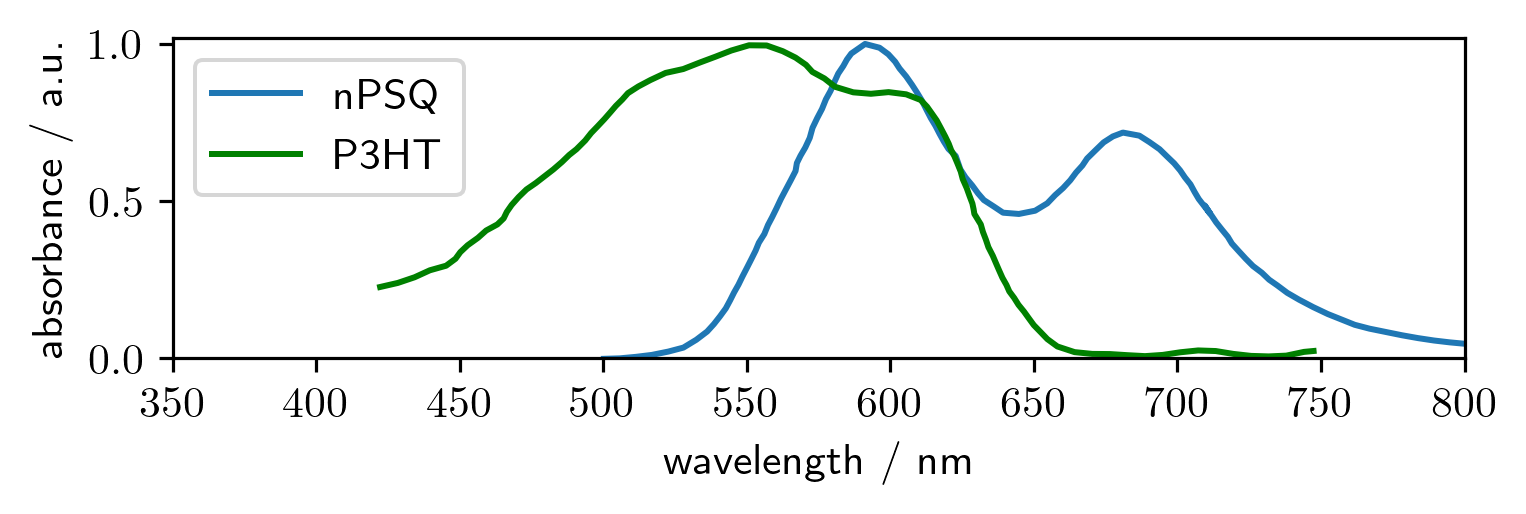
\includegraphics[width = \textwidth]{images/spectra/OSC/ComparisonOfOSCCrystal.png}
\caption{Comparison of annealed polycrystalline nPSQ\cite{Balzer2022} and spin cast thin film P3HT absorbance spectra. Note that P3HT is a polymer chain, which may exhibit amorphous regions when spin cast.\cite{Rahimi2014}\label{fig:crystOSC}}
\end{subfigure}
\caption[Comparison of organic semiconductor absorption spectra.]{Comparison of organic semiconductor absorption spectra. External data digitised for plotting with WebPlotDigitizer.\cite{Rohatgi2022}\label{fig:compOSC}}
\end{figure}

\begin{figure}[hbtp]
\centering
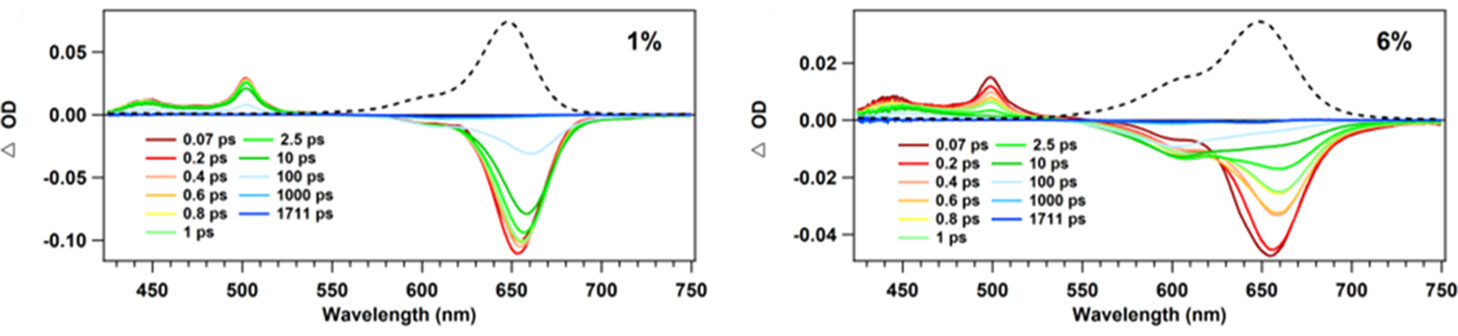
\includegraphics[scale=1.2]{images/Zheng2020SquaraineTAgraphCut.jpeg}
\caption[Transient absorption spectra of squaraine with n-butyl sidechains by Zheng.\cite{Zheng2020}]{Transient absorption spectra of squaraine with n-butyl sidechains.\\
Reprinted and adapted with permission from \protect\bibentry{Zheng2020}. \\Copyright 2020 American Chemical Society\label{fig:zhengTA}}
\end{figure}

A comparison of absorption behaviour of other organic semiconductors is made in fig. \ref{fig:compOSC}, where P3HT is a polymer semiconductor that is also researched for use in organic solar cells.\cite{Holliday2016} TIPS-Pentacene on the other hand is mainly researched for use in organic thin film transistors, but also for singlet triplet fission in organic solar cells.\cite{Schaberle2020} The double peak for nPSQ, a similar squaraine sharing the same monomer spectrum with different sidechains, in fig. \ref{fig:crystOSC} is an attribute of the above mentioned Davydov splitting, due to multiple molecules within the unit cell.\cite{Balzer2022} Additionally transient absorption spectra for similar squaraines, with n-butyl side-chains, are already available for comparison, see fig. \ref{fig:zhengTA}.\cite{Zheng2020}



\chapter{Devices and Setup}

Part of the experimental objective was to extend the range of the transient absorption microscope (TAM) into the UV range via SHG of the probe NOPA output. With the extension a wavelength range of 250 nm to 940 nm, with a gap between 470 nm and 500 nm, is available for probing the sample. To achieve this range a few optics, most notably the achromatic objectives used to image the sample, had to be exchanged for optics transparent in the UV.
\section{Regular transient absorption microscope setup}\label{RegTAM}
A short description of the experimental setup for the transient absorption microscope (TAM), as it was before attempting an extension to higher photon energies, follows:\newline
As a laser source a PHAROS, Yb based, femtosecond laser by Light Conversion is used with an output of 400 µJ at 40 kHz, at a pulse length in the range of 270 fs. The output is evenly split between two Orpheus Non-Collinear Optical Parametric Amplifiers (NOPAs), where one is setup with second harmonic (2H) of the Yb-based pump laser (514 nm) for the pump pulses and the other is setup with third harmonic (3H) of Yb (342 nm) for the probe pulses. Some of the NOPA specifications are shown in tab. \ref{tab:NOPAs}. Output power stability is mainly important for the pump pulse, which is why the setup, including the pulse compressor of PHAROS, is optimized for maximum stability of the 2H NOPA. Having low shot to shot fluctuations is important in all cases. PHAROS is the most reliable part of the setup. The PHAROS compression setting may need adjusting every few months. For further details see previous work by Schwarzl et al.\cite{Schwarzl2022}\\

Output wavelengths of the NOPAs may deviate from the set wavelength, as they are set by parameter curves. The NOPAs settings have to be adjusted such that the centroid output, which is controlled via the internal Qmini spectrometer, is on the wavelength intended. The centroid is used, as the maximum intensity wavelength may be offset from the center of the pulse spectrum. Also note that as seen in fig. \ref{fig:spectrometerMalfunction} the spectrometer data may show periodic intensity variations, which are a device malfunction. Using the centroid avoids strong interference by this type of malfunction. In case of low output power resetting motors multiple times may suffice.

\begin{table}
\caption[Specifications of NOPAs used together with the Light Conversion PHAROS to pump and probe the sample.]{Specifications of NOPAs used together with the Light Conversion PHAROS to pump and probe the sample. Temporal envelope values date from commissioning of the setup. Setup currently is tuned for 2H power stability, which is used to supply the pump pulse. Temporal envelopes of SHG signal were not measured.\label{tab:NOPAs}}
\begin{tabular}{lccc}\toprule
Device configuration & wavelength range / nm & photon energy range / eV & temporal envelope / fs \\ \midrule
2H & \SIrange{650}{940}{} & \SIrange{1.32}{1.91}{} & $\leq$ 50 \\ 
2H-SHG & \SIrange{325}{470}{} & \SIrange{1.32}{1.91}{} & - \\\midrule
3H & \SIrange{495}{680}{} & \SIrange{1.82}{2.50}{} & $\leq$ 40 \\
& \SIrange{680}{900}{} & \SIrange{1.38}{1.82}{} & $\leq$ 90 \\
& \SIrange{900}{940}{} & \SIrange{1.32}{1.38}{} & $\leq$ 110 \\
3H-SHG& \SIrange{250}{470}{} & \SIrange{2.63}{4.96}{} & - \\ \bottomrule
\end{tabular}
\end{table}

\begin{figure}[hbtp]
\begin{subfigure}[b]{\textwidth}
\centering
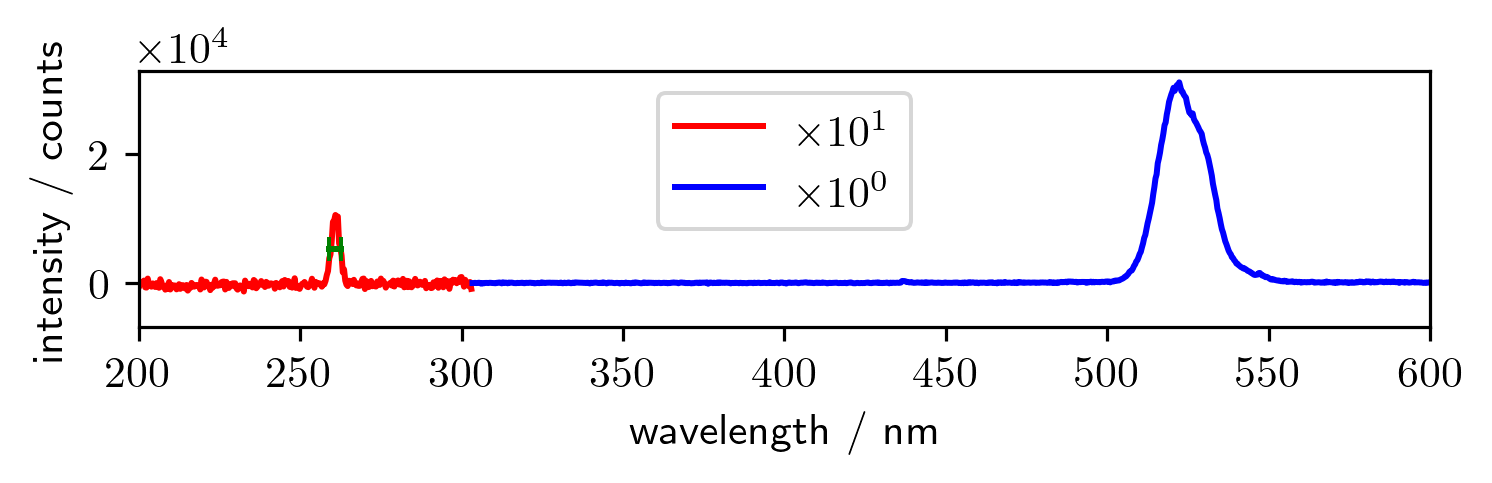
\includegraphics[scale=1]{images/spectra/SpectrumExampleNoFilter_260nm.png}
\caption{FWHM$_{\mathrm{SHG}}$ = \SI{3.9}{\nano\meter}, FWHM$_{\mathrm{fundamental}}$ = \SI{18.9}{\nano\meter} FLAME-S spectrometer}
\end{subfigure}
\begin{subfigure}[b]{\textwidth}
\centering
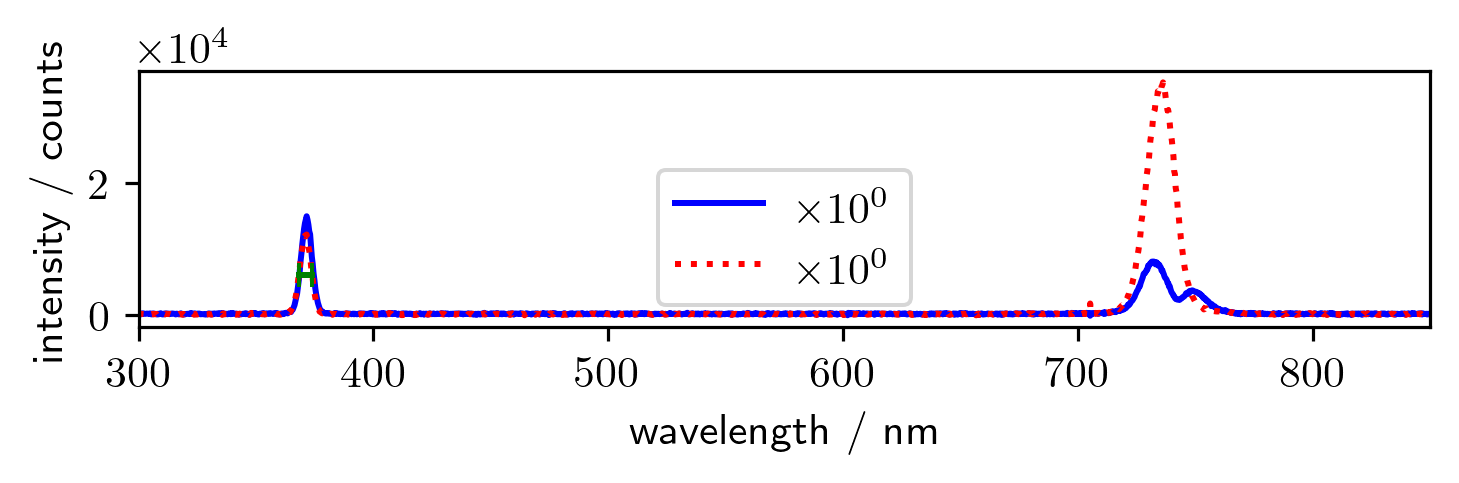
\includegraphics[scale=1]{images/spectra/SpectrumExampleNoFilter_371nm.png}
\caption{FWHM$_{\mathrm{SHG}}$ = \SI{5.6}{\nano\meter}, FWHM$_{\mathrm{fundamental}}$ = \SI{14.0}{\nano\meter}, Qmini internal spectrometer\label{fig:SHG_offCenterComp}}
\end{subfigure}
\begin{subfigure}[b]{\textwidth}
\centering
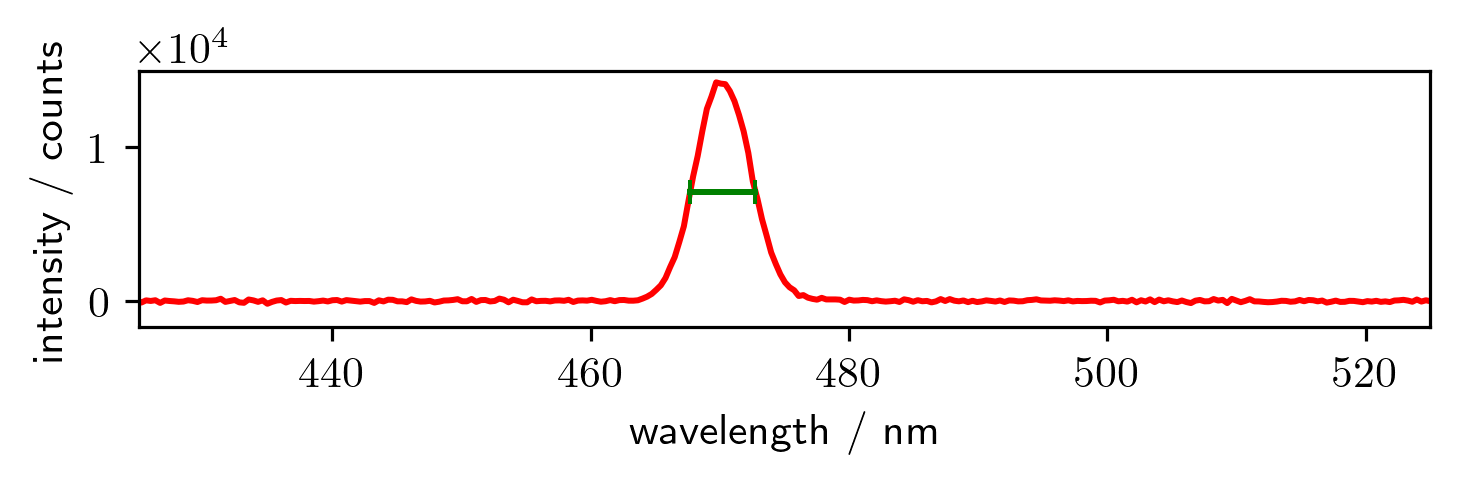
\includegraphics[scale=1]{images/spectra/SpectrumExampleNoFilter_470nm.png}
\caption{FWHM$_{\mathrm{SHG}}$ = \SI{5.1}{\nano\meter}, Qmini internal spectrometer}
\end{subfigure}
\begin{subfigure}[b]{\textwidth}
\centering
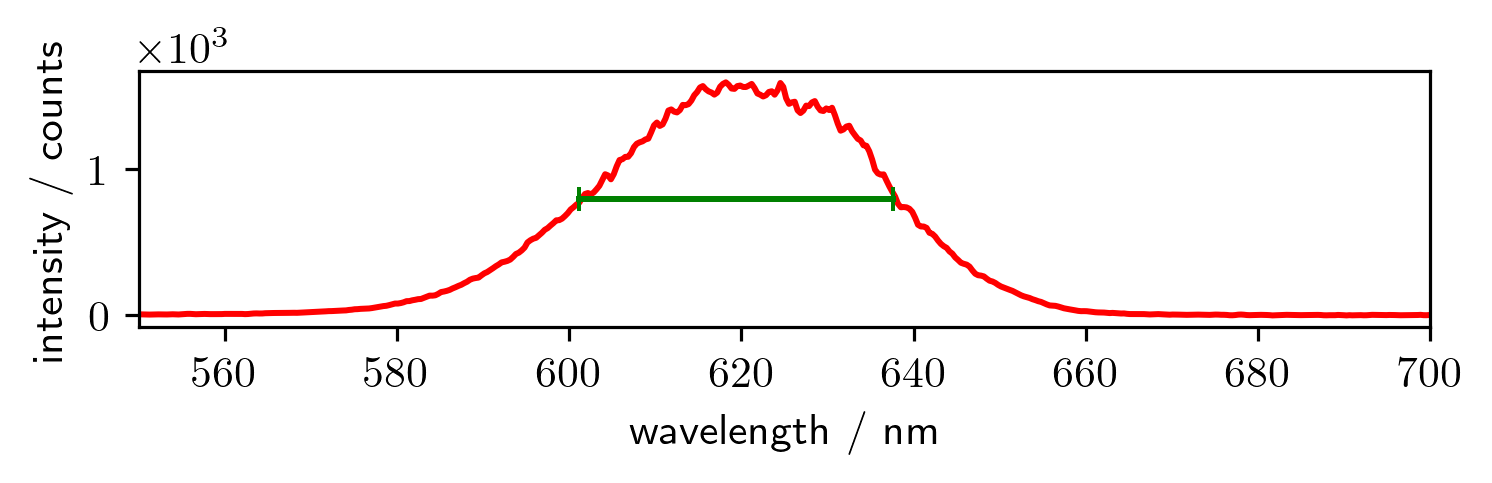
\includegraphics[scale=1]{images/spectra/ActonMonochromatorCharacterisation/620nmSpectrumProbe.png}
\caption{FWHM$_{\mathrm{NOPA}}$ = \SI{36.5}{\nano\meter}, Qmini internal spectrometer}
\end{subfigure}
\begin{subfigure}[b]{\textwidth}
\centering
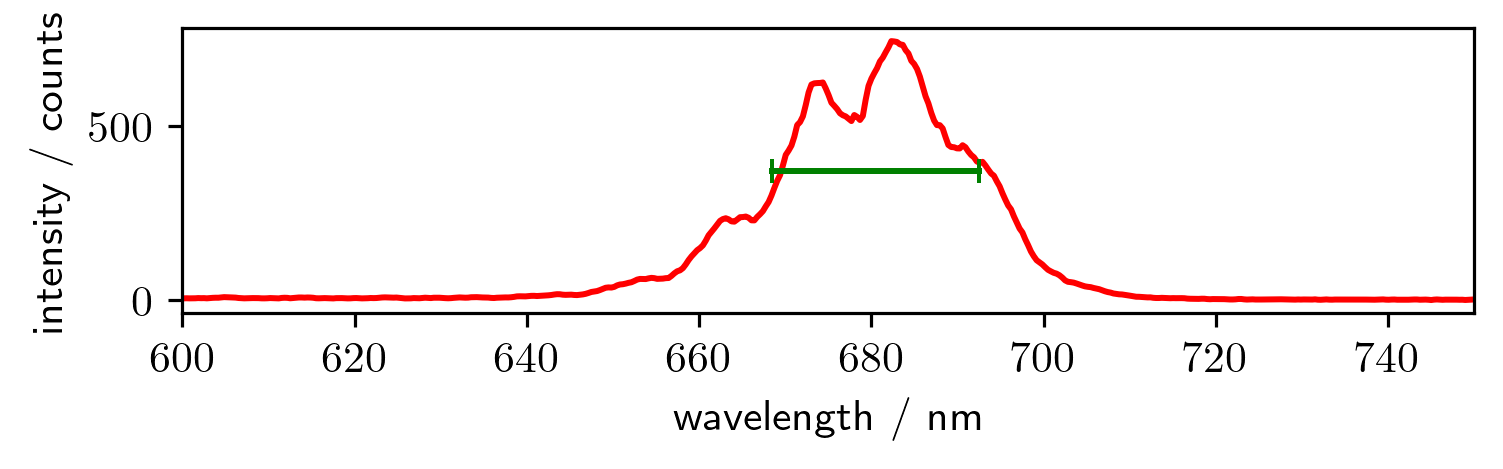
\includegraphics[scale=1]{images/spectra/2024-02-05/probe_3H_680nm.png}
\caption{FWHM$_{\mathrm{NOPA}}$ = \SI{24.1}{\nano\meter}, Qmini internal spectrometer; Spectrometer started modulating intensity as shown periodically. Modulation is consistent.\label{fig:spectrometerMalfunction}}
\end{subfigure}
\caption[Examples for spectra used to probe the sample.]{Examples for spectra used to probe the sample. FWHM is calculated with Waves software.\label{fig:probeSpectra}}
\end{figure}

\begin{figure}[hbt]
\centering
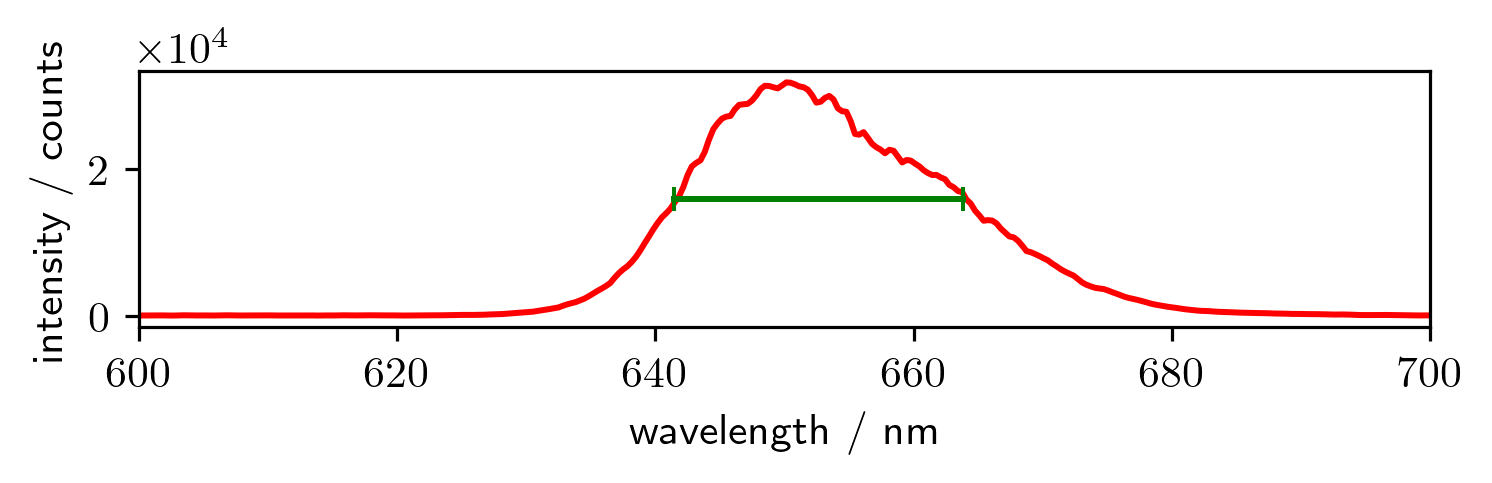
\includegraphics[scale=1]{images/spectra/2024-02-05/pump_2H_653nm.png}
\caption[Example of typical \qty{653}{\nano\meter} pump spectrum.]{Example of typical pump spectrum.\\ FWHM = \SI{22.4}{\nano\meter}, Qmini internal spectrometer; 653 nm pump as used for measurements. \label{fig:specRefPump}}
\end{figure}

The light following the pump path goes through several apertures and ND filters until the beam reaches the linear delay stage, which uses a Newport LTA-HS actuator.  Filters may be absorptive glass filters or metal coated reflective filters, including gradient filters for linear adjustability.  The beam path is then led through the chopper near the center focus of a  1:1 telescope. The chopper blocks every second pulse, leaving a half frequency signal for the pump. The chopper is synchronised to a signal output of PHAROS, which allows setting a binary on and off modulation of the pump pulses. After passing through a lambda half wave plate the beam enters the common path in the cage with the sample.

The probe beam has the same treatment of apertures and ND filters, including a variable reflective one, and goes through a $\mathrm{\lambda/2}$ plate until it reaches the common path.


For detection of the transient signal a custom made detector based on Hamamatsu S1336-8BK Si photodiode is used in combination with an analogue long pass amplification circuit stretching the signal such that it can be measured with a picoscope 5442D. For all measurements detector "A" was used. The diode is fit for measurements in the wavelength range of 190-1100 nm. The actual quantum efficiency change over the spectral range does not matter in detail, as the variation over the spectral range is slow and does not exceed 10\% of the spectral range of a probe setting at any point.

\section{UV extended transient absorption microscope setup}
This section will address the issues that emerged with the extended setup as well as attempted solutions and the final changes to make it work.

\begin{figure}[h]
\centering
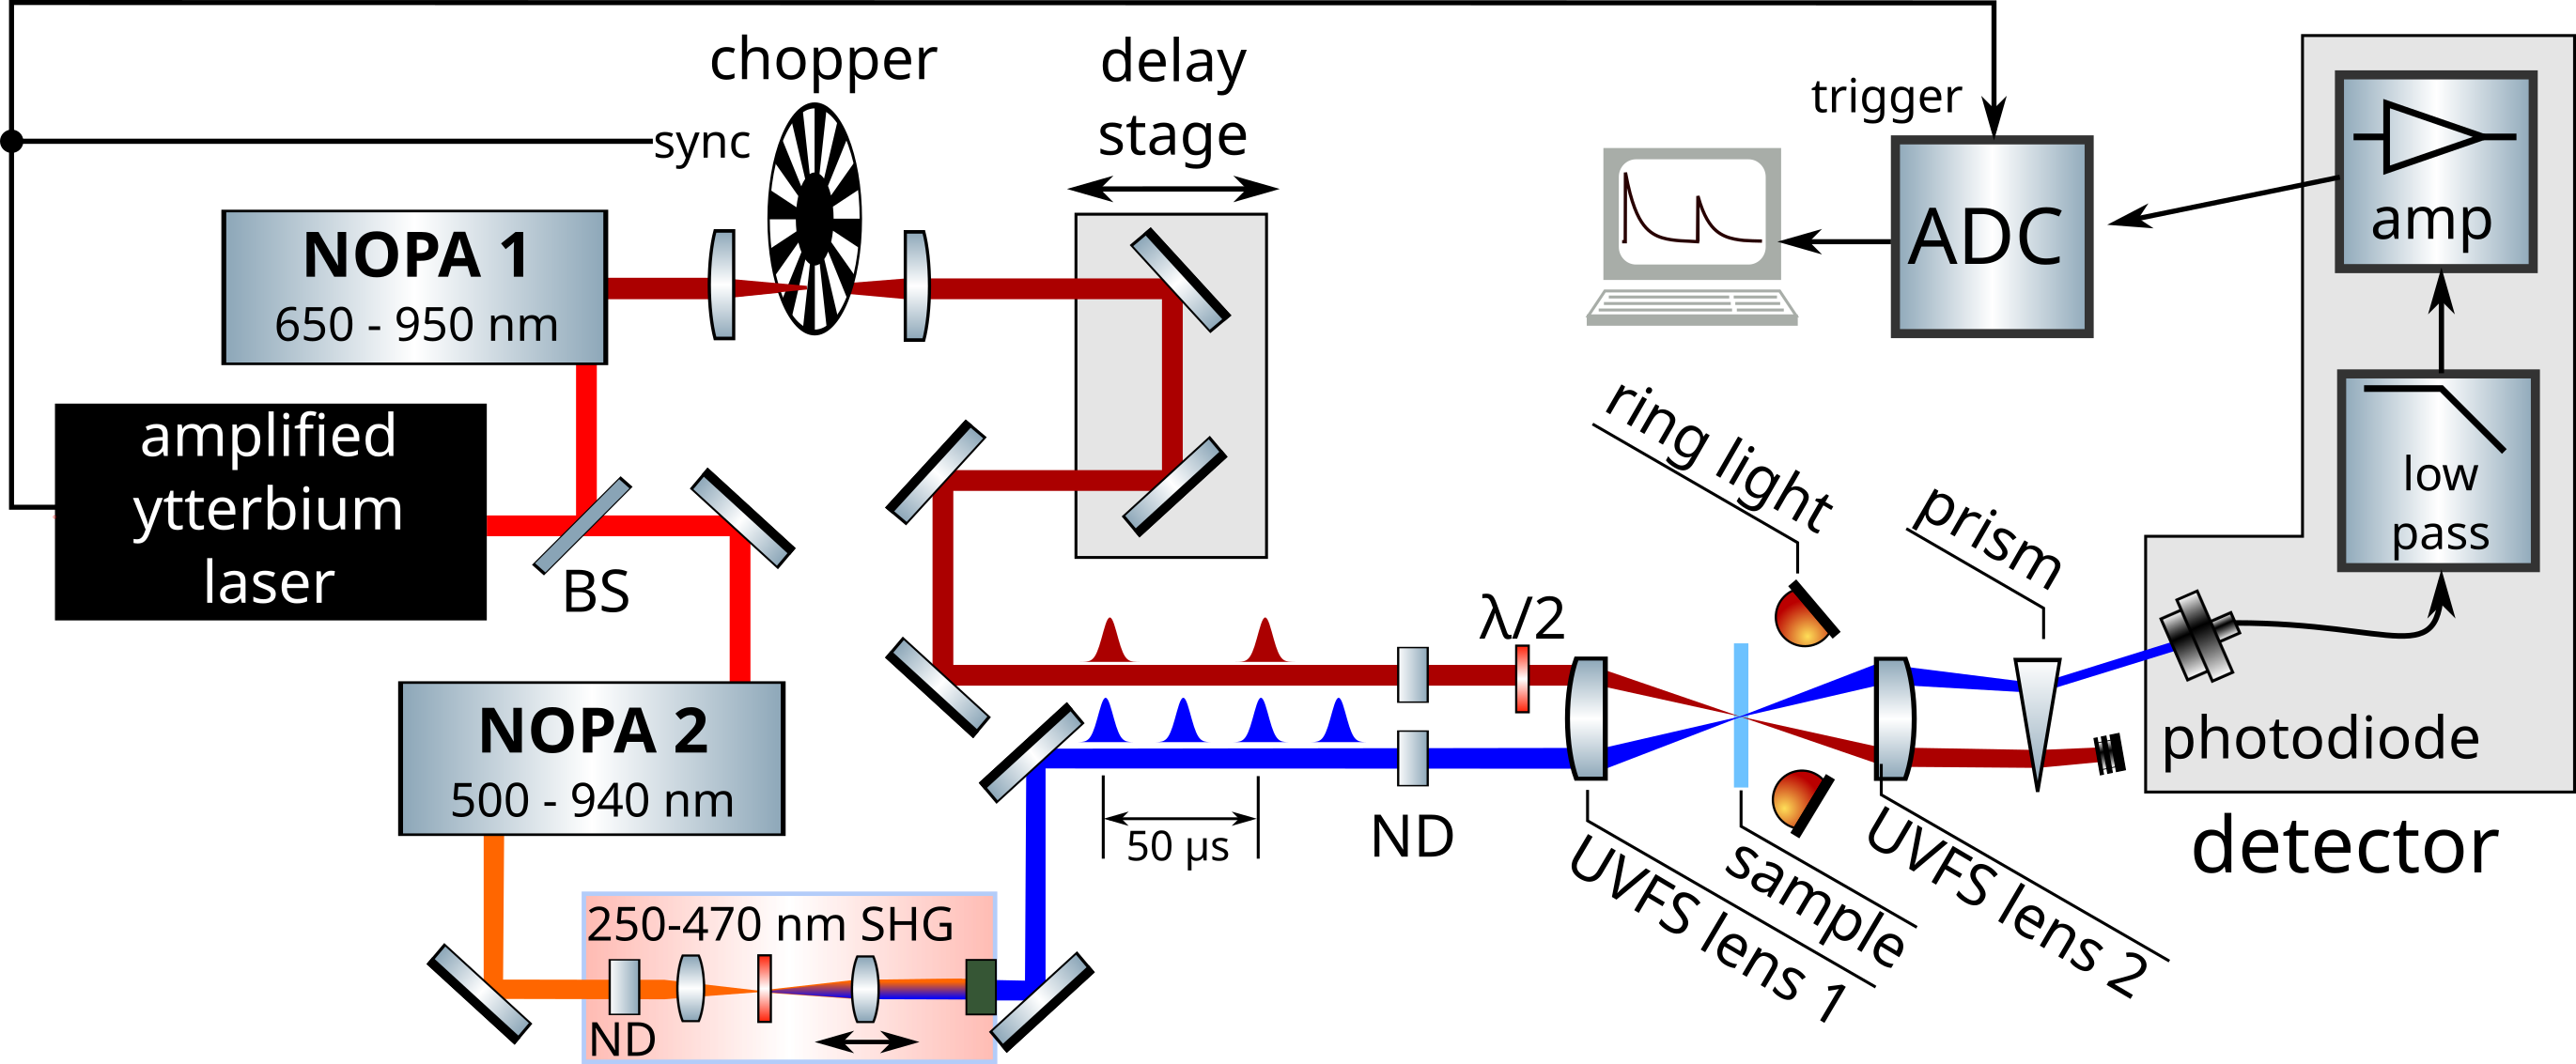
\includegraphics[width=0.9\linewidth]{images/ComponentLibrary_svg/experimental_tam_shg_swapped.png}
\caption[UV extended transient absorption microscope setup.]{UV extended transient absorption microscope setup. Available pump and probe settings in tab. \ref{tab:NOPAs}.
SHG stage shown including optional filter fundamental wavelength of SHG (after SHG crystal). Filter to remove the white light background of the 3H NOPA may be inserted ahead of the SHG stage. Cage setup in further detail in fig. \ref{fig:CageSetup}. Created with component library.\protect{\cite{Franzen2006}}}
\end{figure}

\begin{figure}[h]
\centering
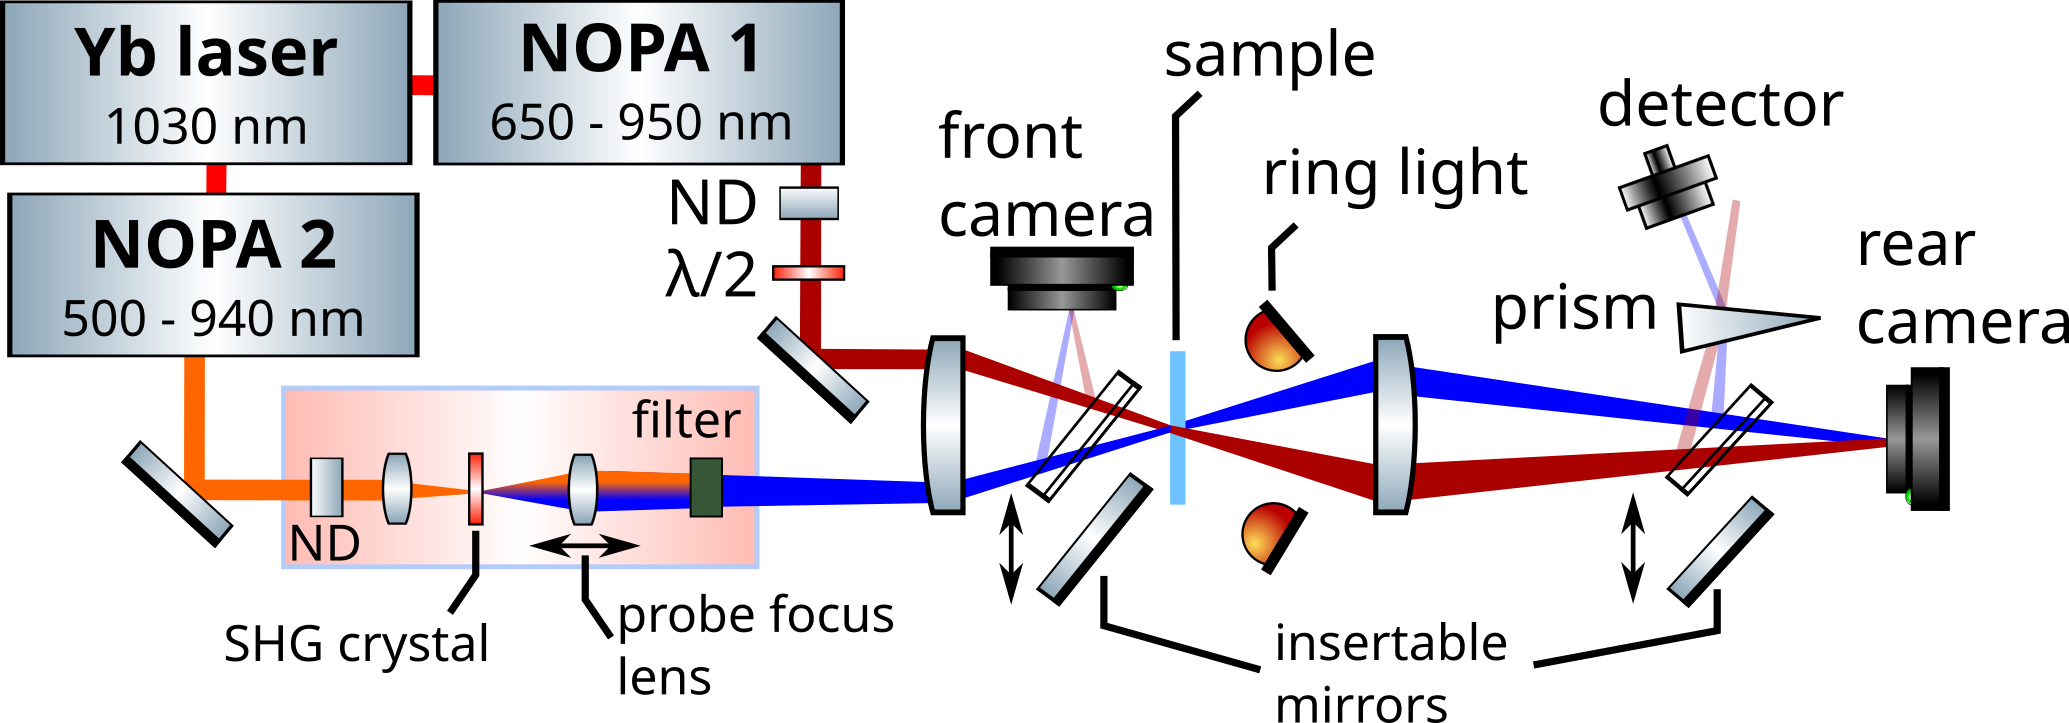
\includegraphics[width=0.9\linewidth]{images/ComponentLibrary_svg/SHG-focusing-large.png}
\caption[Detail view of new components in the transient absorption microscope.]{Detail view of new components in TAM. Ahead of first SHG probe lens white light remainder from NOPA may be filtered and after the second lens the fundamental may be filtered. Created with component library.\protect{\cite{Franzen2006}}\label{fig:CageSetup}}
\end{figure}

\subsection{Cage setup}\label{sec:cageSetup}
To accommodate wavelengths below \qty{350}{\nano\meter} the objectives have to be exchanged, as absorption reduces the transmission of the objective combination severely. Furthermore only one of the objectives is rated down to 350 nm, raising the question if their achromacity still is a viable assumption.\newline
The objectives are replaced with  uncoated 125 nm plano-convex UV fused silica (UVFS) lenses from EKSMA (110-1216ET), with the convex side placed such that the collimated beam enters or exits the convex side. This means that the planar sides of the lenses point towards the sample, as can be seen in fig. \ref{fig:CageSetup}. This is done to reduce spherical aberration.
The plano-convex lenses are neither apochromatic nor achromatic and thus exhibit chromatic aberration, leading to issues that will be addressed in sec. \ref{sec:SHG-Stage-desc}. \newline

\paragraph{Focusing cage lenses/objectives}
Focusing of the cage objectives and the new lenses is the same process, with a change of the light source. To image the sample onto the rear camera a white light torch for the achromatic cage objectives or a ring light, with spectral distribution close to the pump beam, for the lenses are used. The focus is adjusted with a micrometer screw translating the rear cage. Sample irregularities, such as a deliberate scratch on the edge of the sample, are used to focus on the sample surface. The front lens then is set to be a minimal focus for the pump beam. Since the front focus is done through the sample, averaging over multiple sample points may be done to avoid sample irregularities influencing the focus.

\subsection{Second harmonic generation stage}\label{sec:SHG-Stage-desc}
The second harmonic generation (SHG) stage addresses multiple issues. 
\begin{itemize}
\item The 3H NOPA used for the probe beam does not supply high enough irradiance to allow for stable SHG over the entire output wavelength range of the NOPA without a focusing element increasing the irradiance locally within the crystal. 
\item The chromatic aberration or focus shift within the cage system means that a degree of freedom on the focus of the probe needs to be included as to allow adjustments to the point spread function of the probe beam.
\end{itemize}


The solution to these issues is an adjustable telescope of biconvex lenses, of which the second lens has to be UV transmissive. The front lens is a 85 mm lens in a mount adjustable for horizontal and vertical displacement, orthogonal to the beam path, and the rear lens is a 75 mm UVFS lens (EKSMA 110-1209ET) on a linear stage, to provide a degree of freedom for the focus of the probe beam, which is necessary to account for the chromatic focal shift in the extended setup.\\
The SHG crystal position and input fundamental power have to be adjusted by hand for every wavelength. An example for a SHG spectrum along with its fundamental is shown in fig. \ref{fig:specSHG300nm}. Note that the fundamental peak is missing intensity off center marking the energy transfer from fundamental to second harmonic. The SHG wavelength is given by the phase-matching condition, thus there is some uncertainty in the SHG center wavelength if no spectrum is recorded, as usually done here. As SHG is a $\chi^{\left(2\right)}$ process, it is quadratic in power regarding fundamental field strength. This limits the center wavelength shift somewhat. For the measurements presented in chapter \ref{chpt:results} the maximum shift likely is even more limited, as only the spectrum very close to the maximum intensity wavelength leads to good second harmonic output intensity for relatively low powers. SHG conversion efficiency may skew the output spectral distribution however. An off center SHG phasematching condition may be seen in fig. \ref{fig:SHG_offCenterComp}, where both graphs have the same wavelength SHG output, however the the fundamental wavelength of the red graph is shifted below double the SHG wavelength. 
\begin{figure}[hbtp]
\centering
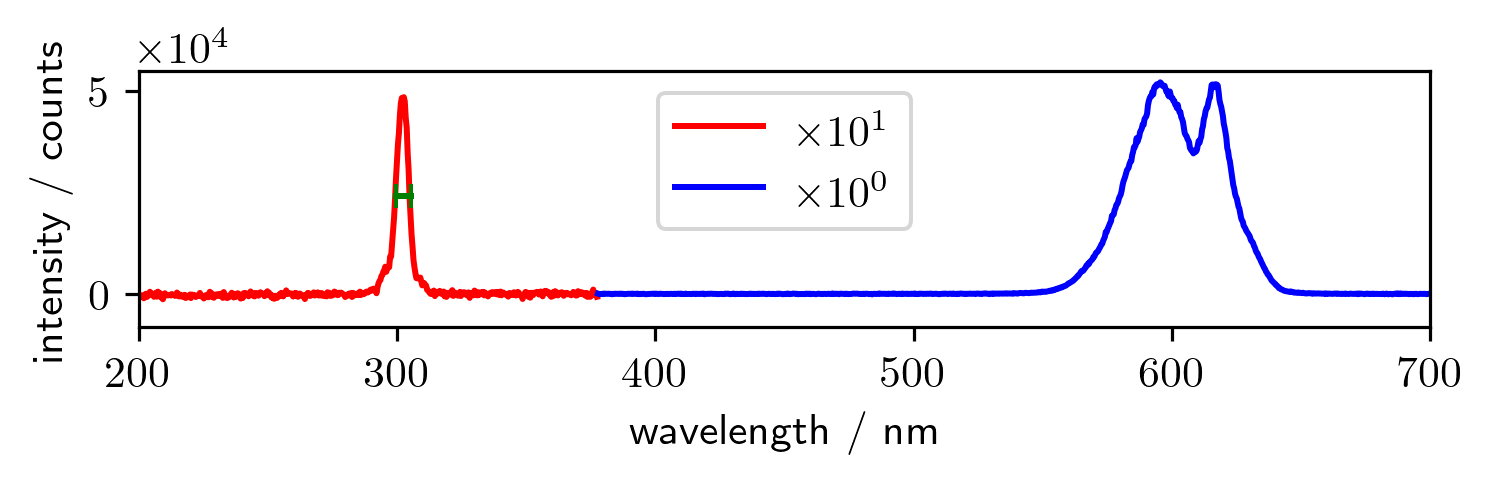
\includegraphics[scale=1]{images/spectra/SpectrumExampleNoFilter_300nm.png}
\caption[Example of \qty{300}{\nano\meter} SHG probe spectrum.]{Example of \qty{300}{\nano\meter} SHG probe spectrum.\\600 nm fundamental SHG\label{fig:specSHG300nm}\\ FWHM$_{SHG}$ = \SI{6}{\nano\meter}}
\end{figure}
%\subsubsection{Operation}
\paragraph{Setting up}
The task of setting up the SHG stage is non trivial regarding proper alignment and linear stage positioning, such that the ~5 cm of travel are sufficient to adjust for the chromatic focal shift within the targeted wavelength range for probe. This task often ends up being trial and error in correspondence to checking multiple wavelengths. The cage lenses have to be in their correct positions first.\newline
Use irises to shape the probe beam to an acceptable Gaussian shape while avoiding diffraction effects. Optimally the incoming beam is level with the table, since any inclination will introduce an astigmatism, depending on the rear lens position. Irises may also be used as a useful reference when adjusting an already working setup.\newline
Begin with the first lens in the path leaving enough space for the linear stage and the SHG crystal to the next static optic. Set lens centered regarding beam. Use the irises in front of the lens to adjust the reflection on the lens surface to return in the incoming beam path.\newline
Place the rear stage lens and once again adjust for center position. One may again use the reflection and additionally the transmitted beam to tell if the stage is parallel to the beam path. The center of the beam should not move when translating the stage and the expansion of the beam diameter should be as radial-symmetric as possible. Adjusting via the reflection is not such a clear indication of alignment here, as there are multiple convex surfaces in play at this point, leading to multiple reflected beams, that may not be in full accordance with each other. For this it usually was chosen to put the highest intensity reflected spot, which refers to the final glass/air surface of the second lens, into the incoming beam path. This spot is also focused, which makes adjustment easier.\newline
Finally one can adjust mirrors after the stage to get an image on the camera again, as even relatively minute changes in alignment will lead to some beam offset and change in direction. Translating the stage then will give an indication of how well the SHG stage is set up regarding astigmatism, which can be seen as non symmetric expansion of the beam. However beware that the mirror outcoupling in the cage also influences the way a change in focus is experienced, due to deviations from an orthogonal inclination angle to the sensor.




\paragraph{For measurements}
To find SHG intensity approach the focal spot from the incoming beam direction and adjust SHG crystal until sufficient output power is achieved. It proved better to start with higher irradiance and only use more ND filters later. The output second harmonic beam tends to have better beam shapes if the crystal is right in focus and the power is only regulated by ND filters, instead of reducing irradiance by translating the crystal out of focus. It may be beneficial to write down crystal orientations for difficult to find wavelength settings.\newline
Adjust the linear stage such that there is no lateral movement. The current linear stage slide is mounted in a way that can rotate a bit, if force is applied at the corners. It may be necessary to do this and have the stage "snap back" to make sure it will not move during the measurement. This can be checked after the measurement by checking the overlap again.\\
Schott glass filters may be used to reduce the intensity of the fundamental wavelength. In some cases interferometric mirrors may be needed to remove background from the NOPA; however they may not be used to filter the fundamental of the second harmonic since they are opaque in the UV range. The increased temporal pulse-length is acceptable due to the long lived nature of the excited states of the sample used. Internal transmittance spectra of the filters used, which in some cases may be combined, are shown in fig. \ref{fig:SchottFilters}.

\begin{figure}[hbtp]
\centering
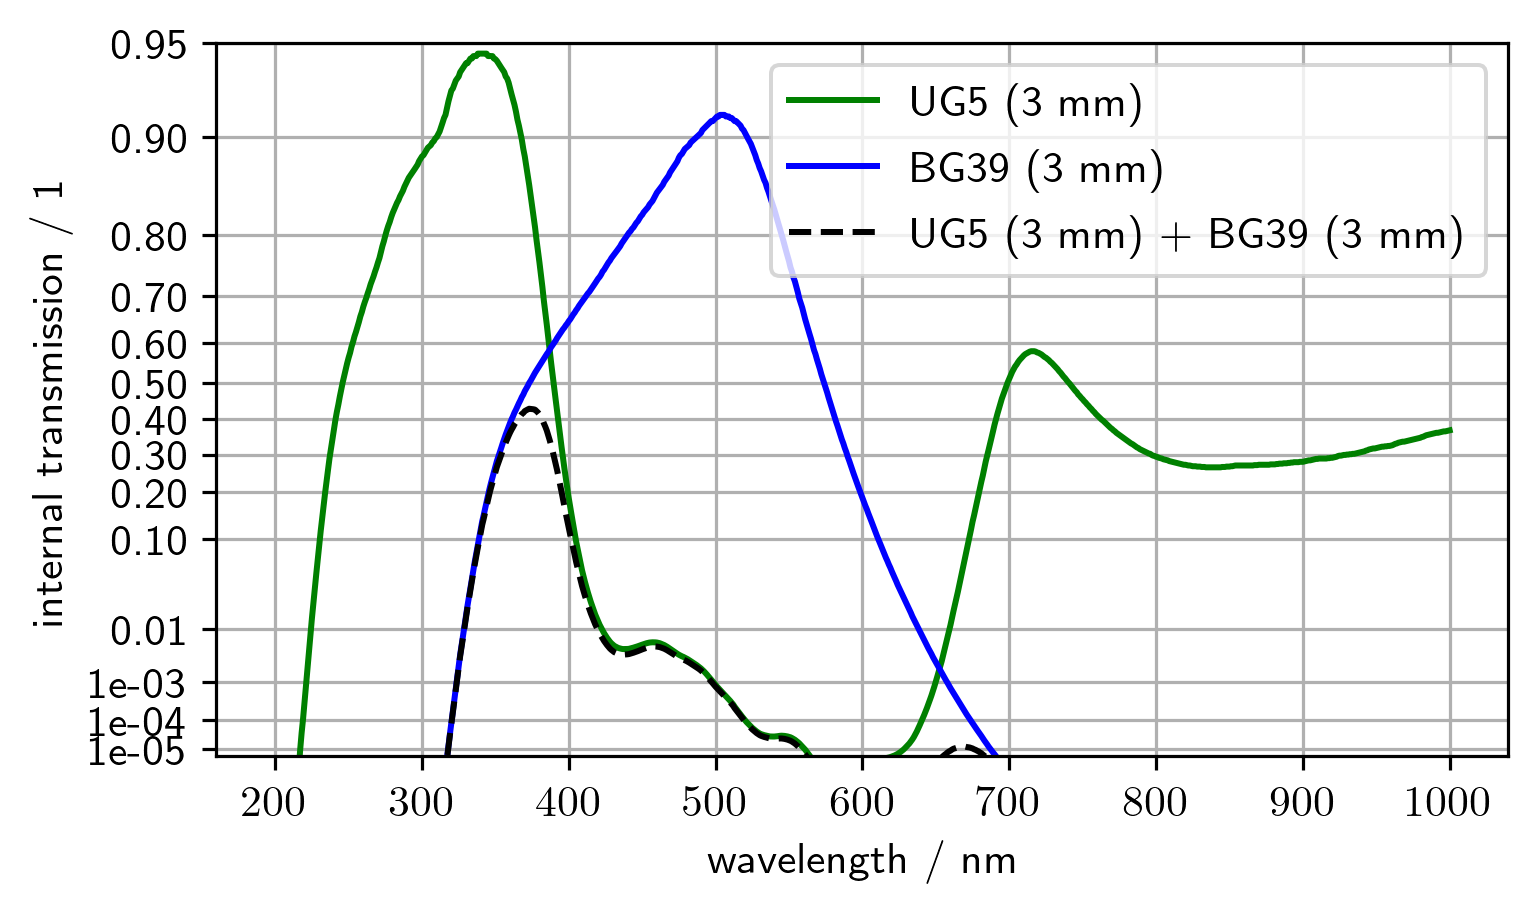
\includegraphics[scale = 1]{images/SchottFiltersFromTool.png}
\caption[Internal transmittance of Schott glass filters in 3 mm used for fundamental filtering.]{Internal transmittance of Schott glass filters in 3 mm used for fundamental filtering.\label{fig:SchottFilters} Data taken from the SCHOTT filter calculation tool.\protect{\cite{SCHOTT2023}}}
\end{figure}

A polariser may be used alternatively to glass filters. Reasoning is that for the BBO only type 1 phase-matching is possible with a singular fundamental polarized beam, where the fundamental polarization (ordinary polarization) is orthogonal to the SHG output (extraordinary polarization). Note however that the wire grid type polariser has a falling external transmission and falling extinction ratio for short wavelengths in the UV. Thus mainly the fundamental intensity is modulated with rotation of the polariser.

\subsection{Detector setup}
The detectors themselves are the same as described in Schwarzl et al\cite{Schwarzl2022}. Matlab software for the measurements was devised by Pascal Heim. For the measurements \text{detector A} was used at all times in combination with a picoscope 5442D. An isosceles, UV translucent, prism is inserted after the cage, to remove any remainders of the fundamental probe wavelength at the detector. To improve this separation an extra iris may be used immediately in front of the detector.\\
The prism should be placed such that the angle between pump and probe is further increased, as this can help reach full pump rejection without any other filters or beamblocks involved. The prism is important as the fundamental light for SHG tends to be on the extended absorption feature for SQIB, which has a far higher transient response than the second harmonic wavelengths. The prism is used since the detector is so sensitive, that further filters would not guarantee sufficient fundamental rejection. For each change of the probe the mirror coupling into the prism should be adjusted for maximum intensity of the probe on the detector, which can be monitored using the \text{fourierDetector()} matlab program.\\
The detector has a maximum peak to peak voltage (Vpp) of approximately \qty	{3}{\volt}, before the response no longer is linear. Vpp should for that reason be kept below \qty{3}{\volt} to avoid response problems and thus systematic errors in the measurement.
\subsection{Adjusting overlap without achromatic optics}\label{sec:overlapChromaticAberration}
This section introduces the solution to working with non-achromatic optics in this transient absorption microscopy setup. Some of the attempted, but inevitably abandoned, ideas and tests are introduced after going through the final solution of a camera in the mirror plane of the sample surface.
\paragraph{General overlap adjustment}
Pump-probe overlap adjustments are done using a camera, onto which the sample plane is imaged. This is combined with a fitting program, which fits a Gaussian point spread function to the beam image. From this a center position as well as the FWHM of the point spread function can be determined and used to move the point spread functions on top of each other. An explanation on how to use the software is in sec. \ref{sec:LiveFitting}.

\paragraph{The problem of achromatic optics}
One of the main issues that had to be addressed was the change from achromatic objectives to uncoated plano-convex lenses within the cage.
This is emphasized especially by plotting the wavelength dependence of the focal length, see fig. \ref{fig:ChromFocalShift}, as defined by the lensmaker equation for the lenses used:
\begin{equation}
\frac{1}{f} = (n-1) \left[\frac{1}{R_1} - \frac{1}{R_2} + \frac{(n-1)d}{n R_1 R_2}\right]
\end{equation}
\begin{figure}[h]
\centering
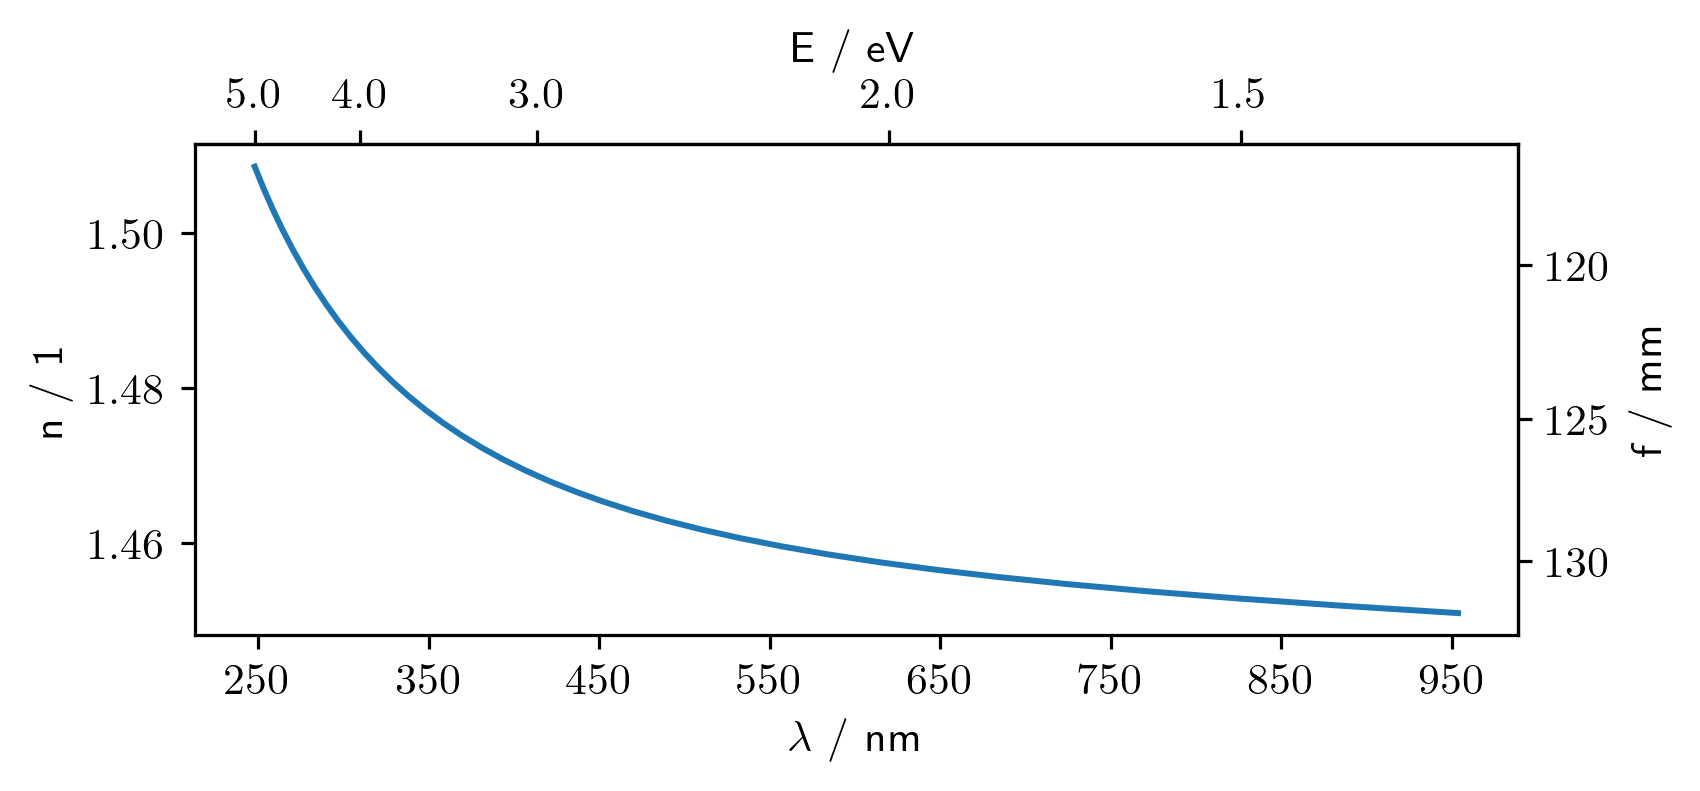
\includegraphics[scale = 1]{images/ChromaticFocalShiftandDispersionUVFS.png} 
\caption{Refractive index change and focal shift for UV fused silica plano-convex lenses used in cage setup.\protect{\cite{Malitson:65}}\label{fig:ChromFocalShift}}
\end{figure}

Furthermore the depth of focus may be visualized by plotting the beam waist diameter over distance from the focal point for several relevant focal lengths in fig. \ref{fig:beamWaistCompendium}. The beam waist is calculated by the formula for focusing a Gaussian beam at any position in relation to focal length. The change of the depth of focus (DOF) and thus the change in beam waist diameter for a specific distance from the focal point of the corresponding wavelength decreases for higher photon energies. An assumption has to be made for the waist distance $s^\shortmid$ from the lens. When $s^\shortmid$ is close to the focal length the minimum beam waist is located at the focal length. Stronger deviations are still tolerable as long as $s^\shortmid \ll z_\text{rayleigh}$, as both the minimum beam waist is still close to the focal length and the intensity behaviour is still close to what is shown in fig. \ref{fig:beamWaistDOF}. For $s^\shortmid \approx z_\text{rayleigh}$ the wavefront distortion leads to much smaller focus with a fast falloff and noticeable a shift of the minimal beam waist. $s^\shortmid \gg z_\text{rayleigh}$ the wavefront is nearly planar again, but the focus is smaller and falls off faster still. Note that $s^\shortmid$ cannot be greater than the rayleigh range, as this formula expects the beam diameter for $s^\shortmid \gg z_\text{rayleigh}$ to get very large according to the beam diameter immediately ahead of the lens $w_l = w_0 [1+\left(\frac{s^\shortmid}{z_\text{rayleigh}}\right)^2]^\frac{1}{2}$, which is not the case here. So it is assumed that $w_l \approx w_0$ and thus $s^\shortmid \ll z_\text{rayleigh}$, making the plot assumptions valid.\cite{Li1994}

\begin{figure}[htbp]
\centering
\begin{subfigure}[t]{0.49\textwidth}
\centering
\includegraphics[scale=1]{images/BeamWaist_Wavs_2.5mm.png} 
\subcaption{Beam waist for wavelengths at \mbox{2.5 mm} input beam diameter.}
\end{subfigure}
\hfill
\begin{subfigure}[t]{0.49\textwidth}
\centering
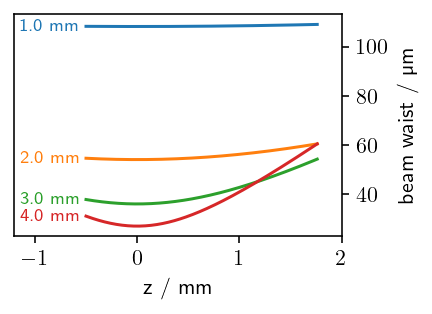
\includegraphics[scale=1]{images/BeamWaist_inputWidth_653nm.png} 
\subcaption{Beam waist for several input beam diameters at 653 nm.}
\end{subfigure}
\hfill
\\
\centering
\begin{subfigure}[t]{\textwidth}
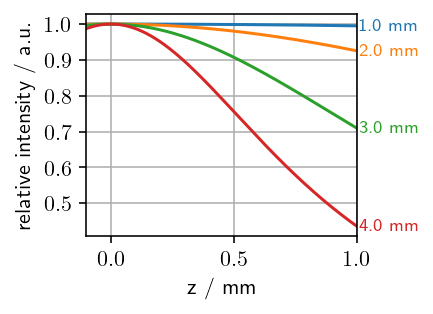
\includegraphics[scale=1]{images/DOFintensity_inputWidth_653nm.png} 
\subcaption{Maximum intensity relative to maximum intensity in focus depending on input beam width at 653 nm. \label{fig:beamWaistDOF}}
\end{subfigure}
\caption[Changes of simulated Gaussian beam profile width and intensity for lenses used in the cage system.]{Changes of simulated Gaussian beam profile width and intensity for lenses used in the cage system, EKSMA 110-1216ET with 125 mm focal length at 355 nm, with z being the distance of the assumed imaging plane from the focal plane.  Assuming perfect Gaussian input beam. Beam waist calculated as per Li and Katz\cite{Li1994}. Input beam waist distance set to focal length. \label{fig:beamWaistCompendium}}
\end{figure}

%This issue is of fundamental nature and a few attempts were made until the following solution was found:

\paragraph{Sample mirror path}\label{SampleMirrorCamera}
The option that finally won out is decoupling the beams after the frontal cage lens and imaging onto a camera that is in the mirror plane of the sample surface. This method requires a process for consistent placement of the mirror within the cage and a way to move the camera into the mirror plane of the sample.\\


\paragraph{Setup}
To achieve a reproducible mirror placement a 45 degree mirror insert for the cage is used, which was designed to rest on top of the cage system rails. This drop in mirror mount was 3d printed for adjustability and has proven to be consistent enough to allow for this method to work. The result of a brief test of placement reproducibility may be seen in fig. \ref{fig:DropinStudy}. \\
An advantage of PLA, as opposed to an aluminium block with the negative of the rails cut into it, is that its mechanical compliance allows proper sliding into place, whereas aluminium "gripped" onto the rails making it hard to get consistent placement. This may be improved by cutting the rail negative in aluminium even larger. However this still presents one with the problem of how to mount the mirror to the mount. Super-glueing  the mirror to a aluminium mount was attempted for a quick trial, but this proved to not be a long lived connection.\\
\begin{figure}[hbtp]
\centering
\begin{subfigure}[t]{0.66\textwidth}
\begin{subfigure}[t]{0.45\columnwidth}
\centering
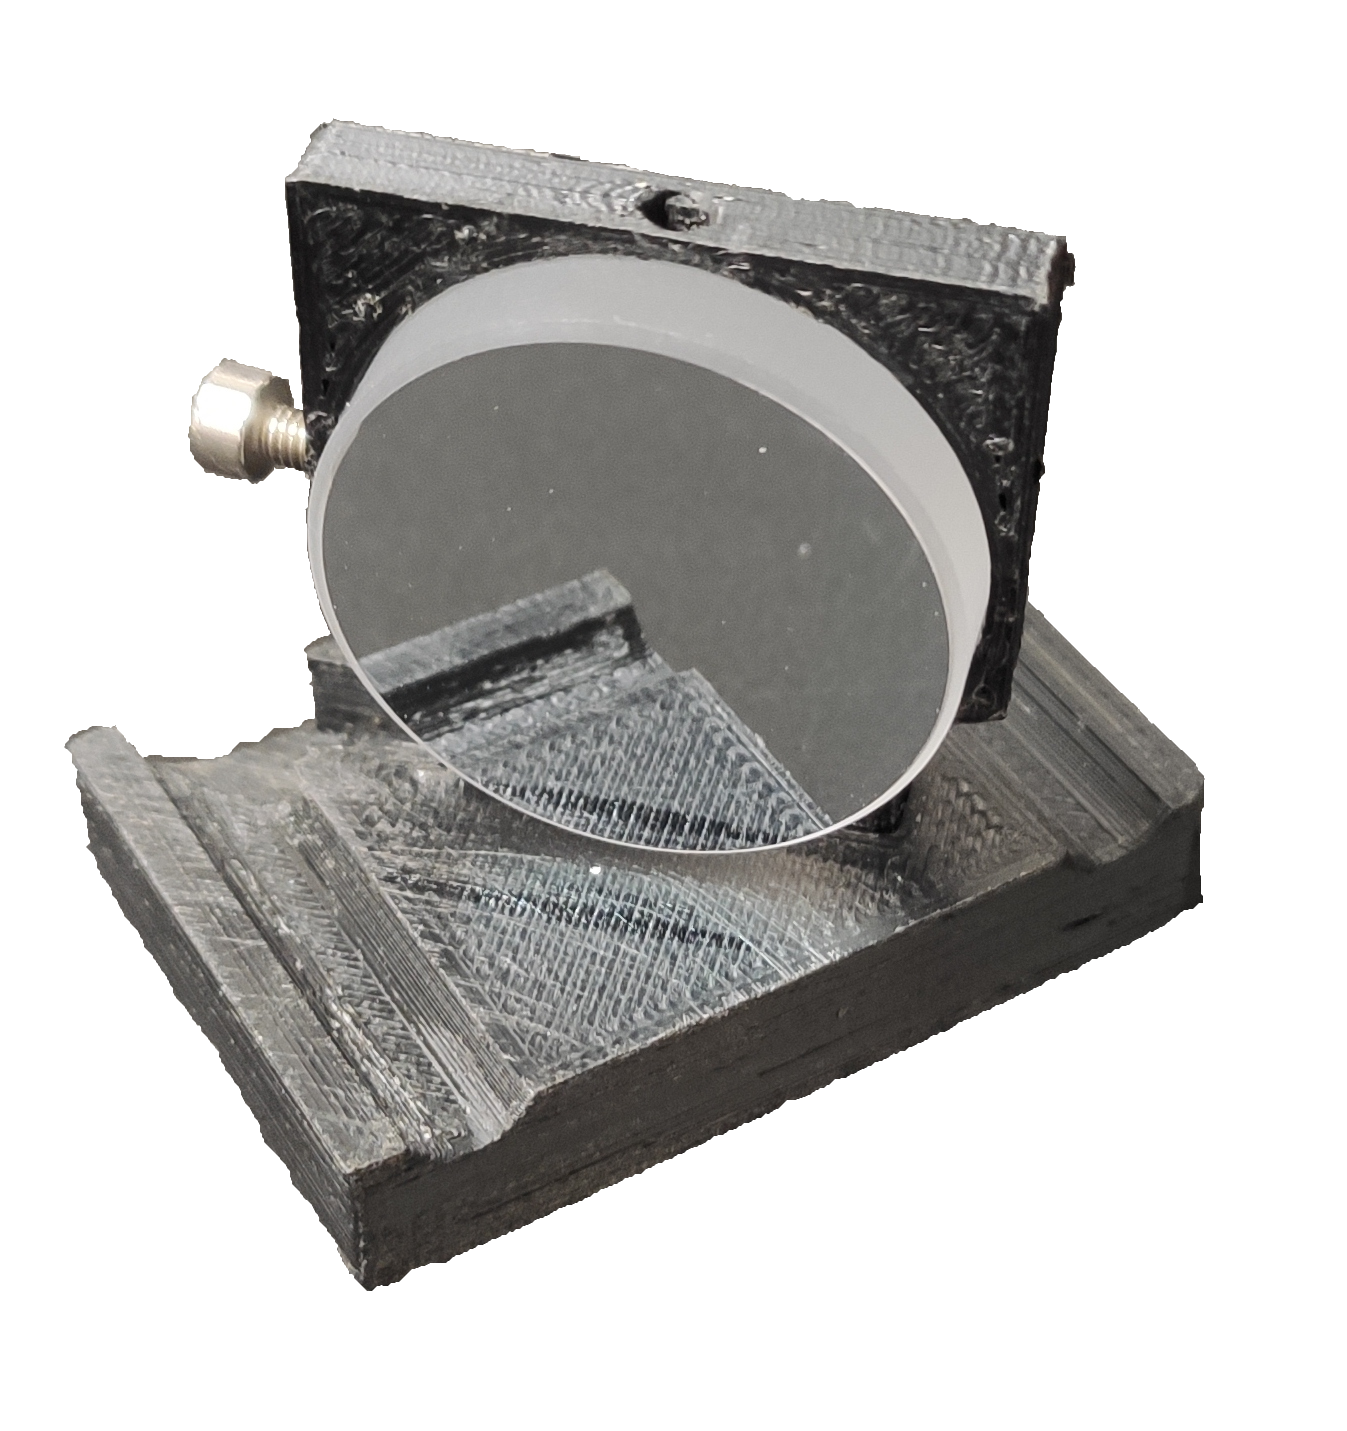
\includegraphics[width=\columnwidth]{images/TAM/MirrorDropInFrontFree.png}
\end{subfigure}
\hfill
\centering
\begin{subfigure}[t]{0.45\columnwidth}
\centering
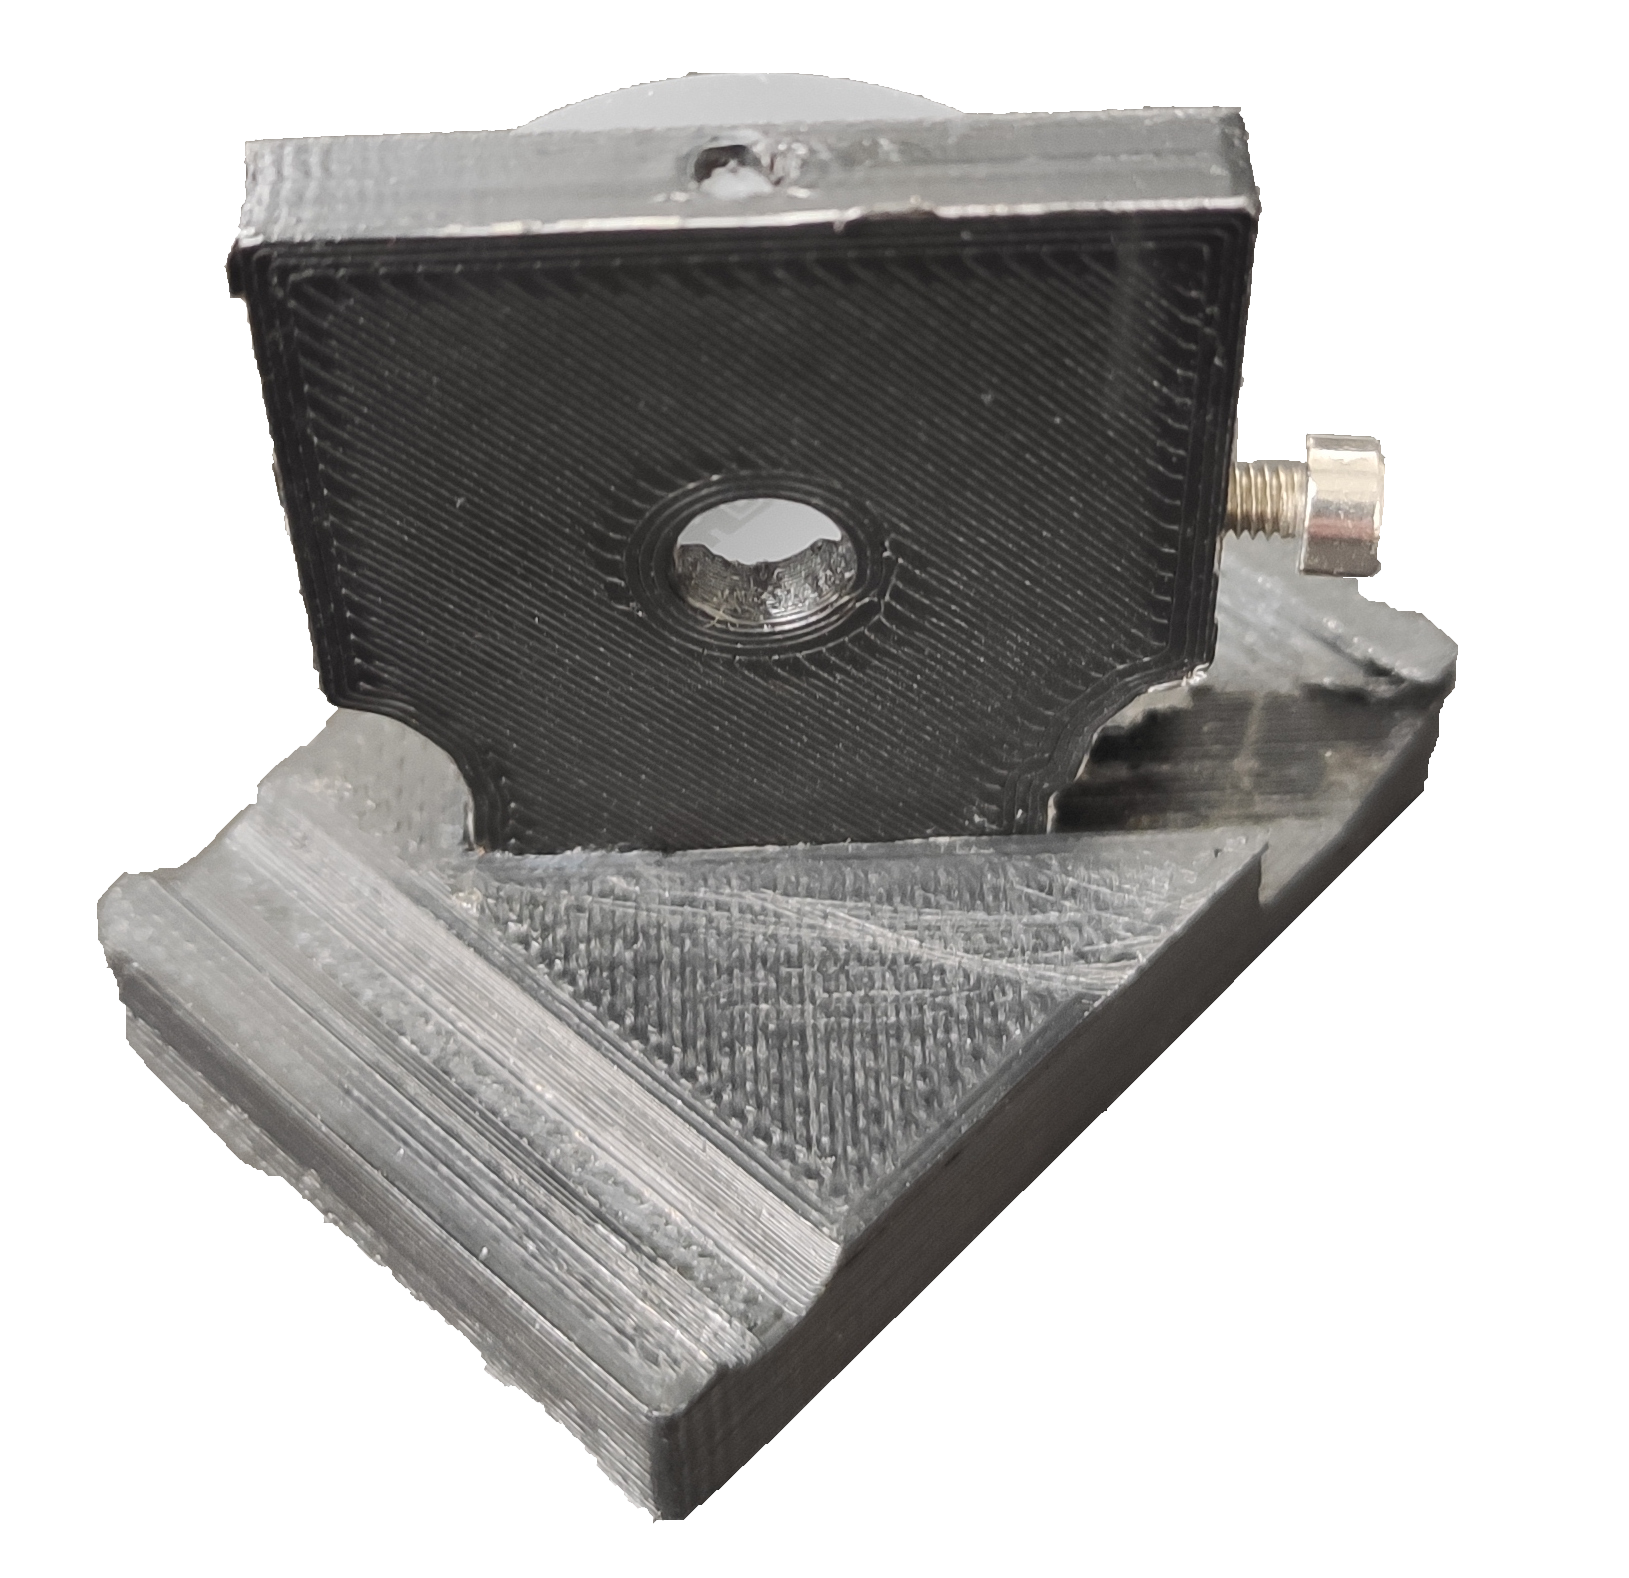
\includegraphics[width=\columnwidth]{images/TAM/MirrorDropInBackFree.png}
\end{subfigure}
\caption{3d printed drop-in mount with UV enhanced Al mirror.
The mount is designed for use with 30 mm cage systems like the Thorlabs system and may be parametrically adjusted.
It is printed in two parts, which use joinery to interlink and are fixed together with super-glue to avoid movement.
The mirror may be attached via a friction fit and a flat-head screw.\label{fig:drop-in-Mirror-mount}}
\end{subfigure}
\hfill
\centering
\begin{subfigure}[t]{0.3\textwidth}
\centering
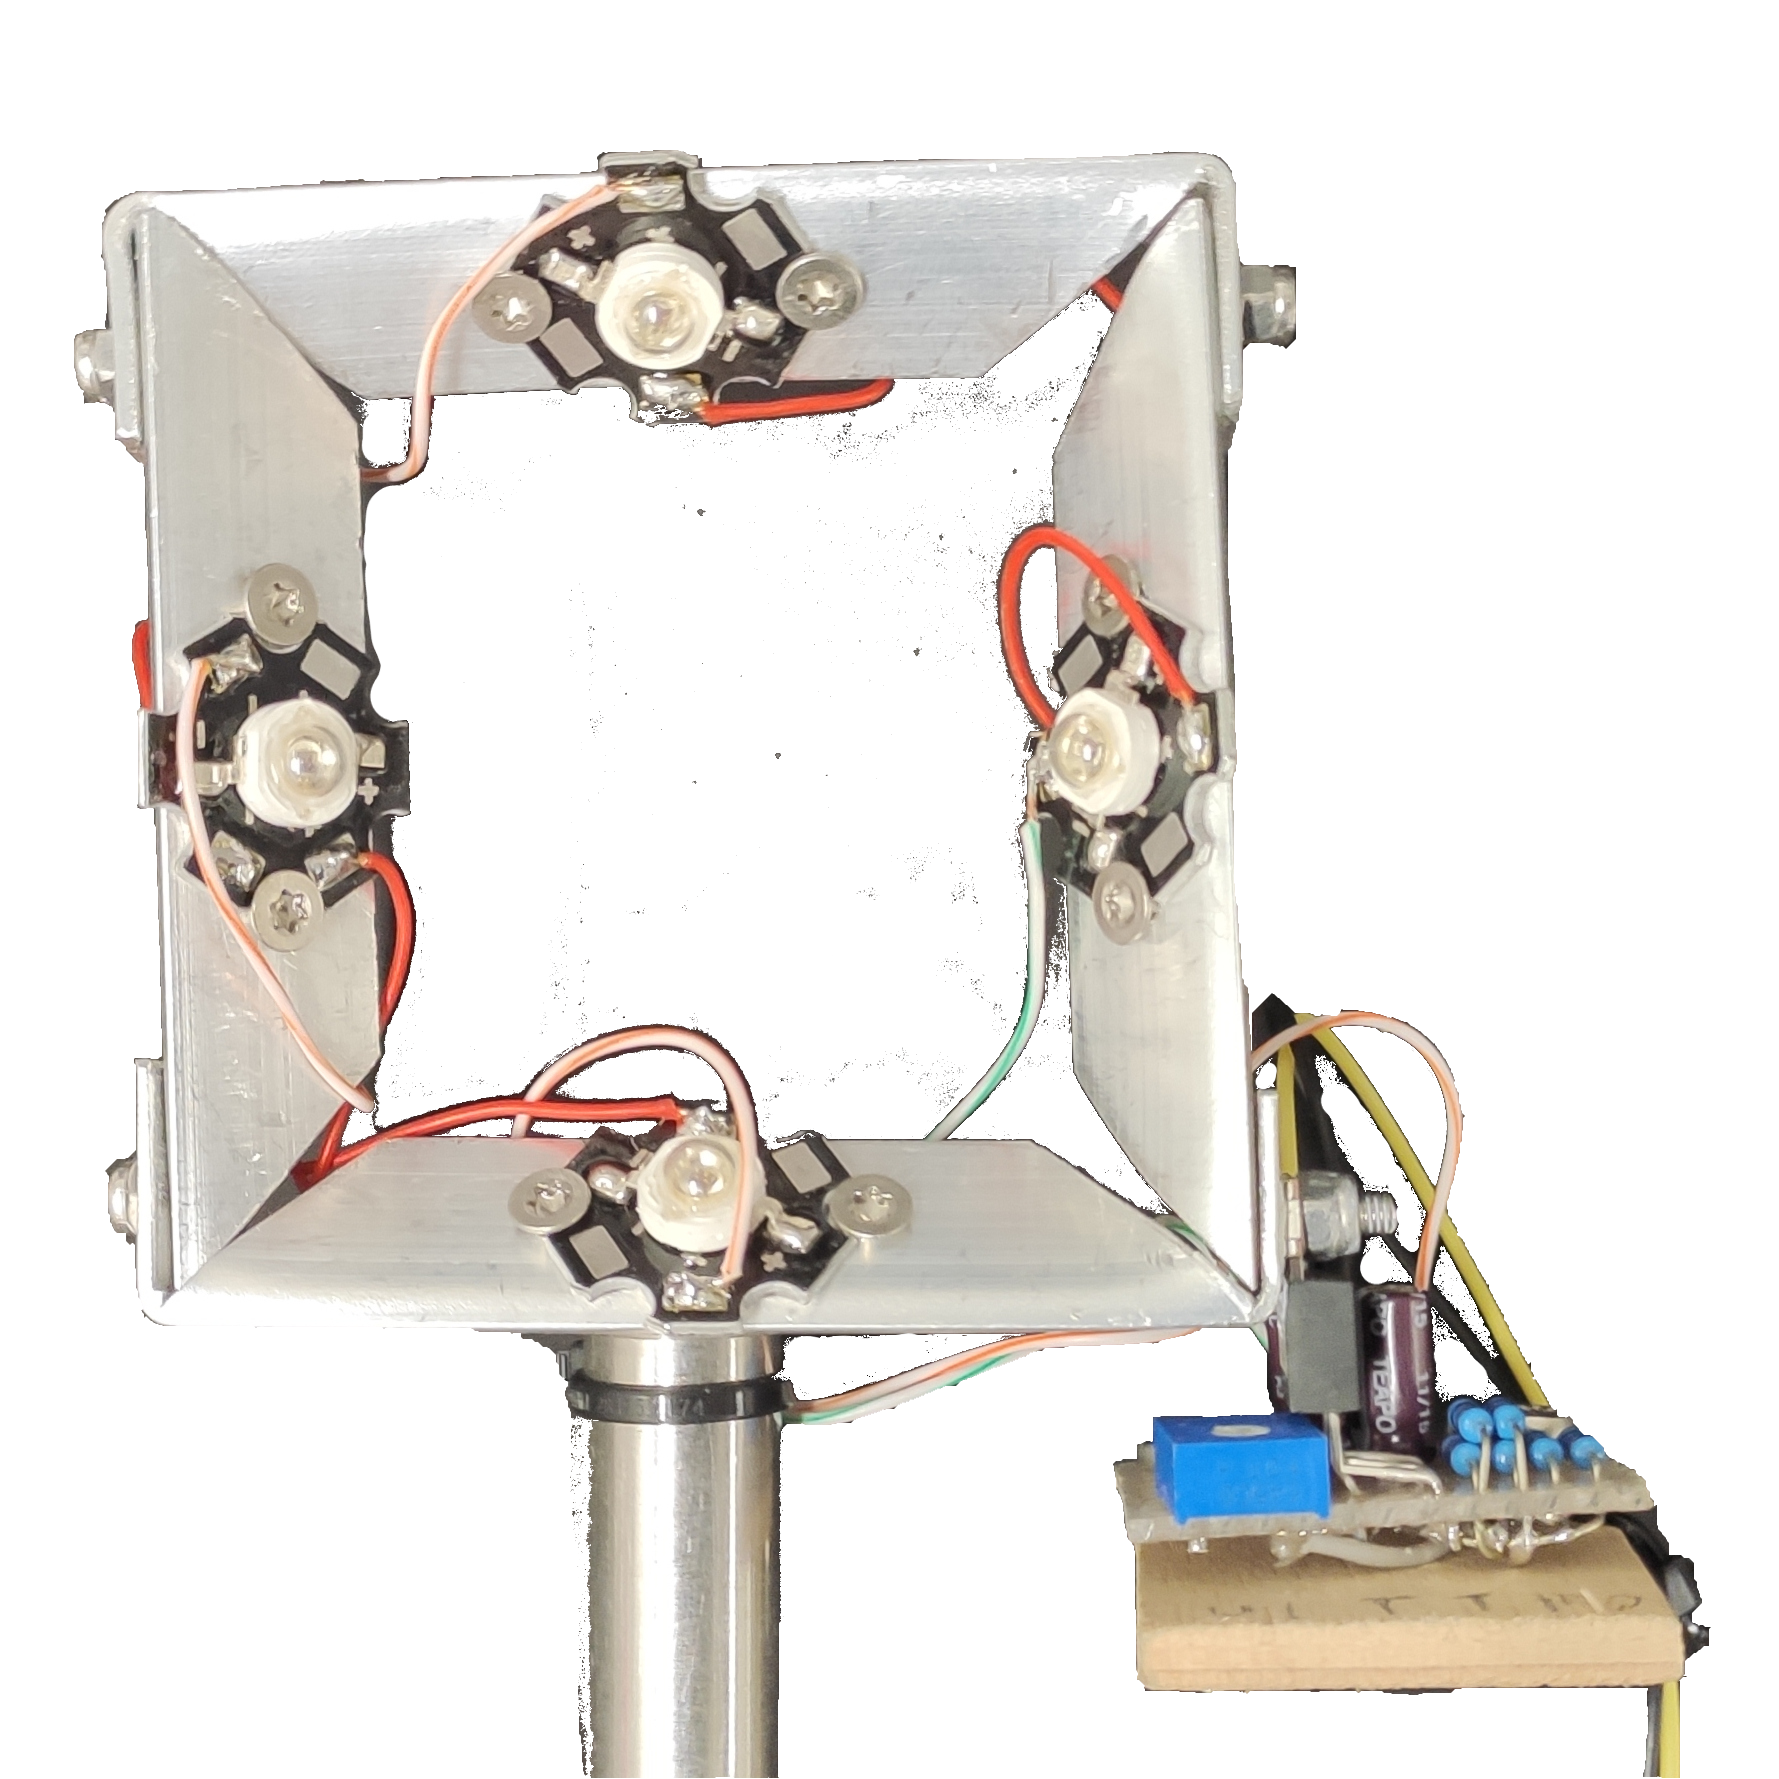
\includegraphics[width=\columnwidth]{images/TAM/RingLightFrontFree.png}
\caption{Ring light with red LEDs adjacent to pump wavelength. Spectrum may be seen in fig. \ref{fig:calibLEDspectrum}.\label{fig:ringLight}}
\end{subfigure}
\caption{Auxilary tools for alignment, focusing and use of SHG extension setup.}
\end{figure}


The 3d printed mount can be seen in fig. \ref{fig:drop-in-Mirror-mount}.
Considerations regarding use of rubber bands or 3d printed fittings were made; however, it turns out just by moving the mirror drop-in mount against a solid surface, such as one of the cage plates holding the rails, the beam position is sufficiently reproducible for the sensor resolution of the camera used. Some care should be taken to adjust the tilt angle regarding the vertical projection axis, however the influence of that should be minimal considering both pump and probe are always calibrated at the same mirror setting. Additionally the beam waist diameter should not change by a drastic amount considering the theoretical variation seen in fig. \ref{fig:beamWaistCompendium}.\\

The lighting for imaging the rear sample onto the camera via the rear lens is done using a ring light with 4 LEDs, which have a spectral intensity distribution close to the intended pump beam. The spectrum can be seen in fig. \ref{fig:calibLEDspectrum}.
It has proven beneficial to illuminate so that only scattered light is detected, as this improves contrast akin to reflected darkfield microscopy.\cite{Zeiss} Thus the LED ring is placed behind the sample, on the side of the rear camera. As this means reduced total intensity, any light not scattered by the sample or reflected from nearby surfaces needs to be blocked. For this purpose carton is placed around the rear cage rails, blocking any light reflected by the sample mount from reaching the camera.
%The LEDs are mounted onto a square aluminium frame and are angled towards the sample to illuminate it evenly. To properly setup the focus light that not passing through the lens has to be minimized or contrast will be lost. To focus properly a small scratch is introduced to the edge of the sample, which allows better contrast for focusing as well and allows to focus closer to the center to the layer than to the top or bottom of the layer. (eh questionable, think better)

\paragraph{Calibration method}
The rear lens is set to image the sample plane onto the rear camera as described in sec. \ref{sec:cageSetup}. A pump adjacent wavelength is used to illuminate the sample from the detector side. This is done to be able to use the pump beam as a reference for the cage system, as the front focus for the sample and the rear focus for the rear camera are both calibrated using a wavelength with very little chromatic focal shift from the pump wavelength. A two step process is then used to set the position of the front camera, in the mirrored sample path, correctly:
\begin{figure}[hbtp]
\centering
\begin{subfigure}[b]{0.5\linewidth}
\centering
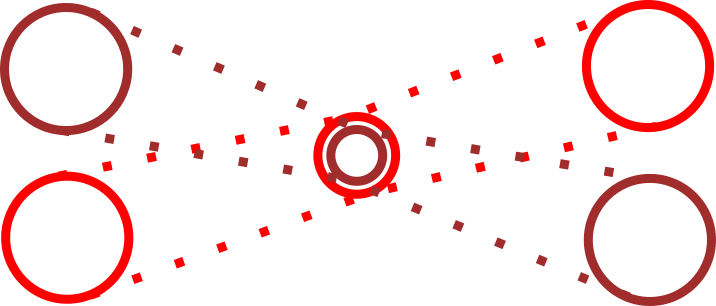
\includegraphics[scale=1]{images/ArtrayCalibrationIllustration_Good.png}
\caption{Good calibration with beams crossing in pump focus.}
\end{subfigure}\hfill
\begin{subfigure}[b]{0.5\linewidth}
\centering
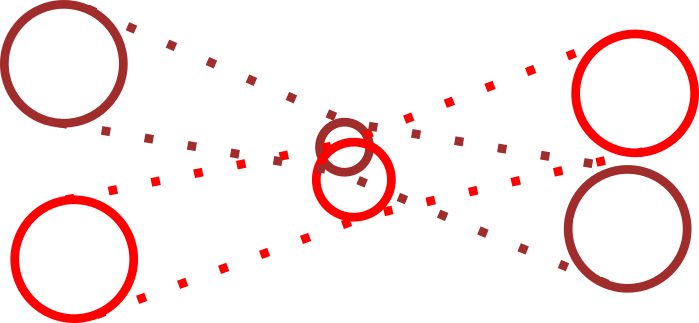
\includegraphics[scale=1]{images/ArtrayCalibrationIllustration_Bad.png}
\caption{Bad calibration with beams not crossing in pump focus.}
\end{subfigure}
\caption[Illustration of front camera position calibration.]{Illustration of front camera position calibration. Shows progression of beam sizes when moving frontal camera closer or farther away from the cage. Note that the probe beam does not necessarily have to be minimal when pump and probe overlap, however pump diameter needs to be minimal.\label{fig:calibrationArtrayIllustration}}
\end{figure}

\begin{enumerate}
\item It may seem like a good idea to just minimize the beam waist of the imaged pump beam. However due to effects of the image inversion on fitting, this does not work well. Inversion being the outer features of the beam profile passing through the center. Adjust the frontal camera distance so, that the pump beam profile is right before inversion, due to passing through the focal point. The intensity, given by fitting, still rises a tiny bit beyond that point. Attention has to be paid to not go into inversion, which is hard to tell by eye. Example images for pump \qty{653}{\nano\meter} calibration of the frontal Artray camera are shown in fig. \ref{fig:pumpCalibComparison}. After a first good calibration this could be done by comparing the fitted intensity value/FWHM of the beam profile, as long as the pump beam path did not change. Placement of ND filters in front of the camera or in front of the cage does matter, as swapping the position changes the beam profile. This is due to a change in optical path length, when a filter is inserted after the lens. Reason is the refractive index of the ND filter differing from the refractive index of air.
\item Set the probe to the same or an adjacent wavelength to the pump and set overlap using the rear camera. Due to beam paths and possible aberrations this may be a tedious process and not completely accurate. Check the overlap on the frontal camera by moving the camera back and forth while observing if the beams cross through their centers, as illustrated in fig. \ref{fig:calibrationArtrayIllustration}. If that is the case the pump probe overlap should be optimal and the frontal camera can be set to the optimum position of this overlap. Take reference TA measurements if possible to check if there is an improvement from the purely rear camera based position.
\end{enumerate}
\begin{figure}[hbtp]
\centering
\begin{subfigure}[b]{0.32\linewidth}
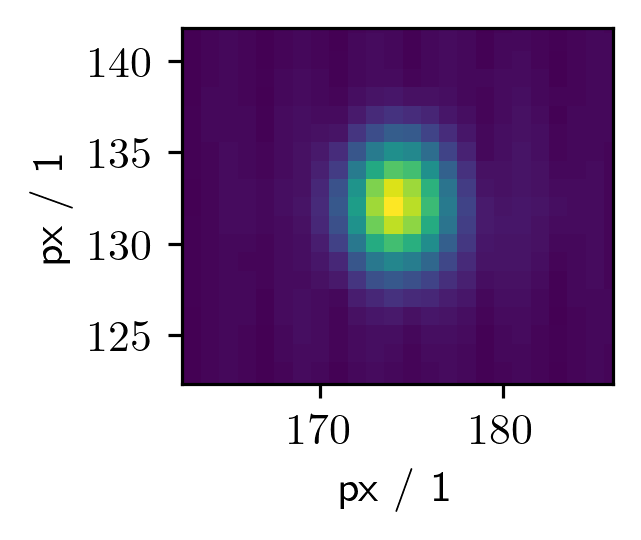
\includegraphics[scale=1]{images/CalibComparison/fullOptimizedComparisonCalib.png} 
\caption{Optimal calibration}
\end{subfigure}\hfill
\begin{subfigure}[b]{0.32\linewidth}
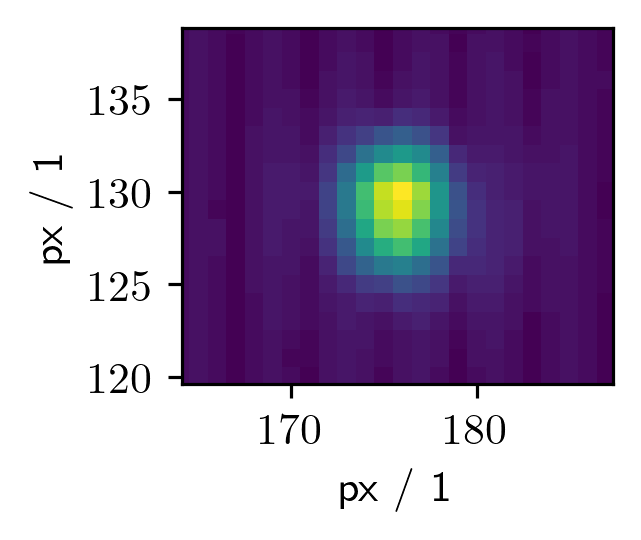
\includegraphics[scale=1]{images/CalibComparison/betterComparisonCalib.png} 
\caption{Plain calibration}
\end{subfigure}\hfill
\begin{subfigure}[b]{0.32\linewidth}
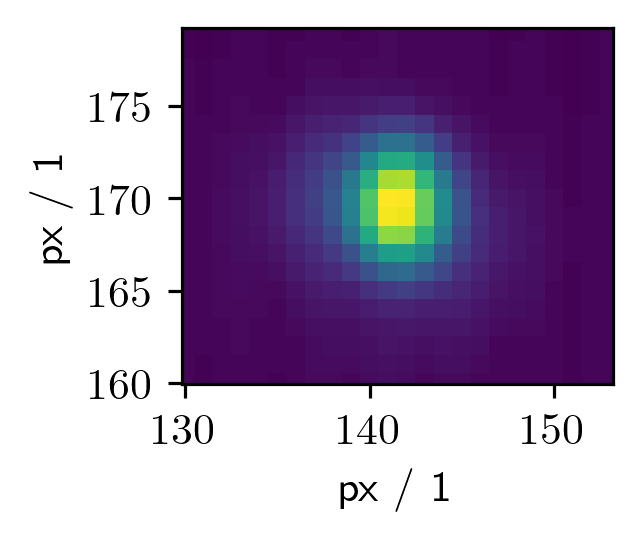
\includegraphics[scale=1]{images/CalibComparison/worstComparisonCalib.png}
\caption{Calibration in inversion}
\end{subfigure}
\caption[Comparison of different frontal camera position settings for calibration process.]{Comparison of different frontal camera position settings for pump \qty{653}{\nano\meter}. In b.) the positioning is based on beam shape and frontal camera overlap, while in a.) additionally the rear camera overlap is considered and adjustment is checked with a transient absorption measurement. Overlap and transient absorption measurements here use a probe of \qty{680}{\nano\meter}. c.) is based only on beam shape of the frontal camera and is too far into inversion of the beam. Colour ranges are normalised individually.\label{fig:pumpCalibComparison}}
\end{figure}

The conversion factor $\frac{\si{\micro\meter}}{\text{px}}$ is taken from a comparison of the fit values of the reference rear camera pump point spread function to the front camera, see below in "Regular focusing after cage". When imaging the pump beam through the sample, attention has to be paid to any sample irregularities which may change the point spread function, which is why an averaging over multiple sample spots\footnote{Matlab function FrontFocusAverage} is applied. Attention has to be paid to possible aberrations on the rear camera due to the pump path usually being off center. For example when the pump path passes close to the bottom of the lens only the x axis fit of the beam shape is used to compare the beam sizes. For the same reason it may not be a good idea to set the front camera position by comparing aspect ratios to the rear camera, as this has not shown as a reliable way to get good measurements. However when imaging the sample with the ring-light variation or spherical aberration over the image is minimal. The light for imaging is not as directed as the pump, meaning the effect may be less than for a slightly angled pump beam. 

Comparing the beam point spread function of the pump on the rear and front camera, the front camera does not return the expected physical pixel (\qty{5.6}{\micro\meter}) dimensions as the calculated $\approx\mathrm{6.9\frac{\mu m}{pixel}}$ ratio. If this is a miscalibration, then it would break the comparability of measurements not made with the same calibration setting, as this influences calculated irradiances. However within a measurement series at the same calibration there is no relative change or influence and measurements are directly comparable. Reason for this mismatch is unknown, however considering the lack of pixel density, with no more than 7 pixels over the FWHM, this may be a limit of the camera. If the calibration is correct then this implies a better focus, meaning a smaller focus spot, on the frontal camera than the rear camera.
%\textit{The pixel scale factor being larger than the pixel size means that the focus size is smaller on the front camera than on the rear camera. For one this may be an influence of aberrations and other imaging errors. Otherwise this would mean that this is not so comparable and that the absolute corrected output values of the thesis may not be directly compared between different calibration settings, as the peak irradiance would be calculated incorrectly. Anything I can do with that? On the other hand the pixel density just isn't high enough to make a good description.}

\paragraph{Use}
After calibration no changes, other than changing ND filters or polarisation with a $\lambda/2$ waveplate, to the pump beam path are to be made. The calibration is only valid for the set pump position. During use care has to be taken that there is no clipping at the drop in mirror, as this would obviously ruin the perceived beam shape. As mentioned before, if there is an ND filter directly in front of the camera for fitting of one beam, then there should be an ND filter there as well for the other beam, as this may cause a change in the observed beam shape. For high energy SHG light absorptive ND filters have far stronger absorption than for their calibrated range, thus they may need to be swapped for a lower value. With this effect an observed "amplification" of fundamental light from the SHG stage is introduced, which is further increased by the CMOS sensor having lower quantum efficiency at these wavelengths. Thus it is important to check if the fundamental wavelength has a strong influence on the observed point spread function.\\
This can be done by introducing more glass filters, in case their absorption of the fundamental is lacking for the wavelength. The glass filters may be removed afterwards if the detector is using the prism setup, which removes the fundamental wavelength from the measurement.\\
Another option to check is to remove the fundamental filter completely and check the position of the fundamental focus spot in relation to the SHG focus spot, which will be different due to chromatic focal shift.

\paragraph{Regular focusing after cage}\label{regRearFocus}
This is the option used for the regular TAM setup as described in section \ref{RegTAM}. The last mirror in front of the detector is simply removed to reveal a camera behind it. The rear cage objective is focused onto the rear camera using white light from an LED torch or similar light sources in transmission. A calibration of sensor pixels to physical dimensions, after focusing, is done by moving the sample stage by an arbitrary distance and calculating the pixel shift from the sample image, see example image in fig. \ref{fig:micrometerToPxExample}. Afterwards the front objective is moved such that a satisfactory point spread function of the beam is seen on the rear camera. For the SHG setup this pump point spread function needs to be minimal in size.

This is sufficient as the achromatic objectives ensure a very similar focus for all wavelengths between 400 nm and 940 nm. The rear objective is focused to image the plane of the sample onto the rear camera. Thus in use it simply projects the point spread function of the beams in the plane of the sample onto the camera. Moving the front objective adjusts the part of the focusing beam cone, and thus the size of the slice of the beam, which interacts with the sample. This works for both pump and probe. Since the focal length of the lenses varies wildly in the UV this is not an option for the UV extension.
\paragraph{Conversion screen for overlap adjustment}
An idea, later on abandoned for impracticality, was to use a screen as a placeholder for the sample to then be imaged onto the rear camera using the rear cage lens. This method has several requirements:
\begin{itemize}
\item The screen needs to allow for diffuse imaging of the sample without disturbing the beam shape too much.
\item A method of placing the screen in the sample plane with very little deviation.
\item Any UV or near UV light needs to be converted to the visible region, where the focal length difference becomes negligible.
\end{itemize}

The requirement for diffuse imaging is simple. Any incident collimation or focusing action of the beam needs to be lost to actually image the sample plane, where the screen is placed at. The requirement is less stringent for wavelengths close to a chosen wavelength, to which the setup would be calibrated to, as the lenses would image the beam fine for that wavelength.\\

Placement of the screen in the sample plane may be done with 3d printed sample mounts with variable spacers, which would have to be adjusted for every different kinds of sample substrates. Sample layer thickness usually is very thin, so placing the screen in the plane of the frontal substrate edge should suffice. Using a non stiff screen, such as PTFE tape, requires a slightly more sophisticated mount to avoid deformation and thus variation in screen distance from the sample distance to the frontal lens. 

For the issue of UV conversion a few attempts with different dyes and paper were made, which showed varying success as to their luminescence. Generally orange gel marker (Stabilo No. 70/40), combined with paper or a transmitting substrate, seemed to work best for conversion of UV to visible light.
Standard density and lens paper did not work particularly well for conversion, unless combined with a text marker. To improve transmittance the paper was soaked with candle wax, which is naturally UV fluorescent. The fluorescence of the wax on paper alone, without the marker, was insufficient. The marker has to be applied on the opposite side of the paper ahead of soaking with wax. 

Alternative to paper, using a glass microscope slide with gelled, specifically at room temperature evaporated, Stabilo marker (No. 70/40) turned out to have decent conversion efficiency, while lacking any diffusivity.  This may be an option when adjusting the cage setup to correctly image the pump wavelength, like it is now done with the mirror camera setup. However at that time the rear focus was still set with white light instead of \qty{653}{\nano\meter} pump adjacent light, which would not have allowed for this method. Long enough wavelengths simply transmit through the glass slide and would need to be filtered, while relying on conversion of those wavelengths by the screen at reasonable intensities. An attempt at texturing the slide surface was not made, due to unavailability of suitable processing methods. A similar attempt with coloured PMMA failed, as the PMMA did not dissolve in acetone.\\


Surprisingly the frontal focus point found with this projection method seems to coincide with the finally used frontal focus point. The mounts used should be within \qty{0.2}{\milli\meter} of the sample surface position. The projection screens may add some extra extra offset, especially the gel on glass would need adjustment.
Overall the attempted projection screen method did not seem viable and thus was not pursued further. A main disadvantage, apart from problems with wavelength conversion, is that in the best case the scattering applies a strong averaging to the beam point spread function, which does not allow for detection of deviations from a Gaussian distribution. It is considered infeasible unless a very consistent and fine diffuse projection screen with good conversion to a specific wavelength band close to the pump wavelength is found. A possibility that has not been looked into would be using light collimation (or light control) films with a fluorescent conversion coating.



\chapter{Correction and Compensation Factors}\label{chap:CorrandComp}
Within this chapter multiple compensation and correction factors are introduced methodically, whose implementation is examined in detail in chapter \ref{chp:OverlapCorrection}.
\section{Overlap correction}\label{sec:overlapCorrDescription}
%taken from what before was a chapter and still exits, currently duplicate
An important aspect of transient absorption measurements with non-tophat beamshapes is compensation of weighting effects, due to the intensity distributions of pump and probe beams. To understand this consider a linear dependence of the sample response regarding the pump power density on the sample, which is derived in section \ref{deriv:RadianceResponse}. Because of this an area of the probe beam on the outer edge of the pump distribution is going to see a lower response than an area which overlaps the peak power density of the pump beam. This means that parts of the probe point spread function have a different sample response. Also to be accounted for is that the power density of the probe also varies like a Gaussian, thus leading to another weighting of power densities, that see a certain pump power density.\\
This can be visualised by looking at the product of two Gaussians and how it changes when their center points $\mu$ are shifted or their width $\sigma$ is changed, as shown in fig. \ref{fig:overlapVisualisation}. The figure shows a theoretical spatial dependency for a pump irradiance weighted probe beam. Note that, just like in the correction factor for the measurements, the influence of the actual pump power density is removed here.

\begin{figure}[!hb]
\centering
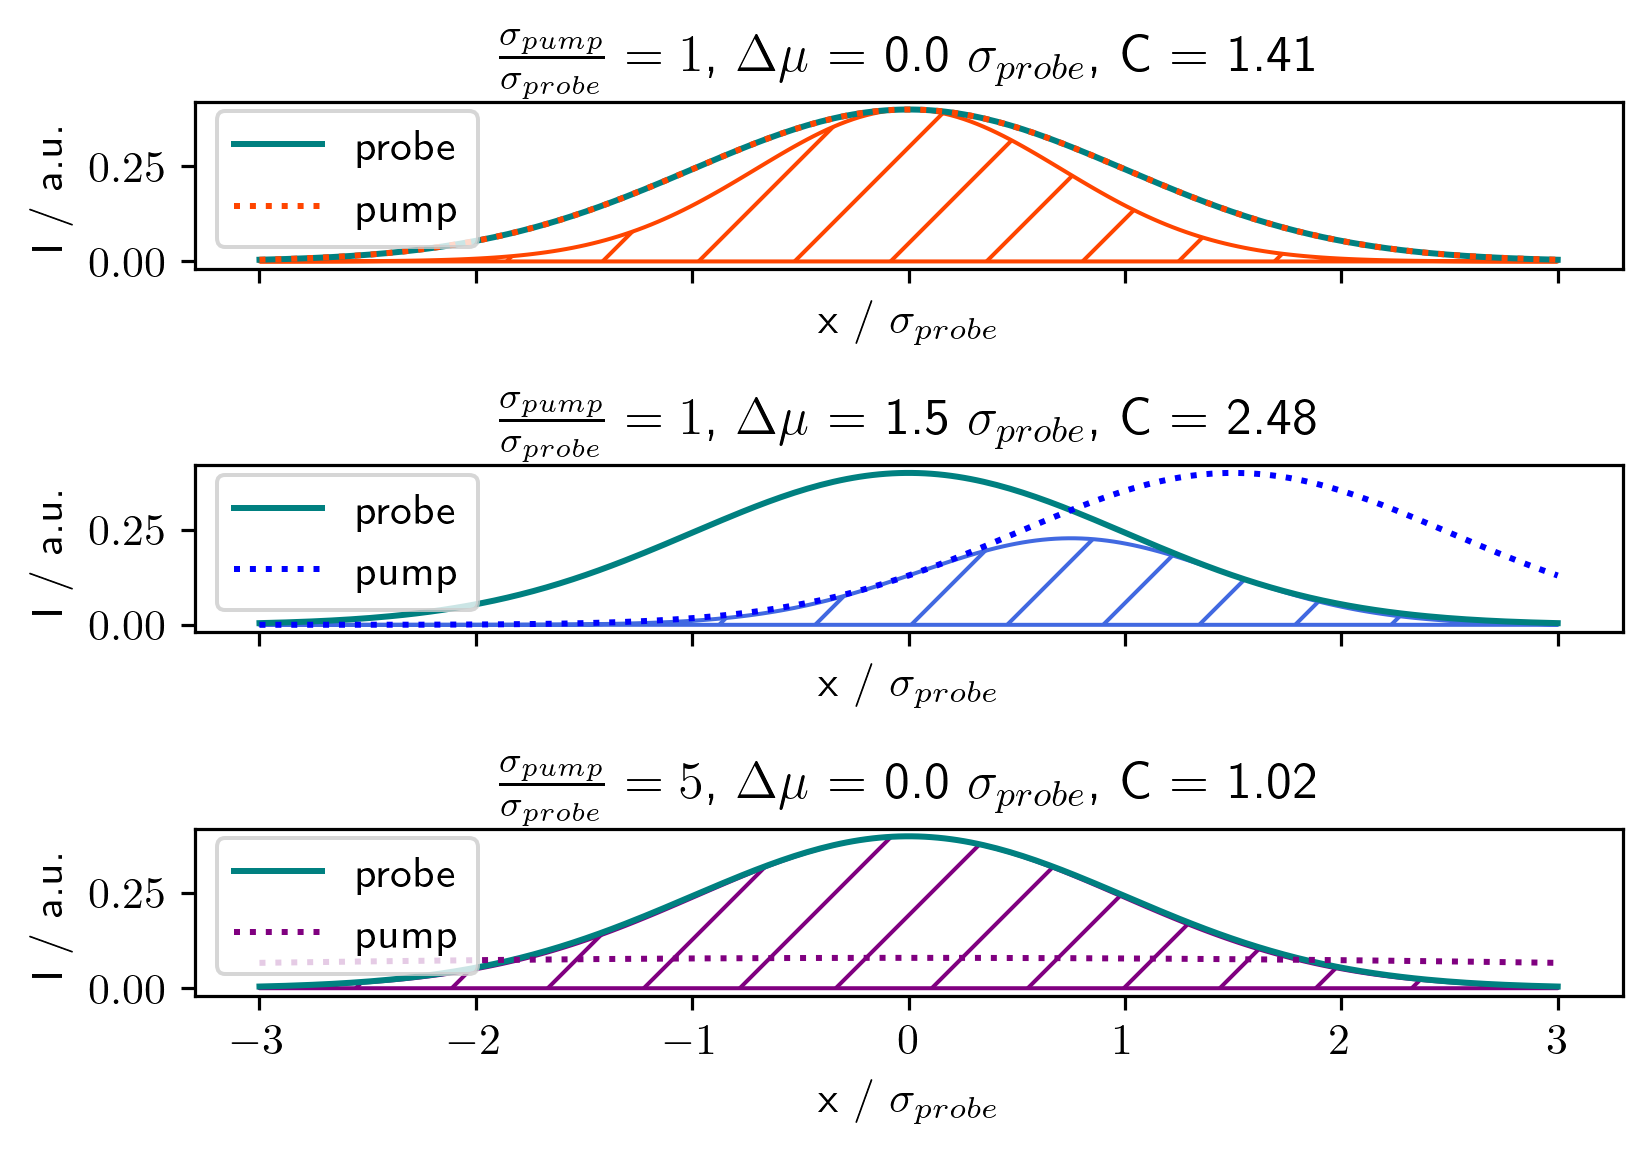
\includegraphics[scale=1]{images/OverlapVisualisationProbeSelection.png}
\caption[Selection of probe point spread function based on spatial pump-probe overlap.]{Selection of probe point spread function based on spatial pump-probe overlap. C is the correction factor calculated according to section eq. \ref{eq:fullCorrectionFactor}. Hatched area shows the weighting of the probe happening due to linear pump power dependence of transient response.\label{fig:overlapVisualisation}}
\end{figure}

\section{Degradation compensation}
The samples used show a reduced response over increasing exposure times to the pump and probe beams. A simple dose related model is used in eq. \ref{eq:degradationIntroduction}, where $\Delta A(t)$ is the response, $t$ is the total exposure time of the sample spot, $\tau_{1/e}$ is the degradation time constant where the response falls to 1/e and $I_{\mathrm{peak}} = f_{rep}\cdot \radiantExp$ is the average peak radiant exposure per second or irradiance.

\begin{equation}\label{eq:degradationIntroduction}
\Delta A(t) = \Delta A(t_0)\cdot e^{-\frac{(t-t_0)}{\tau_{1/e}}\cdot f_{rep}\cdot \radiantExp}
\end{equation}
A detailed look at data, along with reasoning to why this model is used, is shown in sec. \ref{sec:degradation}.

\section{Sample variation correction}
Due to sample inhomogeneities  the response varies over the sample area surveyed. It is attempted to correct for this by first measuring a grid like map of the sample at a known GSD probe wavelength, here pump \qty{653}{\nano\meter} probe \qty{680}{\nano\meter} were chosen. Related measurements are then multiplied with a relative factor, to normalise their response. This should be a valid approach for pump radiances below threshold for non-linear processes, when avoiding impurities.

\section{Background subtraction}
All measurements have a constant background, offsetting the measurement ahead of pump and probe temporal overlap, meaning the probe pulse passing through the sample ahead in time of the pump pulse. This is mainly due to stray light or sample fluorescence of the pump reaching the detector.  A correction is made by shifting the ${\frac{I_\text{pump-probe}}{I_\text{probe\, only}}}$ in such a way, that it is 1 ahead of the temporal overlap point. \\
However sometimes a linear component, for example from minor pump movement due to imperfections of the stage along its travel, is observed. If the linear component is small enough it may similarly to a static offset be corrected by a linear fit of the ratio ${\frac{I_\text{pump-probe}}{I_\text{probe\, only}}}$. Once the component is too large a measurement has to be considered faulty. Depending on how large the linear component is decay constants may not be viable, however the immediate response after temporal overlap may be considered correct after subtracting the linear component.\\

Theoretically the correct way of applying a background subtraction, under assumption that it indeed only is stray pump light, would be to only subtract the background from ${I_\text{pump-probe}}$. This is not possible however, due to temporal variations in probe intensity, which cancel for the ratio ${\frac{I_\text{pump-probe}}{I_\text{probe\, only}}}$.



\chapter{Beam Characterisation and Correction}\label{chp:OverlapCorrection}
In this chapter the reasoning and methods to characterise the beams, as well as the absorbance correction for their overlap, is introduced.

\section{Overlap compensation}
Opposed to the regular setup, where the achromatic objectives guaranteed relatively consistent overlap of pump and probe, the UV setup has the need to correct the overlap variation between single measurements, since the refraction of the dispersive elements in the probe path varies strongly in the UV range and any compensation via the telescope will be imperfect.\newline
Relevant for this are the beam sizes as well as the overlap of the pump and the probe beam in the sample as described in sec. \ref{sec:overlapCorrDescription} and shown in fig. \ref{fig:overlapVisualisation}. Variations in those parameters are induced by change of the beam-shape due to second harmonic generation, imperfect alignment of the SHG telescope and correction of the chromatic aberration for different wavelength settings of the probe. The full description of the correction factor is below in sec. \ref{sec:CorrFactor}.\\

The characterisation of the beam shapes during the measurement procedure is currently done with a simplified fitting routine in C\#, detailed in sec. \ref{sec:LiveFitting}, to allow setting the overlap and record the images directly from live camera data. The second step of calculating the correction factors for the measurements is done with a python class that loads raw saved camera data and has more analysis options. The basic use of the python class is briefly introduced in sec. \ref{sec:pythonBeamCharacterisation}.

\subsection{Correction factor}\label{sec:CorrFactor}
The correction factor aims to equilibrate the transient absorbance of the given \text{pump-probe} overlap to an ideal state, where the pump is constant in irradiance over the entire probe area or assuming Gaussian intensity distributions is infinitely larger than the probe beam. This would allow the entire probe distribution to experience the same change in absorption.
Thus for very high $\mathrm{\frac{\sigma_{Pump}}{\sigma_{Probe}} \rightarrow \infty}$ the correction factor has to tend to 1, which is the smallest value.
%The factor is calculated from the Gaussian intensity distributions as seen in eq. \ref{CorrFactorGaussians}, of which the derivation is shown in section \ref{GaussiansDerivation} or in Bromiley\cite{Bromiley2014}, which was used to check correctness. The enumerator is the integral over essentially the probe intensity with the constant factor of the maximum pump intensity 
Considering this, the correction factor $C$ is chosen as the integral over the product of the ideal pump, an infinite plateau, with the Gaussian probe. The denominator on the other hand is the integral over the actual product of the Gaussian fits of pump and probe beam.  
\begin{equation}\label{eq:CorrFactorGaussians} 
C = \dfrac{\int I_\text{pump}^*(x)\cdot I_\text{probe}(x) \;dx}{\int I_\text{pump}(x)\cdot I_\text{probe}(x) \; dx} = \dfrac{c^*\cdot \int I_\text{probe} dx}{S_{12}} = \dfrac{c^*}{S_{12}}
\end{equation}
The ideal top-hat pump distribution power is chosen to be the peak of the Gaussian power distribution of the real beam $\mathrm{max}\left(I_{pump}(x)\right)$. This means choosing the factor according to the geometry of the true pump beam as defined:
\begin{equation*}\label{eq:maxPowerGauss}
I_\text{pump}^*(x) = c^* = max(I_\text{pump}(x)) = \frac{1}{\sqrt{2\cdot\pi}\cdot\sigma_\text{pump}}
\end{equation*}

$\mathrm{S_{12}}$ is defined in eq. \ref{eq:S12CorrectionFactor} and serves as the extra normalisation factor for rewriting the product of the two Gaussians into a single Gaussian. The derivation of the single Gaussian can be seen in sec. \ref{deriv:GaussiansDerivation} and has been cross-checked with Bromiley.\cite{Bromiley2014}

\begin{equation}\label{eq:S12CorrectionFactor}
S_{12} = \dfrac{1}{\sqrt{2\pi\left(\sigma_1^2+\sigma_2^2\right)}}\cdot exp\left(-\dfrac{\left(\mu_1 - \mu_2\right)^2}{2\cdot \left(\sigma_1^2+\sigma_2^2\right)}\right)
\end{equation}

Combining eq. \ref{eq:S12CorrectionFactor} and eq. \ref{eq:CorrFactorGaussians} gives the full correction factor C:
\begin{equation}\label{eq:fullCorrectionFactor}
C = \sqrt{\frac{\sigma_1^2+\sigma_2^2}{\sigma_1^2}}\cdot exp \left(\frac{\left(\mu_1-\mu_2\right)^2}{2\cdot \left(\sigma_1^2+\sigma_2^2\right)}\right)
\end{equation}

A few illustrations of the behaviour of the correction factor are shown in fig. \ref{fig:overlapVisualisation}. Furthermore to have all relative $\Delta A$ values be directly comparable, the correction factor is divided by the pump radiant exposure $\radiantExp$ in practice. This accounts for the correction factor itself only considering the normalised Gaussian beam shapes. The product of the individual correction factors for both pixel axes is the total correction factor.

\begin{table}[h]
\caption{Illustrative one dimensional correction values for fitted Gaussians.}
\centering
\begin{tabular}{c|rrrrrr}\toprule
$\Delta \mu$ / $\sigma$                     & 0          & 0             & 0              & 0             & 1              & $2\cdot\sqrt{2 ln(2)}$ \\
$\dfrac{\sigma_\text{pump}}{\sigma_\text{probe}}$ / 1 & 1          & 3             & 2              & 1/2           & 1              & 1                      \\
Correction Factor                           & $\sqrt{2}$ & $\approx1.05$ & $\approx 1.12$ & $\approx 2.24$ & $\approx 1.82$ & $\approx 5.66$ \\ \bottomrule       
\end{tabular}
\end{table}


To ascertain how well this works a numeric variant of the correction factor is considered based on the same principle as eq. \ref{eq:CorrFactorGaussians}:
\begin{equation}\label{eq:correctionNumeric}
C_\text{numeric} = \sum_{i=0}^{N_x}\sum_{k=0}^{N_y}\frac{max\left(I_\text{pump}\right)\cdot I_{probe}(x_i,y_k)}{I_\text{pump}(x_i,y_k)\cdot I_\text{probe}(x_i,y_k)}
\end{equation}
where ${x_i/y_k}$ are discrete points, which may be associated with single pixels of the camera, of which there are $N_x$ for $x_i$ and $N_y$ for $y_k$. $max\left(I_\text{pump})\right)$ once again is the maximum value of ${I_\text{pump}}$ over all ${x_i, y_k}$. 

Comparing the numeric approach with the analytic fitting approach is done by generating a hypothetical pump and probe Gaussian pair, for which the correction factors are calculated. A discrete map of size $\pm 5\cdot \sigma_\text{max}$ with a point density of $2^{10}\, \frac{\text{points}}{\sigma_\text{max}}$ is used. The analytic value is generated directly from the generating parameters for the numeric discrete map. For $I_\text{pump} = \text{const}$ the correction factor trivially goes to one as per definition. Since the discrete values strongly depend on the number of bins an approach is chosen, where a density of discrete points per $\mathrm{\sigma}$ of the generating Gaussian distribution is shown. Interpolating the binned points linearly shows an improvement for low discrete point densities per $\sigma$, however is very similar to pure summation at higher point densities. Linear interpolation was chosen to avoid unexpected behaviour of spline fitting. To visualize this the correction factor of a pump and probe combination, where $\mathrm{\sigma}$ and $\mathrm{\mu}$ are identical for both distributions, is shown over a number of bin sizes in fig. \ref{fig:NumericalCorrectionSNR}. Integer multiples of two pixels or discrete points, in each axis, are binned together and the bins are kept square in size. The influence of a noise component, uniformly distributed for a specific signal to noise ratio (SNR), is also shown. The noise is added onto each Gaussian map individually.

\begin{figure}[h]
\centering
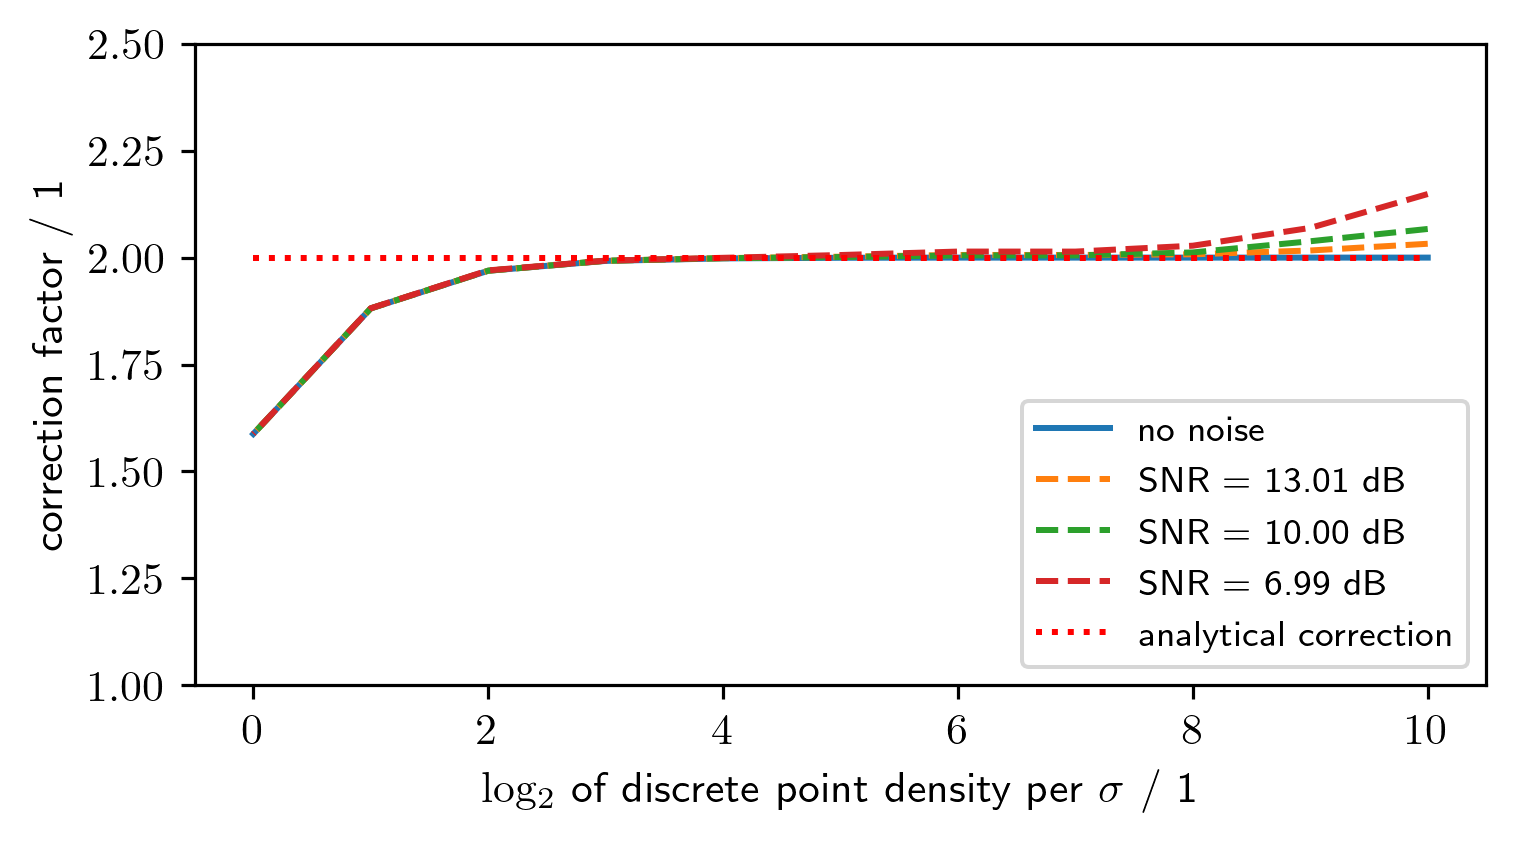
\includegraphics[scale = 1]{images/NumericalCorrectionSNR_interpolation.png}
\caption[Comparison of numerical and analytic correction factors for radial-symmetric Gaussian distributions of identical parameters.]{Comparison of numerical and analytic correction factors for radial-symmetric Gaussian distributions of identical parameters. For the SNR graphs a random, uniformly distributed, noise was added to both Gaussian maps individually. A linear interpolation of $2^4$ points per $\sigma$ is used for discrete bin densities up to, including, $2^4$ points per $\sigma$. Above this density threshold a direct summation without interpolation is done according to eq. \ref{eq:correctionNumeric}.\\$\frac{\sigma_\text{pump}}{\sigma_\text{probe}}=1$, $\Delta\mu = 0$\\\label{fig:NumericalCorrectionSNR}}
\end{figure}

To check for possible effects regarding an offset of the center position from the pixel grid and breaking the radial-symmetry, the Gaussian distributions are now shifted by 1 $\mathrm{\sigma}$ in both x and y direction from each other in fig. \ref{fig:NumericalCorrectionShift}. Furthermore both distributions are incrementally shifted together, by an offset from the pixel grid in x direction. Doing this incremental shift in both x and y direction leads to a small change for the point densities that are close to the analytic correction factor. 

\begin{figure}[h]
\centering
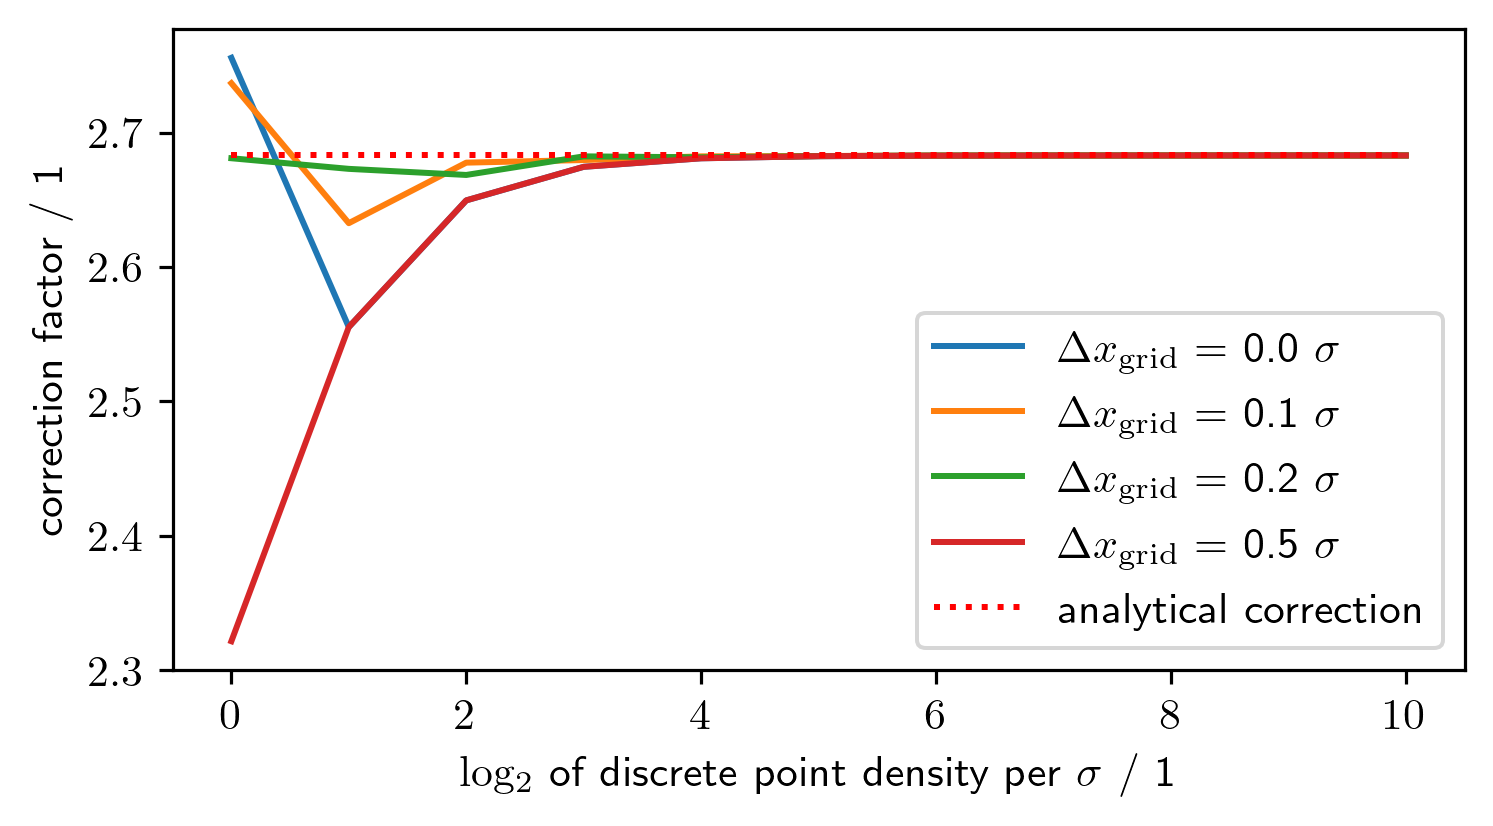
\includegraphics[width=0.9\linewidth]{images/NumericalCorrectionShiftedBeams_interpolation.png}
\caption[Comparison of analytic and numeric overlap correction factor with varying shift of point spread functions regarding simulated pixel grid in x direction.]{Comparison of analytic and numeric overlap correction factor with varying shift $\Delta x_\text{grid}$ of point spread functions regarding simulated pixel grid in x direction. A linear interpolation of $2^4$ points per $\sigma$ is used for discrete bin densities with up to, including, $2^4$ points per $\sigma$. Above this density threshold a direct summation without interpolation is done according to eq. \ref{eq:correctionNumeric}.
\\$\frac{\sigma_\text{x-pump}}{\sigma_\text{x-probe}}=0.8;\frac{\sigma_\text{y-pump}}{\sigma_\text{y-probe}}=2.0;\Delta\mu_\text{total} = \sqrt{2}; \Delta\mu_{x} = \Delta\mu_y = 1$\label{fig:NumericalCorrectionShift}}
\end{figure}

With the front camera as it is, the actual sample density of the point spread function is in the range of 2 to 4 $\frac{\text{px}}{\sigma}$, which does not seem sufficient to avoid the fitting process and do the correction factors strictly numerically, including the linear interpolation of points, when comparing to the pixel density $\mathrm{log_2(4) = 2}$ in fig. \ref{fig:NumericalCorrectionSNR} and fig. \ref{fig:NumericalCorrectionShift}. Note that with

\subsection{Beam characterisation}\label{sec:pythonBeamCharacterisation}


The python class ArtFit has some options to check for the validity of the data used. Since data is currently saved as a region of interest (ROI) compared to the background, which is the entire sensor, ROI parameters are needed. Before version 1.3 of "ArtrayLiveFitC\#" data is saved in a raw format without metadata, meaning ROI parameters had to be recorded manually.  The beam shape is saved as a raw file corresponding to the ROI set in LiveFit. With version 1.3 of ArtrayLiveFitC\# XML files with the raw data encoded in base64 are used to also pass metadata, including the ROI. This removes the need to manually note ROI and other parameters.\\
ArtFit version 1.3 may parse 3 different input types:
\begin{enumerate}
\item Quick plotting of raw data:\\
With a path to a raw data file and an optional boolean value, which is used to tell the program to use the standard size of 1280x720 instead of a square pixel array size deduced from total number of entries. Plots the beam intensity profile without any processing. If using XML the size is taken from the metadata.
\item Single beam profile with background subtraction: \\
Loads a JSON with metadata for background subtraction, the path for the beam profile to be loaded and a width for fitting. Using XML overwrites the ROI given by the JSON metadata.
\item Two beam profiles with background subtraction: \\
ROI offset has to be identical and is again defined by a JSON file with background location. JSON position parameters again ignored if using XML starting in version 1.3.
\end{enumerate}

To get meaningful data for correction of data the pump power has to be set using setPumpPower() and the $\mathrm{\frac{\si{\micro\meter}}{px}}$ scale can optionally be overwritten from the background file with setScale(). Fitting is done by calling plainFit($id$), where $id$ = 1 for probe (first filepath handed over) and $id$ = 2 for pump (second filepath).

Some options to show the images as well as the fits are:
\begin{itemize}
\item plotComp()\\
Shows an intensity contour plot of both beams on top of each other. If only one beam file is loaded only one is shown. Also shows the fitted intensity slices on top of each other for both pixel array axes. Returns an overlap estimator corresponding to what is given by the liveFitting program described in section \ref{sec:LiveFitting}. See example in fig. \ref{fig:plotComp}.
\item plotGauss()\\
Plots the intensity profile of the beams, if both are given, separately with an overlayed contour plot of the fits, to ascertain the validity of the fit. Needs to have already fitted data with plainFit() to show the Gaussian distribution. Fitted data may be printed to console by setting printData = True for the options. The intensity profile is shown by default without background subtraction and can be shown with subtracted background by handing over a boolean. The fits are always done with subtracted background, the profile just is not shown background subtracted by default. See example in fig. \ref{fig:plotGauss}.
\end{itemize}

\begin{figure}[hbtp]
\centering
\begin{subfigure}[t]{0.49\linewidth}
\centering
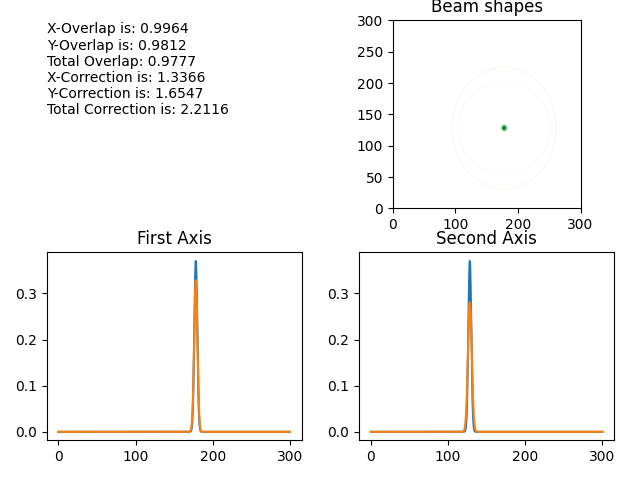
\includegraphics[width=\columnwidth]{images/ArtrayExamplePics/ArtFit_PlotComp.png}
\caption{PlotComp(): Beamshapes are plotted as fitted contours and fitted overlap is shown one dimensional for each axis. Top left the overlap as defined in ArtrayLiveFitC\# and the correction factor according to ArtFit is shown for individual axes and the total product.\label{fig:plotComp}}
\end{subfigure}
\hfill
\begin{subfigure}[t]{0.49\linewidth}
\centering
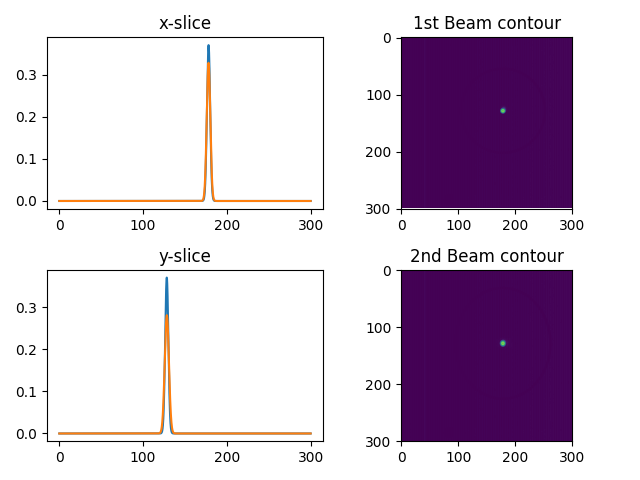
\includegraphics[width=\columnwidth]{images/ArtrayExamplePics/ArtFit_PlotGauss.png}
\caption{PlotGauss(): Left are the one dimensional fitted overlaps shown for each axis and on the right the raw data map along is shown with an overlay of the fitted beamshape as a contour.\label{fig:plotGauss}}
\end{subfigure}
\caption{Example images of ArtFit graphic output.}
\end{figure}



\subsection{ArtrayLiveFitC\#}\label{sec:LiveFitting}
As the Artray $\mathrm{ARTCAM-092UV-WOM}$ could not be interfaced with matlab using the webcam library a C\# program was created based on the manufacturers example program.\cite{Artray2018}
Issues with our system are, that for our specific camera or system setup, a periodic variation of low intensity signal is reported by the C\# based program, while this periodic variation is missing in the official ART-MEASURE software. Attempts were made to troubleshoot this in correspondence with the manufacturer, who were very forthcoming in the matter, but it could not be solved so far. To overcome this problem a simple reference-image background-subtraction has been devised as sufficient, as the variation seems to be constant over time. The background has been recorded with the lens cap on at an exposure of 15 ms, which was chosen after comparing the quality of background subtracted output for 0.3 ms, 15 ms and 100 ms exposure. 
\newline
For all measurements included here version 1.2 of ArtrayLiveFitC\# was used. The ALGLIB\cite{Bochkanov2024} software package is used for fitting a Gaussian to the beamshape. ScottPlot 4\cite{ScottPlot4} is used to display the fitted data.\\
\subsubsection{Fitting principle}
In version 1.2 the relevant fitting parameters are returned along with a numeric overlap integral based on the Gaussian beam shapes. Starting with ArtrayLiveFitC\# version 1.3 it has been rebased into an analytical form as per eq. \ref{eq:GaussianProduct}, which describes the simple product of two Gaussians.
\begin{equation}
\mathrm{overlap} = \int \sqrt{f_1(x)\cdot f_2(x)}dx =  \sqrt{\frac{2 \sigma_1^2\sigma_2^2}{\sigma_1^2+\sigma_2^2}}\cdot exp\left(-\frac{\left(\mu_1-\mu_2\right)^2}{4\cdot \left(\sigma_1^2 + \sigma_2^2\right)}\right)\label{eq:GaussianProdcut}
\end{equation}
This is calculated separately for both axes of the pixel array and then multiplied for a final value. 
This is not directly related to correction factor calculated within the python program ArtFit used to make individual measurements comparable, but is more of a measure of how similar the beams are, which is why only the normal distributions are used without an intensity modifier, thus both beams are weighted identically. \\
This is reasonable as the best results for the correction factor, for the Artray camera pixel density, are achieved when pump and probe beams are similar in size, with a preference for a smaller probe beam shape. This overlap integral returns a maximum value of 1 when the beams are identical. It falls off quickly if the intensity maxima are shifted and slowly if the FWHM of the beams is different.\\
\subsubsection{Operation}
Before startup all needed DLL files need to be in the same directory as the executable.\footnote{alglib.net.dll, ArtCamSdk\_092UV\_WOM.dll, ScottPlot.dll, "ScottPlotWinForms.dll", Python.Runtime.dll,...} Additionally .NET Framework 3.5 is required. Upon startup the program should automatically connect to the camera. Otherwise check the dll and device submenus.
The main forms shown upon startup are the camera control form in fig. \ref{fig:ArtrayMain} and the fitting form in fig. \ref{fig:ArtrayFitting}.

\begin{figure}[hbtp]
\centering
\begin{subfigure}[t]{0.49\linewidth}
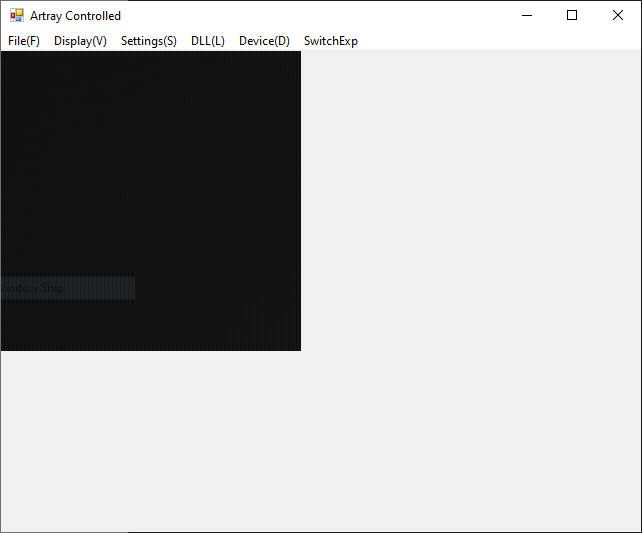
\includegraphics[width = \columnwidth]{images/ArtrayExamplePics/ArtrayControlledMain.PNG}
\caption{"Artray Controlled" window.\label{fig:ArtrayMain}}
\end{subfigure}
\hfill
\begin{subfigure}[t]{0.49\linewidth}
\centering
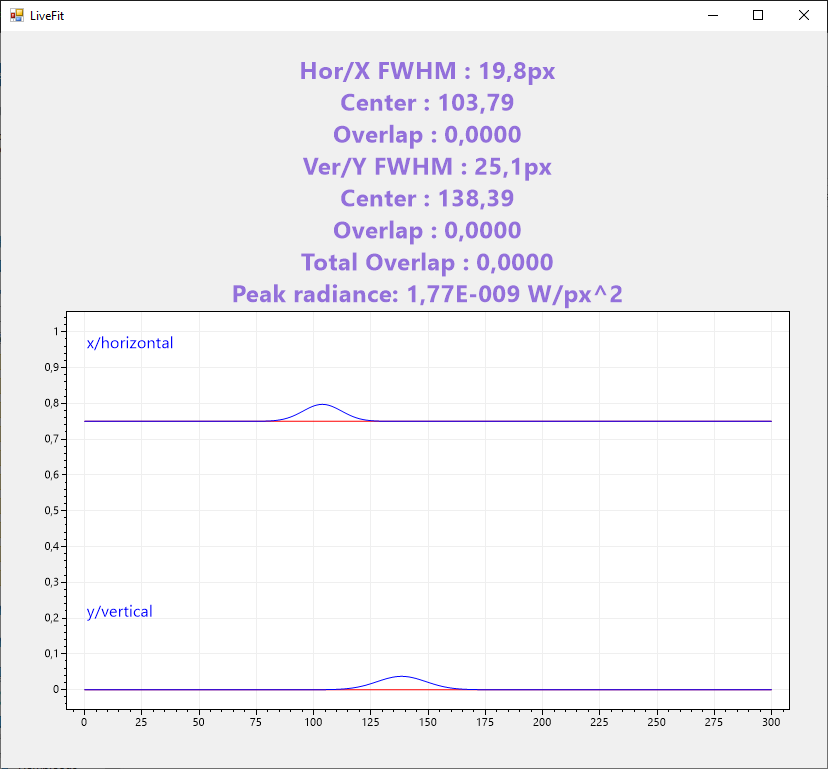
\includegraphics[width = \columnwidth]{images/ArtrayExamplePics/FittingForm.PNG}
\caption{"LiveFit" window. Scottplot 4\cite{ScottPlot4} is used to generate the output for this figure.\label{fig:ArtrayFitting}}
\end{subfigure}
\caption{Control and data display forms for setting and acquiring overlap measurements from Artray camera.}
\end{figure}


To get an image there are several options in the "Display" drop down menu.
\begin{itemize}
\item Preview: starts a livestream within the "Artray Controlled" window.
\item Snapshot: records a new frame and statically shows it. If possible a fit will be shown in the "LiveFit" window.
\item Callback: starts a livestream with periodic fitting. Preview should be preferred if no fitting is needed or possible for performance reasons, such as when the ROI is very large.
\end{itemize}

To adjust the image parameters or camera settings use the "Settings" drop down menu.
\begin{itemize}
\item Camera settings: opens a menu to set the image format including size and ROI as well as color format, which is to be set to "Color 48bit *" for reasons that are explained in the external software description for the Artray camera interaction.\cite{Jeindl2024} The effective ROI should be set to 300 pixels vertically and horizontally. The ROI should stay square and not rectangular, as there is a bug preventing correct data manipulation at this moment. An example of the settings can be seen in fig. \ref{fig:artrayCameraSetting}.
\item Filter settings: include software settings for brightness, contrast, saturation etc. Influence of "Bayer Mode" on the monochromatic sensor is unknown, as it does not show an obvious difference in output. Keep the saturation at -255.
\item Analog settings: consist of gain and exposure. Also has the option to mirror the image vertically and horizontally, which should not be done after calibration. Before ArtrayLiveFitC\# version 1.3 there is no way of telling from raw output data at, which setting a snapshot was taken at.
\item Misc: is where custom settings for output parameters as well as exposure can be set. Assigning a "µm per px" value and adjusting the power correctly allows a readout  of directly corrected peak radiance and other fit parameters such as the FWHM. The three exposure values can be quickly jumped to from a drop down menu "SwitchExp" in the main window and are supposed to help streamline the measurement process. The menu can be seen in fig. \ref{LiveFitting:MiscMenu}.
\end{itemize}

\begin{figure}[hbtp]
\centering
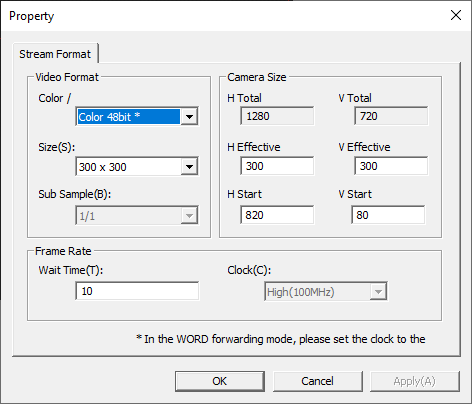
\includegraphics[width = 0.6\linewidth]{images/ArtrayExamplePics/StreamProperties.PNG}
\caption{Menu for camera settings given by Artray. Example settings to get good data output within a square ROI.\label{fig:artrayCameraSetting}}
\end{figure}

\begin{figure}[hbtp]
\centering
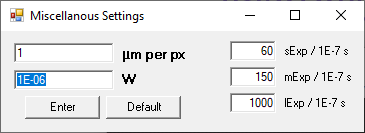
\includegraphics[scale=1]{images/ArtrayExamplePics/DefaultMiscSettings.PNG}
\caption[Miscellaneous menu for setting quick change exposure values and additional constants to correct fitting output.]{Miscellaneous menu for setting quick change exposure values and additional constants to correct fitting output. 
Default value of "µm per px" means that the fitting form shows the FWHM and related values in units of pixels. The exposure values are in 0.1 µs steps, as this is what the camera allows. Only integer input is supported for these exposure settings.\label{LiveFitting:MiscMenu}}
\end{figure}



As mentioned quick swap exposure settings can be set. They are accessed from the drop down menu "SwitchExp". Upon switching exposure a snapshot is taken, this interrupts all other image acquisition types, and a maximum pixel intensity is reported in a pop up window, to show if the dynamic range of the camera is being used well. If that is not the case the fitting window either turns \textcolor{blue}{blue}, if the exposure is too low (30\% of 12 bit), or turns \textcolor{red}{red}, if it is too high (95\% of 12 bit). Setting exposure can sometimes be slower than readout of the snapshot, thus reporting a value ahead of setting the new exposure value. If that is the case just set exposure again if one wishes to get the maximum pixel intensity value.\\

The file drop down menu consists of features for saving, opening and comparing data:
\begin{itemize}
\item Save: saves a raw txt file of the last captured image. In case of a livestream this is the last shown image. For a snapshot it saves the currently shown snapshot. Starting with ArtrayLiveFitC\# version 1.3 an XML with metadata is saved; the binary data being encoded in base64.
\item End: Ends the program. (Removed in ArtrayLiveFitC\# version 1.3 as forms may be closed intuitively.)
\item Reference: sends a reference image, behaviour is like with save regarding livestreams, to the "LiveFit" window. There a fit of the reference is shown as a red graph, which when not set is flat.
\item Open: works like reference, however it opens the reference snapshot from a raw ".txt" or ".xml" file of choice via file dialogue.
\item Background: sets a background to subtract from the images for live fitting. Setting background does not alter the behaviour of Save. Saved files are still plain raw unaltered data from the sensor. The background file location is automatically loaded when starting a session and is saved in the windows registry under $\mathrm{"Computer \backslash HKEY\_CURRENT\_USER \backslash SOFTWARE \backslash LiveFit"}$ as \text{"BACKGROUND\_FILE"}. The LiveFit subkey needs to be created manually, possible with regedit, ahead of first use. The BACKGROUND\_FILE subkey is automatically added and handled by the program.
\end{itemize}


\chapter{SQIB in PMMA}\label{chpt:results}
In this chapter the main results, a wavelength scan of extended wavelengths, are presented and details of the sample are discussed. The motivation was to find excited states, at higher energy than previously reported, to use for modelling purposes. Other than an extension of the falloff of the ESA peaks and a \textbf{qualitative} reproduction of peak positions of Zheng et al\cite{Zheng2020}, no further peaks could be defined.

\section{1wt\% SQIB in PMMA matrix}
The sample is 1wt\% SQIB in a PMMA solid solution provided by Manuela Schiek\footnote{Sample No. 4 from 2021}. The sample is not annealed and shows fluorescence if illuminated by white light, implying the influence of neighbouring molecules is not strong enough to quench the fluorescence at this concentration. \\

It is assumed that the relatively fixed structure of the squaraine hinders structural rearrangement within the rigid PMMA matrix.
Opposed to liquid solutions like $\mathrm{CHCL_3}$, no quick solvent reorganisation for n-butyl terminated squaraine molecules within PMMA was observed by Zheng et al.\cite{Zheng2020}, for squaraines with side chains of similar bulkiness. This makes it unlikely for our sample to have such solvent reorganization in PMMA either.

An average nearest neighbour distance for this concentration may be taken as \SI{2.36}{\nano\meter} according to Zheng et al.\cite{Zheng2020}, who based the calculation on poisson statistics\cite{Krider2003}. The actual spread of nearest neighbour distances is an extended distribution. Thus there is an expectation of some quenching of effects, such as quenching of fluorescence and decay times of excited states. However with the bulk of the molecules being at larger distances these effects should be virtually unobserved.\cite{Zheng2020} \\
Collective effects like Davydov splitting, which are dependent on a relative orientation of transition dipole moments of subunits, are negligible for SQIB samples at this concentration, which are not annealed, and are not observed as the average distance is great enough.\\

\begin{figure}[!htp]
\centering
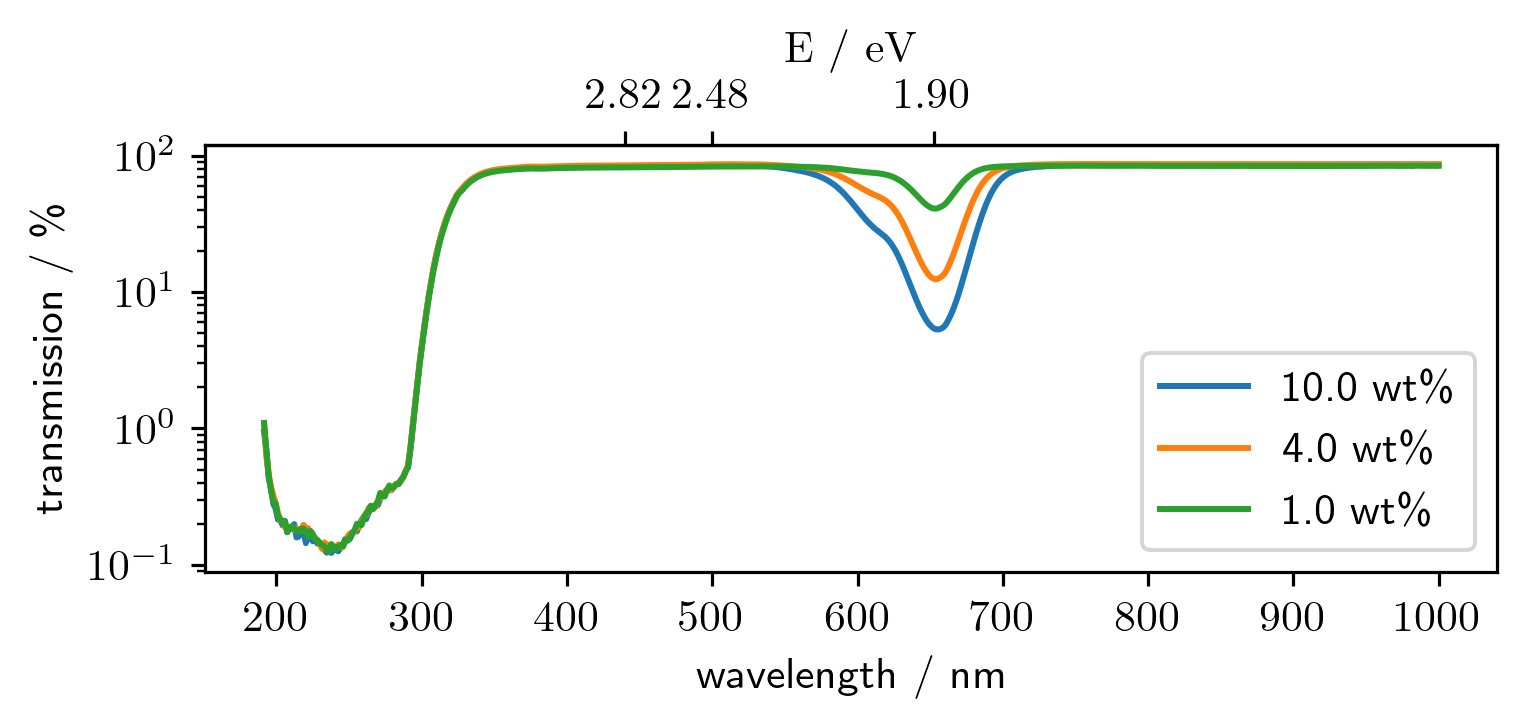
\includegraphics[scale = 1]{images/SQIB_VarPercentInPMMA_transmission.png}
\caption[Continuous wave transmission spectrum of the varying percentages of SQIB in PMMA samples.]{Continuous wave transmission spectrum of the varying percentages of SQIB in PMMA samples.\label{fig:VarpercentCWspectrum} Preliminary CW transmission spectrum of the SQIB in PMMA by Manuela Schiek 2022.\cite{Schiek2022} Reference sample with PMMA has a film thickness of roughly \SI{650}{\nano\meter}}
\end{figure}

As shown in the spectrum in fig., \ref{fig:VarpercentCWspectrum} the main CW absorption feature of isolated SQIB itself is at 653 nm. Increasing the concentration and thus introducing collective effects causes a widening of the absorption feature towards 600 nm. Due to the absorption of glass and the PMMA matrix itself taking over below 300 nm no measurements below 300 nm were made.\\

\section{Wavelength dependence of 1wt\% SQIB in PMMA}


Even though the sample is intended to be relatively homogeneous, there are variations in sample response over the area surveyed. For wavelength scans shown in context of the SHG setup, sample spots without strong variations in the vicinity were preferred. See example in fig. \ref{fig:plotGauss}. Variation of the sample response at different measurement points is accounted for as a factor normalised by the mean sample response for a pump 653 nm probe 680 nm combination. The mean response is taken from the mean of all measurements used. Uncertainty estimation is unavailable due to limited resolution of the map. Resolution is limited due to high time expense of mapping the sample area. Since exposure of single spots is rather short, no discernible sample degradation is expected from these mapping operations. The map used for correction of the shown wavelength scans may be seen in fig. \ref{fig:TA_image_sample}. Pump power before and after measurement are identical, however probe power varied over time.\\
Also applied is the overlap correction factor with a fitting width using a 3 px average centered on a peak fit. Degradation compensation is applied, as described in sec. \ref{sec:degradation}, using the same $\tau_{1/e} = \SI{12600}{\second}$ time constant corrected for the pump single-shot radiant exposure $\radiantExp$ used in the measurement.
Measurements are done only in parallel pump and probe polarization.\\

\begin{figure}[hbt]
\centering
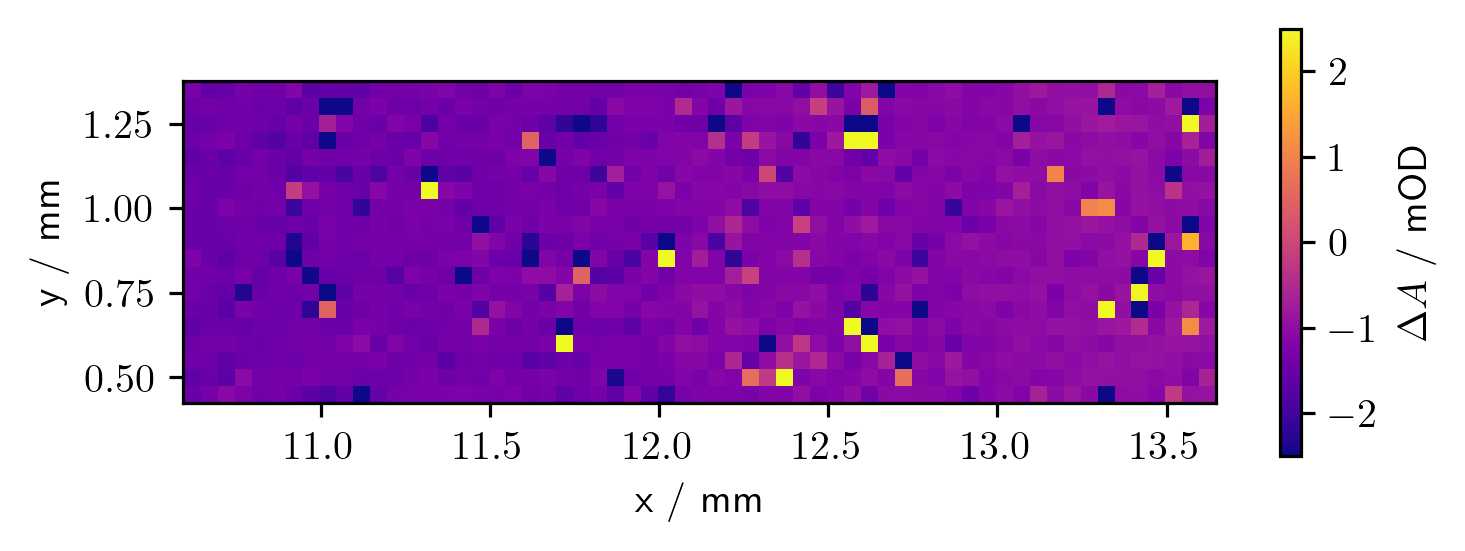
\includegraphics[scale=1]{images/1percentSQIBinPMMA_Sample653-680Image.png}
\caption[Transient absorption image of 1wt\% SQIB in PMMA sample from image\_0245 with subtracted background image\_0244 for pump \qty{653}{\nano\meter} and probe \qty{680}{\nano\meter}.]{Transient absorption image of 1wt\% SQIB in PMMA sample from image\_0245 with subtracted background image\_0244 at a probe spot size of approximately \SIrange{36}{45}{\micro\meter} FWHM. Colourmap is truncated at $\pm2.5\,\text{mOD}$.\\ Extreme deviations from mean transient absorbance are likely to be imperfections in or on the sample and have to be avoided for measurements.\\ Pump peak radiant exposure at \SI{653}{\nano\meter} $\radiantExp\approx$ \pumpExp{82e-3}, probe radiant exposure at \SI{680}{\nano\meter} $\radiantExp\approx$\SIrange{7.9e-3}{12.6e-3}{\radExp}\frep{40} \label{fig:TA_image_sample}}
\end{figure}

The transient behaviour of the sample is shown in fig. \ref{fig:SQIB_PMMAwavelengthscan}, where fitted delay points are shown to see the immediate transient behaviour. They are fitted using a nonlinear curve\_fit from scipy.optimize to fit eq. \ref{eq:transientDecay}. The number of exponential components may be automatically determined by fitting, however within this thesis they are set by hand to achieve best fitting. An example for a fitted delay scan is seen in fig. \ref{fig:delayFitExample}.
\begin{equation}\label{eq:transientDecay}
f(t) = \left[\sum_{n=0}^{n_\text{max}} \Delta A_n\cdot exp \left(\frac{-(t-t_0)}{\tau_n}\right)\right]\cdot \int_{-\infty}^t exp\left(-\frac{(t-t_0)^2}{2\sigma^2}\right)
\end{equation}

\begin{figure}[hbtp]
\centering
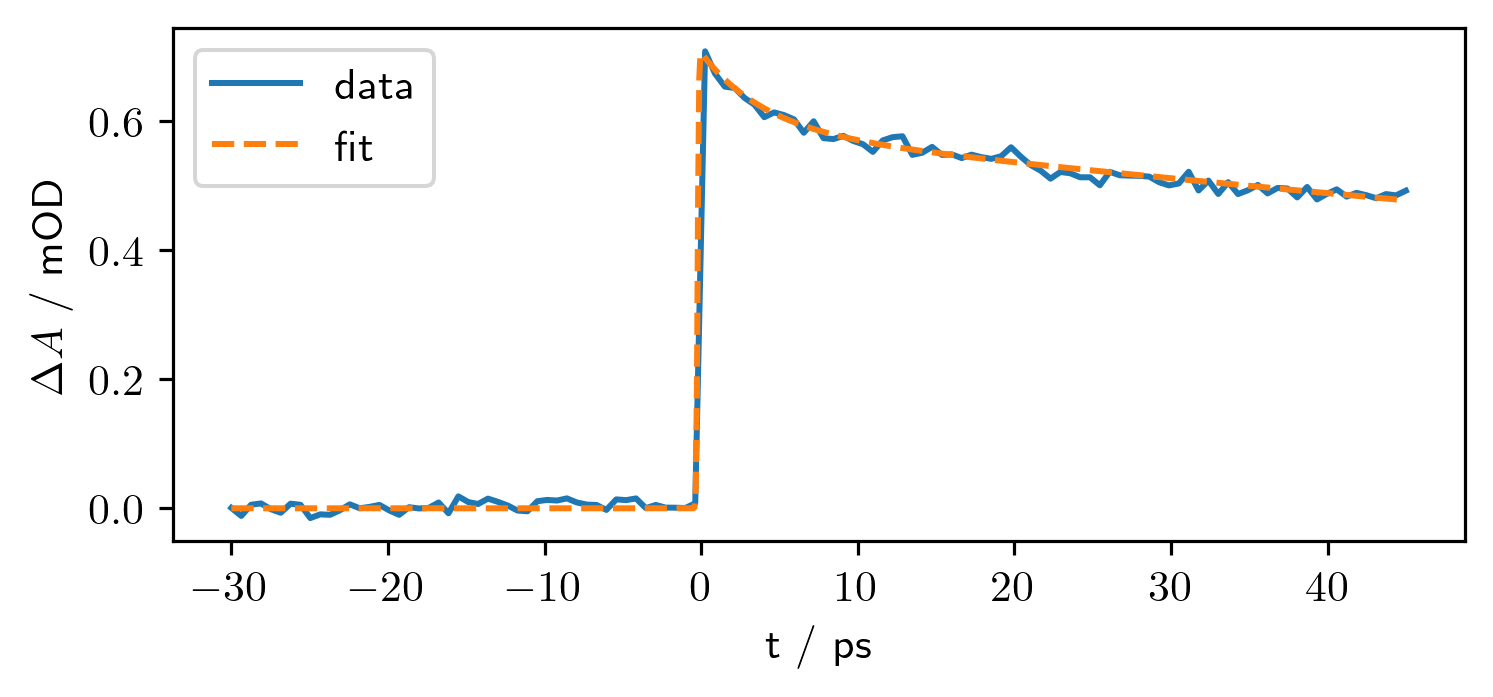
\includegraphics[scale=1]{images/ExemplaryDelayScanFit_Pump653Probe493.png}
\caption[Exemplary fit for degradation corrected average of delay scan for a pump \SI{653}{\nano\meter} probe \SI{493}{\nano\meter} combination for measurements TA\_fourier\_ 6767-6769.]{Exemplary fit for degradation corrected average of delay scan for a pump \SI{653}{\nano\meter} probe \SI{493}{\nano\meter} combination for measurements TA\_fourier\_ 6767-6769.\\Fit parameters: $\tau_1 = \SI{4000}{\femto\second}, A_1 = \SI{0.125}{mOD}, \tau_2 = \SI{216800}{\femto\second}, A_2 = \SI{0.588}{mOD}$; Degradation compensation $\tau_{1/e} = \SI{14100}{\second}, \frac{H_\mathrm{measurement}}{H_\mathrm{reference}} = 0.96$ \label{fig:delayFitExample}}
\end{figure}


The data is corrected for the mentioned map irregularities, degradation of the sample over measurement time and overlap of pump and probe beams. The concepts for these corrections are found in chap. \ref{chap:CorrandComp}. The fits generally work well visually, however uncertainties from the fits are not applicable, as the sample response decays far too slowly to realise good decay constants within available delay lengths of the setup. Thus the fits are applied such, that they replicate the data as well as possible. Choice of a single or bi-exponential decay is made for optimising the residuals, especially near the important temporal overlap edge. The power densities or radiant exposures $\radiantExp$ used in the wavelength scan are shown in tab. \ref{tab:powersWavScan} and wavelength scans shown here are normalised by their peak pump irradiance, assuming linearity in response to the peak radiant exposure $\radiantExp$.
\renewcommand{\arraystretch}{1.2}
\begin{table}[htb]
\caption[Pump radiant exposures used for wavelength scan.]{Pump radiant exposures used for wavelength scan.\\ At \radiantExp=\SI{0.325}{\radExp} linearity of measurements to pump power density may already deviate, however it may still be used to check for signal response.\label{tab:powersWavScan}}
\centering
\begin{tabular}{l|ccccc}\toprule
wavelength range / nm           & \SIrange{680}{400}{}   & \SIrange{390}{380}{}   & 370  & \SIrange{360}{350}{}& \SIrange{330}{310}{} \\ \midrule
$\radiantExp$ / \SI{e-3}{\radExp}\frep{20}& \SIrange{75}{86}{} & \SIrange{87}{125}{} & \SI{150}{} & \SIrange{318}{325}{}  & \SIrange{146}{152}{} 
\end{tabular}
\end{table}
\renewcommand{\arraystretch}{1.0}


\begin{figure}[hbt]
\centering
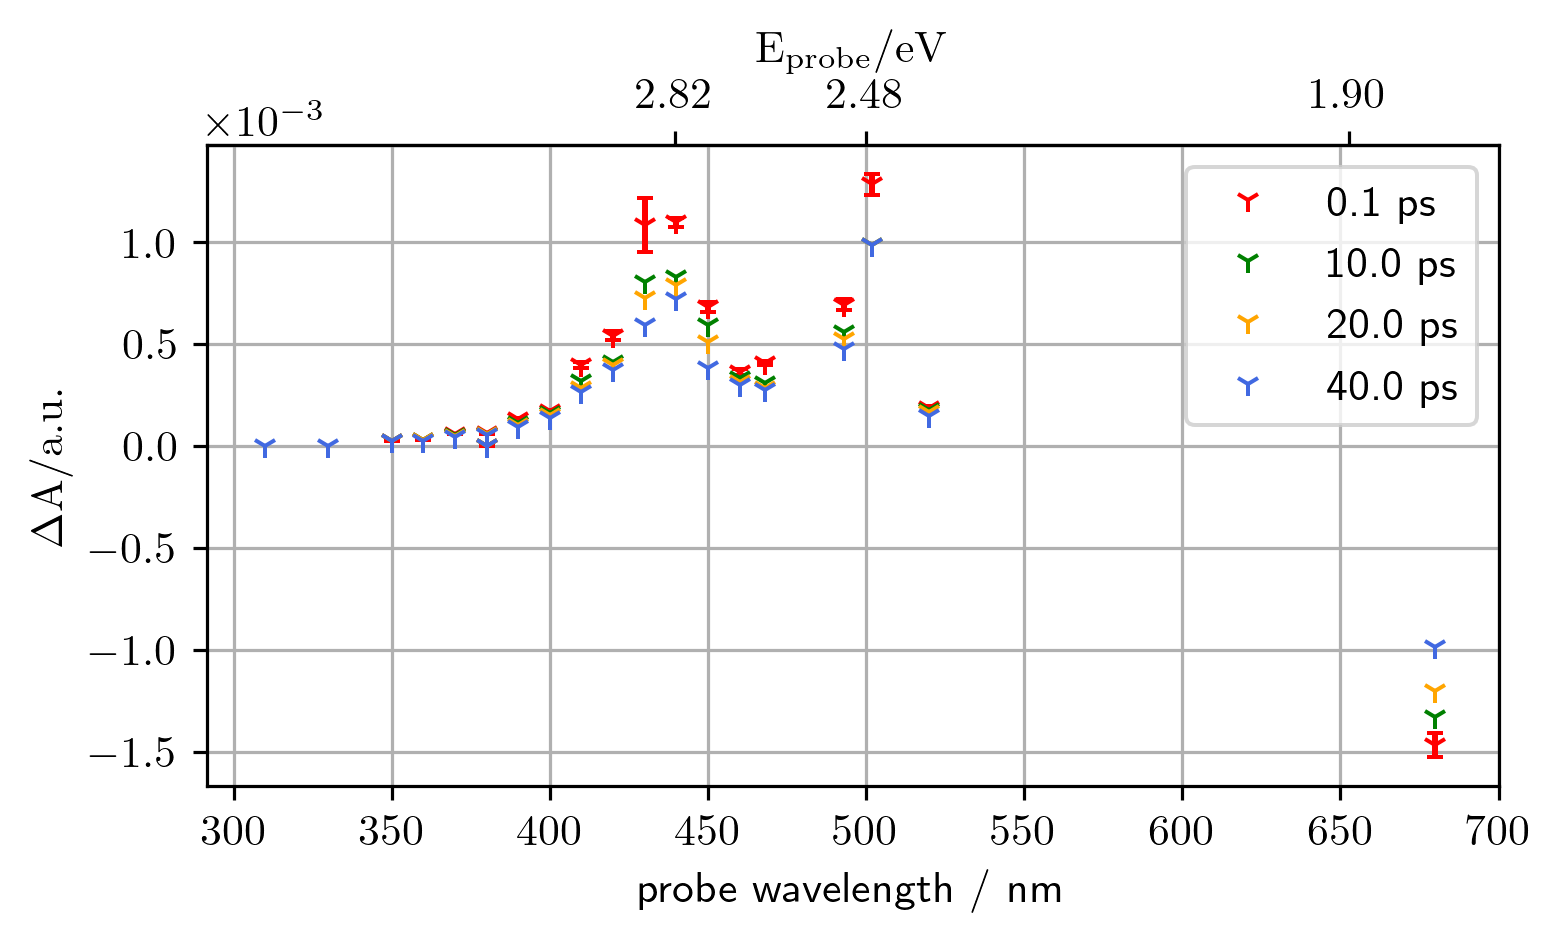
\includegraphics[scale=1]{images/TimeResolvedWavelengthScanSQIB1perc_PMMA_mapCorrected.png}
\caption[Fitted transient absorbance probe spectrum of 1wt\% SQIB PMMA at pump \qty{653}{\nano\meter}.]{Time resolved (fitted) transient absorbance probe spectrum of 1wt\% SQIB PMMA. Errorbars for 0.1 ps based on peak pump radiant exposure uncertainty. Pump wavelength is 653 nm with peak radiant exposures noted in tab. \ref{tab:powersWavScan}. Correction by reference map has been applied. Transient absorbance values calculated from (multi-)exponential decay fits.\label{fig:SQIB_PMMAwavelengthscan}}
\end{figure}

A comparison is made to data for squaraines with n-butyl sidechains by Zheng et al.\cite{Zheng2020} in fig. \ref{fig:TA_vsZheng} and in a zoomed section detailing the ESA bands in fig. \ref{fig:TA_vsZheng}. Notably Zheng\cite{Zheng2020} used a white light probe setup and corrected measurements for anisotropy, leading to a much finer spectrum and slightly different peaks. Due to a moving sample setup Zheng also could use far higher pump power densities, which for our measurement setup would degrade our sample too quickly to acquire a delay scan. Using a white light probe together with a wavelength selective detector leads to a far more precise spectrum compared to the Gaussian spectral distribution probe used here. The measurements are scaled so that the transient absorption immediately after temporal overlap at \SI{680}{\nano\meter} is -1. Reason for that is, in our case the transient behaviour directly on the maximum of the CW absorption band at \SI{653}{\nano\meter} proved hard to correctly measure, which is why an off maximum measurement point was chosen to compare.%madlad used up to 80 nJ/pulse

\begin{figure}[hbtp]
\centering
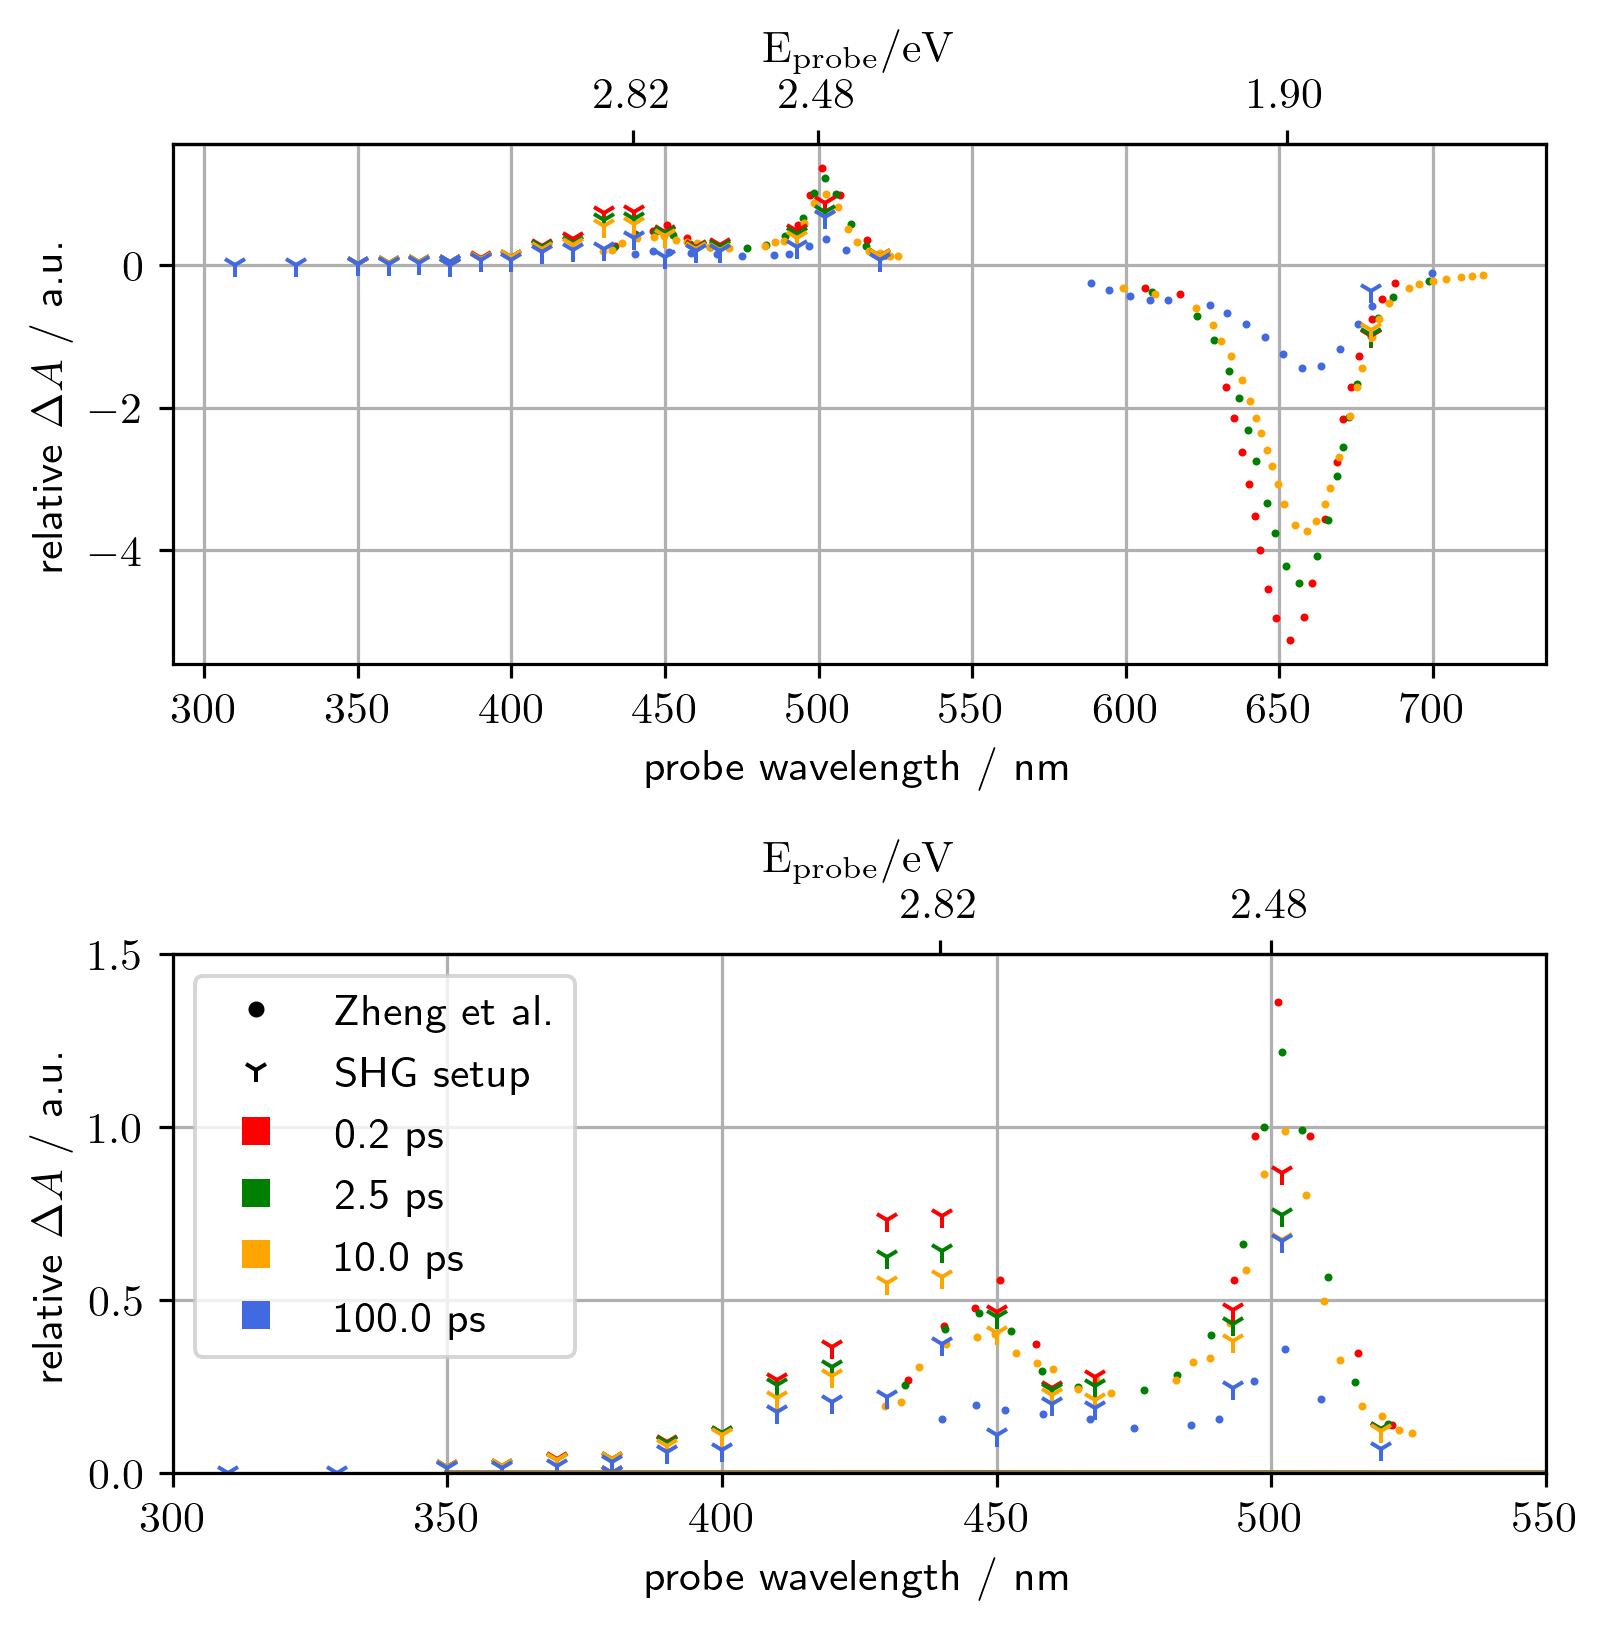
\includegraphics[scale=1]{images/TimeResolvedWavScanvsZheng_Combined.png}
\caption[TA fits of SHG setup 1wt\% SQIB in PMMA compared to Zheng et al.\protect\cite{Zheng2020} squaraine with n-butyl sidechains in PMMA.]{TA fits of SHG setup 1wt\% SQIB in PMMA compared to Zheng et al.\protect\cite{Zheng2020} squaraine with n-butyl sidechains in PMMA.\\ Note the 0.2 ps are below the chosen temporal resolution of our measurement and the 100 ps decay point is purely fit data, as the measurements do not extend past a delay of 50 ps. The ESA section is shown magnified in the lower plot.\\
Zheng measurement is isotropic (considering both parallel and orthogonal pump probe polarization), while the SHG setup measurement is parallel polarization only. Measurements are scaled so that the transient absorption immediately after temporal overlap at \SI{680}{\nano\meter} is -1. Measurements for \SIlist{310;330}{\nano\meter} are from older measurement series, but since no signal was detected are shown as zero here. Zheng data digitised for plotting with WebPlotDigitizer.\cite{Rohatgi2022}\label{fig:TA_vsZheng}}
\end{figure}

%\begin{figure}[hbtp]
%\centering
%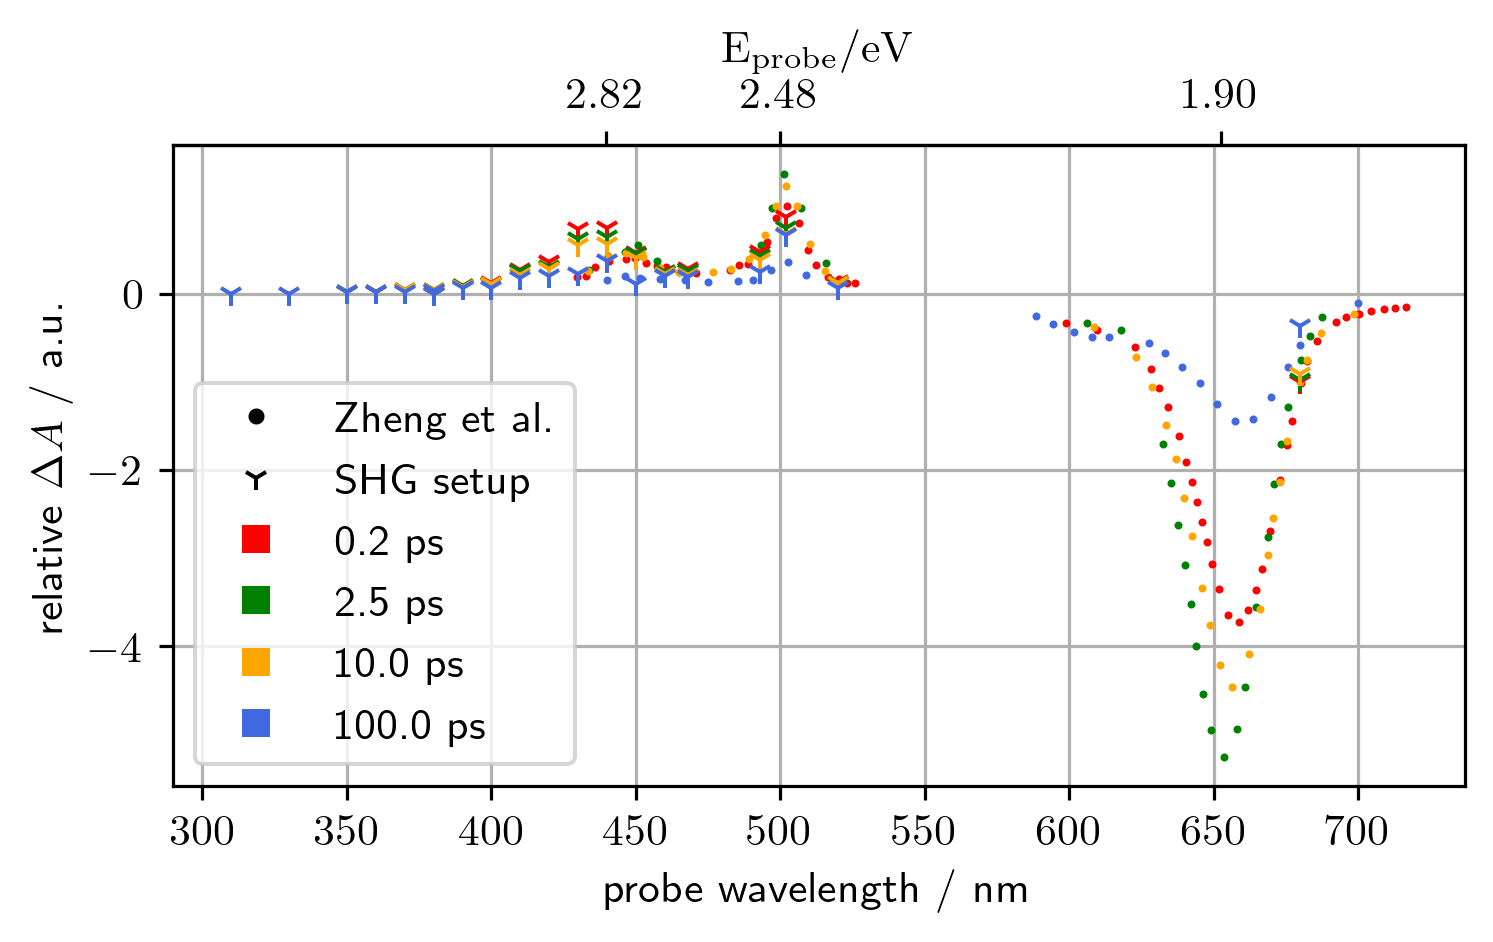
\includegraphics[scale=1]{images/wavScanVsZheng.png}
%\caption{TA fits of SHG setup 1wt\% SQIB in PMMA compared to Zheng et al.\protect\cite{Zheng2020} squaraine with n-butyl sidechains in PMMA.\\ Notably the 0.2 ps are below the chosen temporal resolution of our measurement and the 100 ps decay point is purely fit data, as the measurements do not extend past a delay of 50 ps.\\
%Zheng measurement is isotropic (considering both parallel and orthogonal pump probe polarization), while the SHG setup measurement is parallel polarization only. Measurements are scaled so that the transient absorption immediately after temporal overlap at \SI{680}{\nano\meter} is -1. Measurements for \SIlist{310;330}{\nano\meter} are from older measurement series, but since no signal was detected are shown as zero here. Zheng data digitised for plotting with WebPlotDigitizer.\cite{Rohatgi2022}\label{fig:TA_vsZheng}}
%\end{figure}

%\begin{figure}[hbtp]
%\centering
%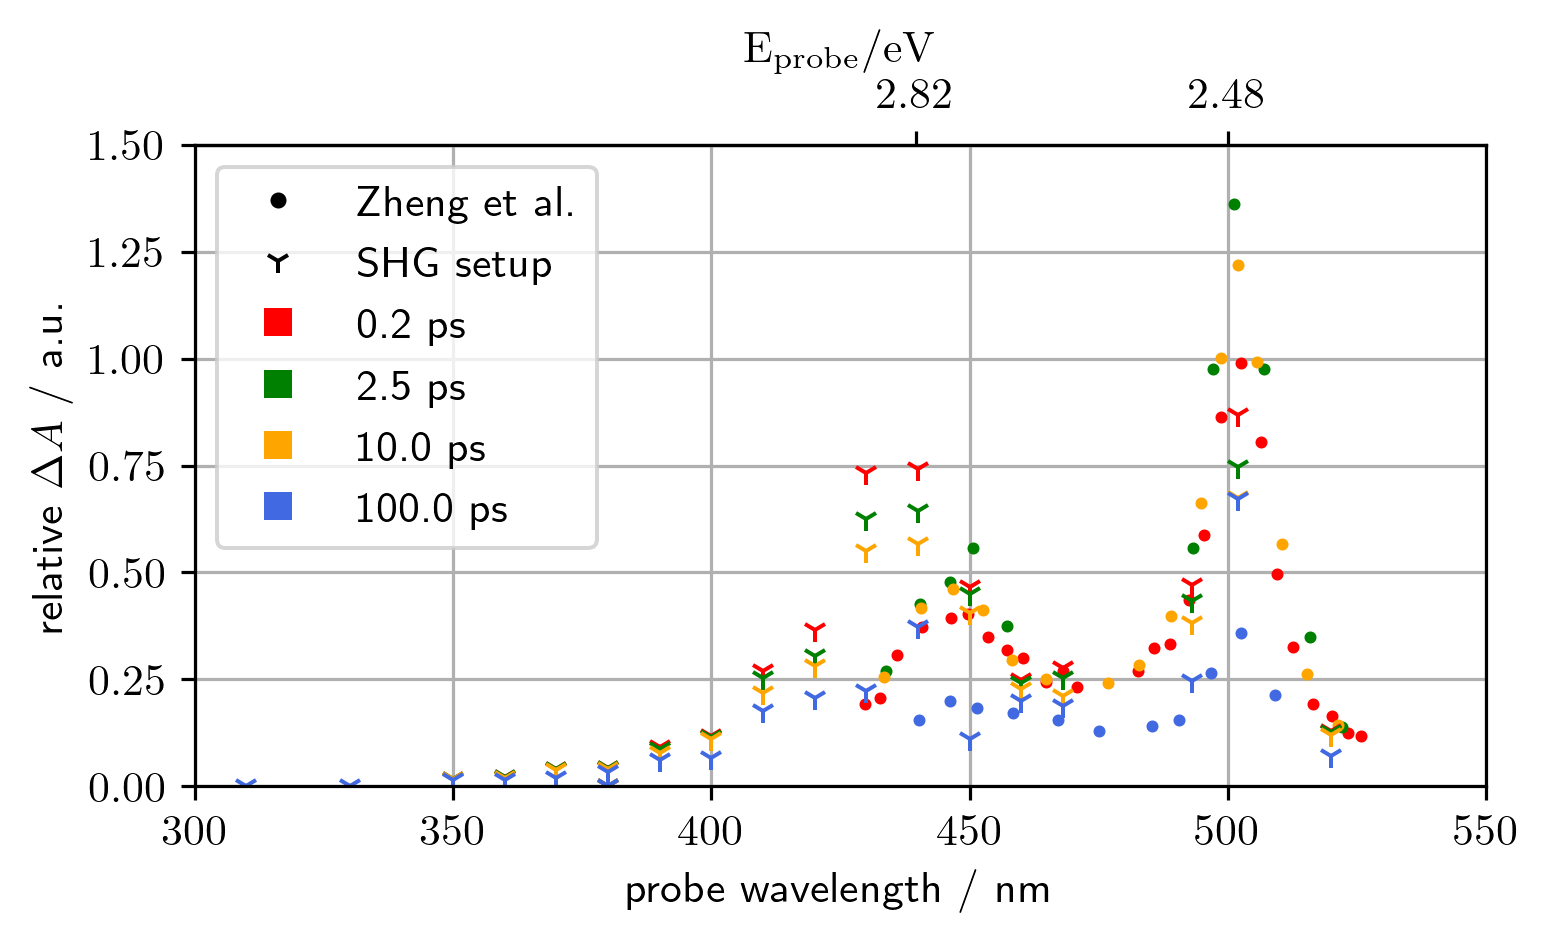
\includegraphics[scale=1]{images/TimeResolvedWavScanvsZheng_Zoom.png}
%\caption{Constricted TA fits of 1wt\% SQIB in PMMA compared to 1wt\% squaraine in PMMA by Zheng et al.\protect\cite{Zheng2020} squaraine with n-butyl sidechains in PMMA.\\ Note the 0.2 ps are below the chosen temporal resolution of our measurement and the 100 ps decay point is purely fit data, as the measurements do not extend past a delay of 50 ps. 
%Zheng measurement is isotropic (anisotropy corrected considering both parallel and orthogonal pump-probe polarization), while SHG-setup is parallel only. Measurements are scaled so that the transient absorption immediately after temporal overlap at \SI{680}{\nano\meter} is -1. Measurements for \SIlist{310;330}{\nano\meter} are from older measurement series, but since no signal was detected are shown as zero here. Zheng data digitised for plotting with WebPlotDigitizer.\cite{Rohatgi2022}\label{fig:TA_vsZheng_Zoomed}}
%\end{figure}


Additionally to the fitted behaviour in fig. \ref{fig:SQIB_PMMAwavelengthscan}, the corrected data is shown "raw" in fig. \ref{fig:SQIB_PMMA_rawWavs}, where the linearly interpolated response is shown relative to the absolute value of the maximum response.
\begin{figure}[htp]
\centering
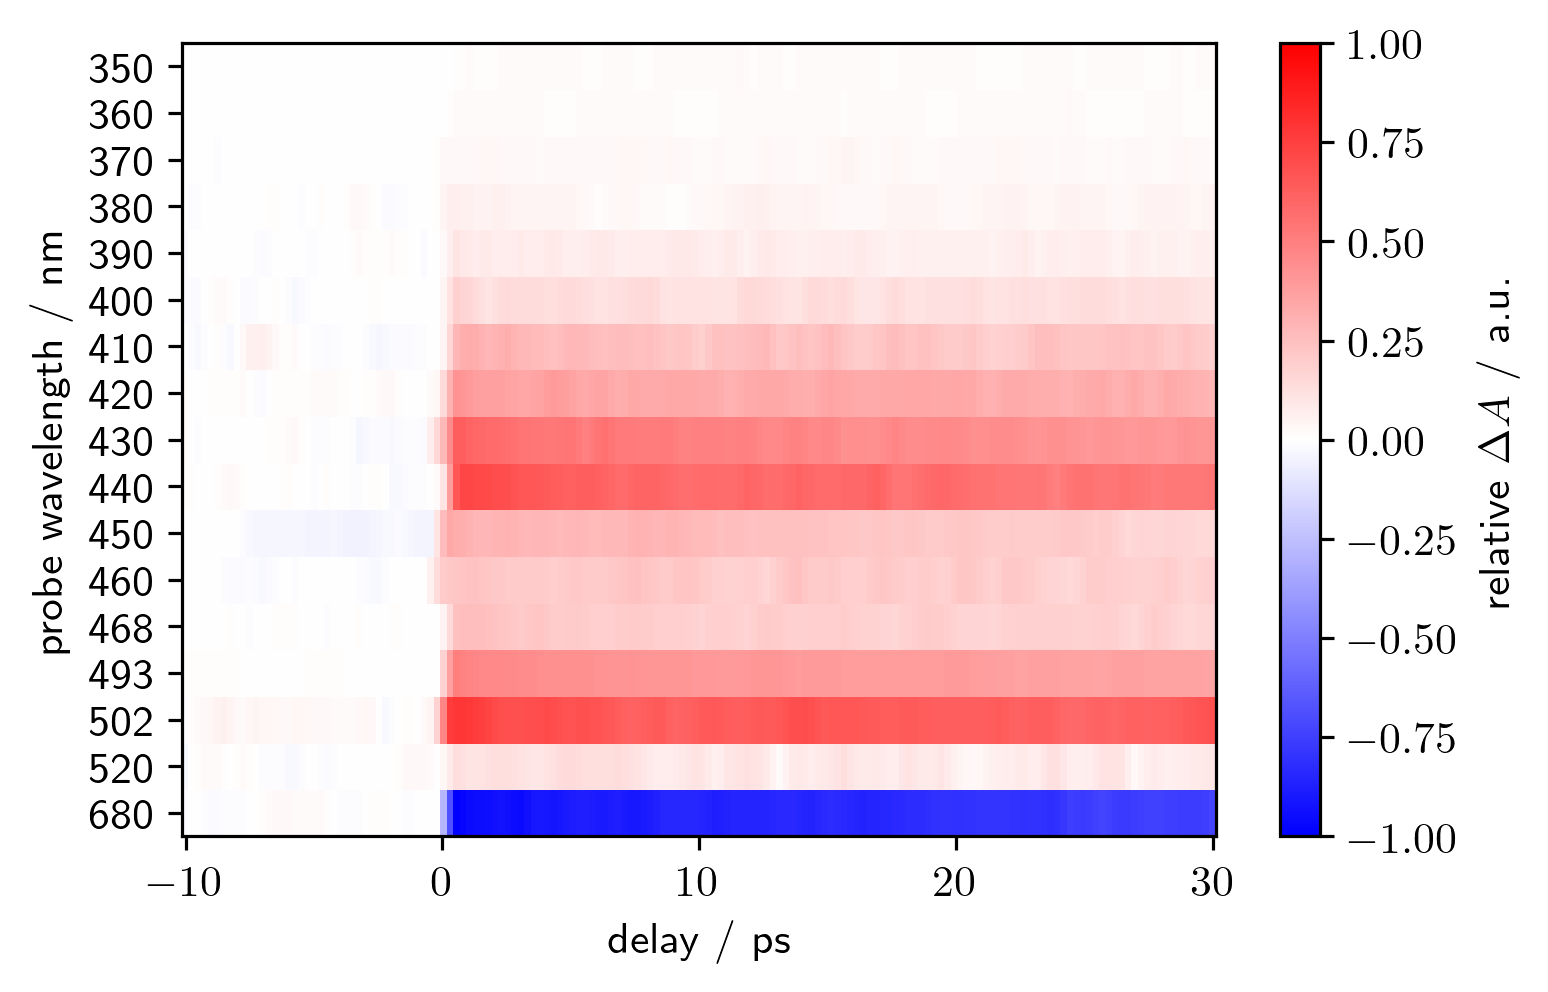
\includegraphics[scale=1]{images/RawishDataWavelengthScanSHG.png}
\caption[Probe wavelength scan at a 653 nm pump wavelength with linear interpolation of time steps.]{Alternative plot of probe wavelength scan at a 653 nm pump wavelength.\\Map correction and degradation correction applied. The data shown is a linear interpolation of the datapoints using numpy.interp(). Delay scans are aligned to their fitted pump probe temporal overlap delay. Ordinate shows centroid probe wavelengths.\label{fig:SQIB_PMMA_rawWavs}}
\end{figure}
\paragraph{Pump and probe wavelengths}
Note again that the pump and probe pulses are not monochromatic but have an extended chromatic spectrum. Pump FWHM is expected to be in the range of \SI{23}{\nano\meter} with the centroid being \SI{653}{\nano\meter} as shown in fig. \ref{fig:specRefPump}. For the probe pulse things are slightly more complicated, where the output directly from the NOPA is straight forward and the centroid is set to the noted value. For SHG on the other hand, the spectrum ahead of the cage is usually not measured, thus the wavelength noted is half the wavelength of the fundamental centroid. Keeping the fundamental intensity near the SHG threshold restricts the possible phase matching wavelength shift. At most a shift to the half values of the spectral distribution may be expected at high irradiances and less for irradiances near the threshold of SHG. Examples for probe spectra similar to the ones used in measurements are shown in fig. \ref{fig:probeSpectra}.
\paragraph{PMMA background}
A quick TA measurement for a PMMA only sample was done for a 653 nm pump with probe wavelengths of \SI{370}{\nano\meter} and \SI{440}{\nano\meter},  wavelengths where PMMA is highly transmitting, and at reasonable pump powers no signal response was detected. Pushing it to unreasonable pump powers at the edge of white light generation there may be slight ESA, however at these powers the measurement technique is fundamentally flawed due to excessive stray light. This rules out the long shoulder of the higher energy ESA peak being an effect of purely the PMMA used for the solid solution.




\chapter{Examination of Reliability}\label{chpt:reliability}
Some tests have been done to ascertain the validity and stability of the corrections devised for the UV extended TAM. The same 1wt\% SQIB in PMMA sample is used for following measurements.
\section{Sample irregularities}
As mentioned above, irregularities over the area of the sample probed were attempted to linearly compensate for with a reference map, at a pump 653 nm probe 680 nm combination. The attempt of a linear compensation does make sense if the variation is of sample thickness, but not necessarily for density variations, see sec. \ref{deriv:RadianceResponse}. In case of drastic density variation, features that are not of the plain coulombic monomer spectrum could be amplified and the states measured be quenched more quickly than for the monomer. Comparing the 1wt\% and 4wt\% graphs of the CW absorption spectra, it seems likely that even a sample density variation of $\pm100\%$ would not lead to a response differing from the monomer response at the sample position.

\section{Power density dependence}\label{sec:powerVar}
For measurements to be valid there should be a linear correspondence of pump irradiance and the measured transient absorbance. Main concern here is that pump irradiance is within the linear regime of the transient absorption response. For the probe pulse the linear response of the sample is also important. In case of a too high irradiance the sample may saturate as well, which can influence the response in two ways additional to processes involving more than one photon: First, for a probe wavelength experiencing ESA, assuming no absorption in the groundstate, the ESA response would be reduced, just like population transfer from the groundstate leads to GSD, see fig. \ref{fig:photonSatESA}. Secondly, for a GSD probe wavelength it would lead to further reduction in absorption and an increase of the response, see fig. \ref{fig:photonSatGSD}.\\

\begin{figure}[h]
\centering
\begin{subfigure}[b]{0.5\linewidth}
\centering
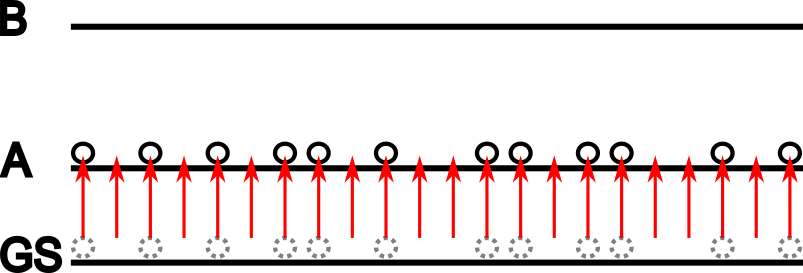
\includegraphics[scale=1]{images/TA_saturation_GSD.png}
\caption{Photon saturation for GSD. Similarly for pumping the sample the linearity in irradiance for sample response is no longer given.\label{fig:photonSatGSD}}
\end{subfigure}\hfill
\begin{subfigure}[b]{0.5\linewidth}
\centering
\includegraphics[scale=1]{images/TA_saturation_ESA.png}
\caption{Photon saturation of ESA active sample leads to reduction of measured sample response or may even show as GSD.\label{fig:photonSatESA}}
\end{subfigure}
\caption[Visualisation of photon saturation behaviour for GSD and ESA.]{Irradiance saturation of sample leads to an increase in transmission and may add or subtract from sample response if photon density is too high. Nearly all possible excitations are excited, with many excess photons passing the sample unperturbed.  GS is the ground state and A, B are states with allowed transitions.}
\end{figure}

To test this multiple pump and probe power combinations were tested at the same sample position. Only variable linear neutral density filter insertion was changed to change the attenuation. Insertion depth of the variable ND filters was assumed to not change the overlap and only the starting overlap was recorded. This was not done at the same calibration as the wavelength scan; however, since no change to pump or probe positions were made this should be a general reference to the behaviour, that does not depend as much on perfect pump probe overlap. The linearity of the sample is shown for radiant exposures up to $\radiantExp=$\pumpExp{295e-3} \SI{653}{\nano\meter} pump and $\radiantExp=$\probeExp{91e-3} \SI{680}{\nano\meter} probe combinations. Note that these points were measured at the same sample spot, thus sample degradation is a factor to consider. Specifically the graph showing the probe irradiance dependence in fig. \ref{fig:powerVarCorrection} shows sample degradation due to the high pump power density. Notably the higher power density measurements agree far better regarding degradation correction. There is no obvious reason for the low probe irradiance measurement, corresponding to the first measurement of the three, having a slightly stronger response. The second measurement at a probe radiant exposure of $\radiantExp=$\probeExp{90e-3} responds very well to the applied degradation correction and all three sub-measurements coincide. This implies that the decreased response is not just based on faster degradation due to probe influence.

\begin{figure}[p]
\begin{subfigure}[t]{0.5\linewidth}
\centering
\includegraphics[width=\linewidth]{images/PowerVariationCorrectedPump.png}
\caption{Influence of variation of pump radiance on signal. Data points at the lowest $\radiantExp$ are three measurements with varied probe radiant exposures in range of $\radiantExp=\SIrange{114e-4}{458e-4}{\radExp}\frep{40}$, with raw data shown in fig. \ref{fig:PowerVarL}. They show a minimal spread in response.}
\end{subfigure}\hfill
\begin{subfigure}[t]{0.5\linewidth}
\centering
\includegraphics[width=\linewidth]{images/PowerVariationCorrectedProbe.png}
\caption{Influence of variation of probe radiance on signal at pump radiance $\radiantExp=\SI{218e-3}{\radExp}\frep{20}$. Measurements were made in order left, right and center.\label{fig:PowerVarProbe}}
\end{subfigure}
\caption[Influence of variation of radiant exposures on signal for pump \SI{653}{\nano\meter} and probe \SI{680}{\nano\meter}.]{Influence of variation of radiant exposures on signal for pump \SI{653}{\nano\meter} and probe \SI{680}{\nano\meter}. Uncertainties based on radiant exposures $\radiantExp$.
Overlap corrected data in \textcolor{blue}{blue} and additionally pump degradation corrected data in \textcolor{red}{red}. Every point shown is the average of a triple delay scan measurement fitted with a single exponential decay.\\ The relatively high probe intensity in the GSD band of squaraines may be the reason for an error in degradation compensation in fig. \ref{fig:PowerVarProbe}, since the highest probe radiance is the second measurement point. \label{fig:PowerVarRaw}}
\end{figure}

\begin{figure}[hp]
\centering
\begin{subfigure}[t]{0.45\textwidth}
\centering
\includegraphics[scale=1]{images/PowerVarLowPumpVarProbe.png} 
\caption{Pump radiant exposure $\radiantExp=$\pumpExp{31e-3}\\TA\_fourier measurements:\\ 6615-6620, 6630-6632\label{fig:PowerVarL}}
\end{subfigure}
\hfill
\begin{subfigure}[t]{0.45\textwidth}
\centering
\includegraphics[scale=1]{images/PowerVarHighPumpVariedProbe.png} 
\caption{Pump radiant exposure $\radiantExp=$\pumpExp{221e-3}\\TA\_fourier measurements:\\ 6645-6653\label{fig:PowerVarR}}
\end{subfigure}
\caption[Raw transient absorption delay scans of pump \qty{653}{\nano\meter} with varied probe \qty{680}{\nano\meter} radiant exposure.]{Raw transient absorption delay scans of pump \qty{653}{\nano\meter} with varied probe \qty{680}{\nano\meter} radiant exposure.
For both sub-plots the probe power density is varied. The influence on the decay of signal response on the right subplot is due to high powers inducing stronger degradation in the sample.}
\end{figure}

\section{Overlap correction value accuracy}
As laid out in section \ref{sec:CorrFactor} a correction factor is calculated for every measurement point to compensate overlap error in lateral position, as well as in relative size of pump and probe beam.
To check this, measurements with varying overlap were taken, for which the fits can be seen in fig. \ref{fig:correctionComparison}.\\
Pump and probe point spread functions are measured together for every measurement, but the pump beam is not altered in any way. The corrected output is shown in tab. \ref{tab:ArtCorrTest}.\\

\begin{figure}[H]
\centering
\includegraphics[width=\linewidth]{images/CompensationTestFitted.png}
\caption[Beam fits for overlap correction testing plotted along with their overlap correction.]{Beam fits plotted along with their overlap correction. Raw beam shapes are shown compared to fits in fig. \ref{fig:rawVsFittedBeam}.\label{fig:correctionComparison}}
\end{figure}

A comparison between the correction factors acquired through the fits, as shown in fig. \ref{fig:correctionComparison}, and the numeric correction factor from ArtFit.getNumericCorrection, using an interpolation point density setting of 32 points per $\sigma$, is shown in tab. \ref{tab:numVsfittedCorrection}. They are relatively similar as expected from the results in figures \ref{fig:NumericalCorrectionSNR} and \ref{fig:NumericalCorrectionShift}, when considering the pixel density of the camera against the dimension of the point spread functions. For badly fitted point spread functions the numeric variant with interpolation is likely the better choice, but for well shaped beams the analytic fitted correction values should be preferred for the current setup.



\begin{table}[H]
\caption[Overlap corrected transient absorption values from fitted bi-exponential decay at time 0.]{Overlap corrected transient absorption values from fitted bi-exponential decay at time 0. Uncertainty only includes overlap and pump radiant exposure and ignores delay scan fitting uncertainty. Beam pairs shown in fig. \ref{fig:correctionComparison}.\label{tab:ArtCorrTest}}
\centering
\begin{tabular}{cllllr}\toprule
\multirow{2}{*}{beam pair} &\multicolumn{2}{c}{x} & \multicolumn{2}{c}{y} & \multirow{2}{*}{$\Delta A$ / $\si{\od\joule\per\square\meter}\cdot \qty{20}{\kilo\hertz}$} \\
&$\sigma_1/\sigma_2$ / px & $\mathrm{\Delta}\mu$ / px & $\mathrm{\Delta}\mu$ / px & $\mathrm{\Delta}\mu$ / px &  \\ \midrule
a)&$0.85 \pm 0.02$           & $0.46 \pm 0.05$            & $0.71 \pm 0.01$            & $0.25 \pm 0.02$            & \qty{7.6(5.0)e-4}{}                        \\
b)&$0.87 \pm 0.02$           & $3.11 \pm 0.05$            & $0.74 \pm 0.01$            & $0.15 \pm 0.02$            & \qty{4.7(3.3)e-4}{}                        \\
c)&$1.57 \pm 0.04$           & $0.19 \pm 0.06$            & $1.21 \pm 0.02$            & $0.12 \pm 0.04$            & \qty{6.5(4.8)e-4}{}                        \\
d)&$0.71 \pm 0.02$           & $0.03 \pm 0.05$            & $0.58 \pm 0.01$            & $0.02 \pm 0.02$            & \qty{7.2(5.4)e-4}{} \\\bottomrule                      
\end{tabular}
\end{table}


\begin{table}[H]
\caption[Overlap correction for beam pairs shown in fig. \ref{fig:correctionComparison}.]{Overlap correction for beam pairs shown in fig. \ref{fig:correctionComparison}. Beam pair parameters are shown in tab. \ref{tab:ArtCorrTest}. The fitted correction values are the product of the individually calculated x and y correction factors.\label{tab:numVsfittedCorrection}}
\centering
\begin{tabular}{ccrrrr}
\toprule
\multicolumn{2}{c}{beam pair} & a) & b) & c) & d) \\ 
\midrule
\multirow{3}{*}{fitted correction} & x & 1.329& 2.449& 1.864& 1.229\\
& y & 1.230& 1.243& 1.573& 1.155\\
& total & 1.635 & 3.044 & 2.933 & 1.419 \\ \midrule
\multicolumn{2}{c}{numeric correction} & 1.656 & 2.936 & 3.025 & 1.421 \\ 
\bottomrule
\end{tabular} 
\end{table}





\section{Sample degradation}\label{sec:degradation}
The main loss of sample response is suspected to be dependent on the pump pulse, as it is right at the CW absorption peak. A repeated delay scan at the same position is shown in fig. \ref{fig:rawDegradation}, to show degradation behaviour. That combined with the higher peak irradiance of the pump pulse makes it the prime candidate of photo bleaching. This would also be supported by the circumstance, that a pump probe wavelength combination fully on the main absorption peak always showed a lower GSD response than expected. Reasoning for that may be fast degradation of the sample spot where pump and probe coincide in their peak irradiances. Higher irradiances were used at that point, making this even more likely.\\
The pump pulse on the main absorption peak is expected to be the main degrading component, for most of the probe spectrum, as long as low probe peak irradiances are used. For high probe photon energies this may no longer be the case, however from the spectra recorded so far no indication of a strong influence is seen for the sample used.\\
Reduction of transient response at a pump peak irradiance of \qty{653}{\nano\meter} at $\radiantExp\,=\;$\pumpExp{79(4)e-3} combined with a probe wavelength of 493 nm at $\radiantExp\,=\;$\probeExp{8.6(1.3)e-3}, which is close to the main absorption peak of the lower energy ESA transition of the monomer, is tested here. The time dependence is taken as a series of typical measurements. This mainly serves to confirm the typical measurement behaviour and to make an attempt at correcting for the response loss due to photo bleaching.

\begin{figure}[hbtp]
\centering
\includegraphics[width=\linewidth]{images/DegradationRAWPump653Probe493.png}
\caption[Raw data from degradation series of identical measurements at same spot at pump \SI{653}{\nano\meter} and probe \SI{493}{\nano\meter}.]{Raw data from degradation series of identical measurements at same spot at pump \SI{653}{\nano\meter} \pumpExp{79(4)e-3} and probe \SI{493}{\nano\meter} \probeExp{8.9(1.3)e-3}.
Time at start on the y axis corresponds to the starting time of the measurement\label{fig:rawDegradation}}
\end{figure}
Usually photobleaching is modelled by an exponential decay as a function of exposure time. A fit is made to the decay of the absorbance $\frac{\Delta A\left(t\right)}{\Delta A\left(t=0\right)} = \mathrm{exp}\left(-\frac{t}{\tau}\cdot f_{rep}\cdot\radiantExp\right)$.
All datapoints after the temporal overlap, which are background subtracted, are used in fitting. This avoids strong variations in the pre-temporal-overlap area, where the absorbance values vary mildly around 0 mOD leading to a strong variation of their ratio and an ill-conditioned fit. A nonlinear least squares approach with scipy curve\_fit is used to minimize a residual defined as
\begin{equation}\label{eq:degradationFitting}
\mathrm{residual} = \sum_{t_{\text{start},i},d_j} \left(ln\left(\lvert\frac{\Delta A(t_{\text{start},i},d_j)}{\Delta A(t=0,d_j)}\rvert\right)- \frac{t_i}{\tau}\right)^2
\end{equation}
Here $t_i$ is the time at the start of the scan, $d_j$ is the delay between pump and probe pulses and $\tau$ is the decay parameter fitted. The absolute value of change in absorbance is taken to avoid negative values in the logarithm, even though they are unlikely when only $d_i$ after temporal overlap are used.  This simplification is needed, as only starting times of delay scans are collected. A moving mean may be used to smooth particularly noisy data. Used fits use a moving mean of 5 measurement points. Compared to no smoothing mean, it does not change the fit result in a significant way, though the data here is not particularly noisy.\\
The correction applied to the delay scans assumes an equal time for each measurement point based on the mean time between two delay scans and the number of points in the scan. The equation equivalent to the compensation is shown in eq. \ref{eq:degradationCompensation}. In fig. \ref{fig:degradationCorrectionComparison} a comparison of raw and corrected data is shown. The decay corrected data shows a far lower spread in absorbance values making the fitting method a valid option. 

\begin{equation}\label{eq:degradationCompensation}
\Delta A_\text{compensated}(t_i(d_j), d_j) = \delta A(t_i(d_j), d_i)\cdot \mathrm{exp}\left(+\frac{t_i(d_j)-t0}{\tau_{1/e}}\right)
\end{equation}

\begin{equation*}
t_i(d_j) = t_i + j\cdot \mathrm{mean}(\Delta t_\mathrm{delay\, scan)}
\end{equation*}

\begin{figure}[hbtp]
\centering
\begin{subfigure}[t]{0.4\linewidth}
\centering
\includegraphics[scale=1]{images/DegradationRAWPump653Probe493-Graph.png}
\caption{Raw data as in fig. \ref{fig:rawDegradation}}
\end{subfigure}
\hfill
\begin{subfigure}[t]{0.4\linewidth}
\centering
\includegraphics[scale=1]{images/DegradationCorrectedPump653Probe493-Graph.png}
\caption{Exponential decay corrected data\\
Decay constant $\tau_{1/e}$ = \SI{12600}{\second} at $\radiantExp\,=\;$\pumpExp{79(4)e-3}}
\end{subfigure}
\caption{Comparison of raw data and decay corrected data for measurements TA\_fourier: \mbox{6778 - 6787}.\label{fig:degradationCorrectionComparison}}
\end{figure}



\begin{figure}[hbtp]
\centering
\begin{subfigure}[t]{0.3215\linewidth}
\centering
\includegraphics[width=\columnwidth]{images/PowerVarHigh_Raw.png}
\caption{Raw data as in fig. \ref{fig:PowerVarR}}
\end{subfigure}
\hfill
\begin{subfigure}[t]{0.3215\linewidth}
\centering
\includegraphics[width=\columnwidth]{images/PowerVarHigh_CorrNative9900.png} 
\caption{Corrected per native fit at $\tau_{1/e}=$\SI{9900}{\second}}
\end{subfigure}
\hfill
\begin{subfigure}[t]{0.3215\linewidth}
\centering
\includegraphics[width=\columnwidth]{images/PowerVarHigh_CorrEstimate12600_2.8.png} 
\caption{Corrected from degradation fit fig. \ref{fig:degradationCorrectionComparison}\\
$\tau_{1/e}=$\SI{14100}{\second}, $H_{ratio}=\frac{H_\text{\SI{680}{\nano\meter}}}{H_\text{reference:\SI{497}{\nano\meter}}} = \frac{218}{79}= 2.8$}
\end{subfigure}
\caption[Comparison of pump \SI{653}{\nano\meter} probe \SI{680}{\nano\meter} raw data, degradation corrected by directly fitted and adapted, power corrected, decay constant.]{Comparison of pump \SI{653}{\nano\meter} probe \SI{680}{\nano\meter} raw data, corrected by direct fit and by applying the decay constant gathered from fig. \ref{fig:degradationCorrectionComparison}. Using the power correction as a ratio factor of used measurement \radiantExp divided by fitting \radiantExp as follows $\Delta A(t) = \Delta A(t=0)\cdot \mathrm{e}^{-\frac{t\cdot H_{ratio}}{\tau}}$, where $\frac{H_\mathrm{measurement}}{H_\mathrm{reference}} =1$, if the \radiantExp is the same as for the measurement where degradation is fitted, and t is the elapsed times since start of the measurement. Note that the measurements gathered in this figure have different probe power densities.\label{fig:powerVarCorrection}}
\end{figure}
\paragraph{Probe wavelengths}
Note that the probe wavelengths compared here may correspond to different processes within the molecules. The degradation of the first ESA transition corresponds to an effect of inactivation of the excited state reachable from the pumped state or to a reduction of molecules which can be pumped. The GSD measurement instead directly measures the reduction in squaraine absorption, with the probe wavelength likely just adding to the pump irradiance for degradation with a weighting factor of the different absorption cross-section for its wavelength. If degradation times coincide for GSD and ESA, then the likelihood of having a shared degradation pathway is relatively high. Additionally, the probe wavelength may also introduce another degradation pathway or mediate a faster degradation via the same pathway as the GSD pathway. The single exponential degradation is only justified by it seemingly providing a decent output, as well as the use case and measurement data not warranting better modelling. A description of different pathways for organic fluorophores may be found, including their behaviours; however, they strongly vary for different molecules making them unpredictable for untested molecules.\cite{Demchenko_2020}

\paragraph{Power dependence}
A simple naive assumption for power dependence of photobleaching is equal bleaching for equal total dose. This ignores photobleaching pathways and power density dependencies. It is unknown if this is truly applicable for the used peak powers, since references for other fluorophores usually used CW methods, while pulsed operation with similarly high peak powers may very well behave differently. Since the actual power dependence here is beyond the scope of the thesis, the naive assumption is attempted. Here the dependence of photo degradation is a direct product of the power density on the exposure time, for total dose the sample is exposed to, $e^{-\frac{t\cdot \radiantExp\cdot f_{rep}}{\tau}}$, where $t$ is the exposure time and $\radiantExp$ is the peak radiant exposure per pulse and $f_{rep}$ is the repetition rate of the pump pulse.\cite{Eggeling1998}
A comparison of the degradation in the measurements in fig. \ref{fig:degradationCorrectionComparison} with a probe wavelength of \SI{497}{\nano\meter} and fig. \ref{fig:powerVarCorrection} is made, to show the decreased spread of the corrected data.

Another aspect to consider is the power density influence on degradation, for which the measurements from sec. \ref{sec:powerVar} are used.  Their decay constant shows $\tau_{1/e}\left(\SI{218e-3}{\radExp}\right)=\SI{9900}{\second}$  opposed to the $\tau_{1/e}\left(\SI{79e-3}{\radExp}\right)=\SI{12600}{\second}$. The fit from the degradation series, when corrected for total dose rate, seems to fit better with all measurements close together, while the fit made on the power variation measurements leads to a lot wider spread. The effect of the constants on the measurements is shown in fig. \ref{fig:powerVarCorrection}.

A not so naive model for degradation would need to account for the beam shape and overlap of pump and probe beams, as this would change sensitivity according to the pump intensity profile, which in turn would increase relative response near the FWHM of the pump beam profile. The high power density area on the sample, however, would also decay quicker, because photodamage tends to be at least linearly dependent on the total dose. The naive model seems sufficient for this measurement resolution at good overlap.

\section{Polarisation}
Only having the parallel polarisation recorded is unfortunate, however for pump \SI{653}{\nano\meter} probe \SI{440}{\nano\meter} an orthogonal measurement exists. The measurement is shown in fig. \ref{fig:polarisationComp}, where a moving mean is used to smooth data slightly. The parallel measurement is roughly two times the orthogonal measurement at temporal overlap. For an isotropy corrected measurement, see section \ref{sec:PolAngles}, that would mean that the corrected measurement would be nearly the same. The anisotropy r at zero time however shows a deviation from the expected value of r = 0.4, which would be expected for parallel pump and probe transition dipole moments. A measurement error for the orthogonal measurement cannot be ruled out. Using the Perrin formula $\mathrm{r} = \frac{1}{5}(3\mathrm{cos}^2\beta-1)$ a hypothetical angle of $\beta \approx \ang{30}$ between pump and probe transition dipole moments is calculated. No sensible insight for a physical reason may currently be given for this. 


\begin{figure}[hbt]
\centering
\begin{subfigure}[t]{0.49\linewidth}
\includegraphics[scale=1]{images/440nm_ParallelOrthComparison.png}
\caption{Orthogonal and parallel TA measurements, degradation and sample variation corrected. Orthogonal values multiplied with 2.\label{fig:polarisationComp}}
\end{subfigure}
\hfill
\begin{subfigure}[t]{0.49\linewidth}
\includegraphics[scale=1]{images/440nm_ParallelOrthComparison_anisotropy.png}
\caption{Anisotropy plotted according to $r = \frac{I_\parallel-I_\perp}{I_\parallel + 2 I_\perp}$.}
\end{subfigure}
\caption[Moving mean transient absorption scan comparison and anisotropy development for orthogonal and parallel pump \qty{653}{\nano\meter} and probe \qty{440}{\nano\meter}.]{Moving mean, temporal overlap aligned, parallel and orthogonal polarisation TA measurements for pump 653 nm probe 440 nm. Moving mean as bins of \SI{2}{\pico\second} size. Bin of value \qty{0}{\pico\second} is aligned with temporal overlap data.\label{fig:440nmPolarisations}}
\end{figure}

\chapter{Outlook}
\section{Experimental setup}
The current experimental setup should be reliable enough for UV probe measurements, however with how laborious acquiring these measurements is it is preferred to use the objectives instead of the lenses if wavelengths with larger wavelengths than \qty{400}{\nano\meter} or energies lower than \qty{3.1}{\electronvolt} are used. The existing setup should have improvised components, such as SHG focus travel stage, replaced when appropriate and if needed.\\
A next step for the setup is the planned inclusion of a wavelength dispersive detector along a white light generation stage. This will allow a vastly improved measurement speed for non-UV wavelengths, along with an even better time resolution, with wider chromatic range improving the transform limited pulse length.

\section{Squaraines}
With the now UV extended transient absorption capability of the setup new theoretical simulations may be confirmed and improved upon. Further simulations, beyond the capability for the essential states model of Robert Schwarzl in the Koch Group, are now contributed by the Puschnig Group at Karl Franzens University Graz.\\
Measurements of samples with an external Institution are planned to be done within the next year, which are meant to confirm both the transient behaviour of our samples as well as shine a new light onto squaraines and their transient behaviour with ellipsometry techniques.


\setcounter{chapter}{0}
\renewcommand\thechapter{\Alph{chapter}}


\chapter{List of Devices}
\let\cleardoublepage\clearpage
\begin{longtable}{p{0.48\textwidth}p{0.48\textwidth}}
    \caption{List of devices used}
    \label{tab:devices} \\
    \toprule 
    Title & Remarks \\
    \midrule
    \endfirsthead
    \toprule 
    Title & Remarks \\
    \midrule
    \endhead
    \midrule
    Continued on next page
    \endfoot
    \bottomrule
    \endlastfoot
    Light Conversion PHAROS & Yb:KGW femtosecond laser, PH1-20-0400-02-30, L191103; \SI{40}{\kilo\hertz} repetition rate at \SI{400}{\micro\joule} pulse energy \\
    Light Conversion ORPHEUS N-3H & NOPA, $ \lambda = \SIrange{500}{950}{\nano\meter} $ \\
    Light Conversion ORPHEUS N-2H & NOPA, $ \lambda = \SIrange{640}{950}{\nano\meter} $ \\
    Scitec 310 CD with 300CD200HS & Optical chopper, frequency $\approx \SIrange{1000}{55000}{\hertz}$, focusing on chopper wheel using two $f=\SI{125}{\milli\meter}$ plano-convex N-BK7 lenses \\
    Scitec S310Sync synchroniser & Phase and frequency locking of the chopper to external sources (function generator, laser sync output, frequency divider) \\
    Thorlabs AHWP05M-600 & \SIrange{400}{800}{\nano\meter} achromatic $\frac{\lambda}{2}$ plate \\
    Thorlabs AHWP10M-980 & \SIrange{690}{1200}{\nano\meter} achromatic $\frac{\lambda}{2}$ plate \\
    Thorlabs NExxA series, Thorlabs NDxxA series, Eksma Optics 240-25xx series & Reflective and absorptive neutral density filters, used for coarse power setting \\
    Reflective variable neutral density filters
NDL-25C-2 & Used to set input power exactly \\
    SCHOTT BG39, UG5  & Spectral glass filters.\\
    Thorlabs FESH0700 & Sputtered short-pass filters \\
    Thorlabs FELH0700 & Sputtered long-pass filter \\
    Thorlabs WP25M-UB & Ultra-broad wire grid polariser \\
    Olympus UPlan FL N 10x & Focussing objective, 10x magnification, NA=0.3 \\
    Nikon Plan 10/0.3 160/0.17 & Imaging objective, 10x magnification, NA=0.3 \\
    EKSMA 110-1216ET& plano-convex UVFS lenses\\
    EKSMA 110-1209ET& UVFS lens for SHG stage\\
    mounted prism & UV translucent, unknown model\\
    Linos HighLED White & For visible imaging microscopy \\
    Sample illumination LED ring & 658 nm (measured), LT3080 current regulation for 12 V input \\
    The Imaging Source DMK 42AUC03 & Monochrome camera, particularly for spatial overlap alignment, beam shape characterization and orientation on the sample \\
    Artray ARTCAM-092UV-WOM & UV sensitive CMOS camera, used for spatial overlap\\
    Detector A & See previous work by Schwarzl \cite{Schwarzl2022} \\
    Picoscope 5442D & Oscilloscope used for data collection from optical detectors \\
    Coherent LabMax Pro & Pulse measuring head, used for optimizing OPA output \\
    Coherent FieldMate with OP2-VIS measuring head & Laser power meter, used for setting input power, partially damaged leading to higher low intensity readings (SN: 1019L08R) \\
    Newport LTA-HS & Delay stage actuator \\
    Thorlabs Z825B, KDC101 & Microscopy sample stage actuators (horizontal and vertical) \\
    Various aluminium mirrors & Protected UV enhanced \\
    74HC73 & Dual JK flip-flop for frequency division\\
    Ocean Optics Flame-S & Grating spectrometer with optical fiber and diffusor. SN: FLMS04432 
\end{longtable}
\begin{longtable}{p{0.48\textwidth}p{0.48\textwidth}}
    \caption{List of software used}
    \label{tab:software} \\
    \toprule 
    Title & Remarks \\
    \midrule
    \endfirsthead
    \toprule 
    Title & Remarks \\
    \midrule
    \endhead
    \midrule
    Continued on next page
    \endfoot
    \bottomrule
    \endlastfoot
    Spectrometer software spectraLight & Light Conversion; malfunctioned with update and superseded in use by Waves \\
    Spectrometer software Waves & BROADCOM; Version 2.2.2.0\\
    WebPlotDigitizer & automeris.io\\
    IC Capture/IC Measure & Software for use of DMK camera\\
    ArtViwer & Artray camera interface program\\
    Matlab & R2023a\\
    Python 3& \\
    
\end{longtable}
Further software and scripts have been moved to a repository.\footnote{\protect{\url{https://github.com/MJeindl/TransientAbsorptionMicroscope-Analysis}}}. There a description of useful methods and functions as well as to the inner workings of the interaction with the Artray camera is noted.

\listoffigures
\listoftables

\chapter{Derivations of Formula}
\section{Product of two Gaussians}\label{deriv:GaussiansDerivation}
This calculation has been cross checked with Bromiley.\cite{Bromiley2014}\\
Begin with two Gaussian distributions $\mathrm{G_1(x)\ and \ G_2(x)}$ and combine the exponential terms.
\begin{equation*}
\begin{split}
G_{12}(x) & =  G_1(x) \cdot G_2(x) \\ 
& = \frac{1}{2\pi \sigma_1 \sigma_2}
exp\left(-\frac{1}{2}\left[\frac{\left(x-\mu_1\right)^2}{\sigma_1^2} + \frac{\left(x-\mu_2\right)^2}{\sigma_2^2} \right]\right)
\\
& = \frac{1}{2\pi \sigma_1 \sigma_2} exp \left(-\frac{1}{2\sigma_1^2 \sigma_2^2} \left[
\sigma_2^2 \left(x^2 - 2 \mu_1 x + \mu_1^2 \right) + 
\sigma_1^2 \left(x^2 - 2 \mu_2 x + \mu_2^2 \right)
\right] \right)
\\
& = \frac{1}{2\pi \sigma_1 \sigma_2} exp \left(-\frac{1}{2\sigma_1^2 \sigma_2^2} \left[
x^2(\sigma_1^2+\sigma_2^2) - 2x(\mu_1\sigma_2^2 + \mu_2\sigma_1^2) + (\sigma_1^2 \mu_2^2 + \sigma_2^2 \mu_1^2)
\right] \right)
\end{split}
\end{equation*}
Simplify by dividing by the following substitution and add a zero $0 = \epsilon - \epsilon$ into the exponential function.
\begin{equation*}
\sigma_{12} := \sqrt{\sigma_1^2+\sigma_2^2}
\end{equation*}
\begin{equation*}
G_{12}(x) = \frac{1}{2\pi \sigma_1 \sigma_2} exp \left(-\frac{\sigma_{12}^2}{2\sigma_1^2\sigma_2^2}\left[
x^2 - 2x\frac{\mu_1\sigma_2^2+ \mu_2\sigma_1^2}{\sigma_{12}^2} + \frac{\sigma_1^2\mu_2^2 + \sigma_2^2\mu_1^2}{\sigma_{12}^2}
+ \epsilon - \epsilon
\right]\right)
\end{equation*}
Now find $\epsilon$ to fulfil the binomial theorem $x^2- 2xb + \tilde{b}^2 + \epsilon - \epsilon= (x-b)^2 - \epsilon$ within the exponent, where $\epsilon$ is used to compensate such that $\mathrm{b^2 = \tilde{b}^2 + \epsilon}$.
\begin{gather*}
\left(\frac{\mu_1 \sigma_2^2 + \mu_2\sigma_1^2}{\sigma_{12}^2}\right)^2 \stackrel{!}{=} \frac{\sigma_1^2\sigma_2^2 + \sigma_2^2\mu_1^2}{\sigma_{12}^2} + \epsilon
\\
\begin{split}
\epsilon \cdot \sigma_{12}^4  & = \mu_2^2\sigma_1^4 + \mu_1^2\sigma_2^4 + 2\mu_1\mu_2\sigma_1^2\sigma_2^2 - \sigma_1^2\mu_2^2(\sigma_1^2+ \sigma_2^2) - \sigma_2^2\mu_1^2(\sigma_1^2+ \sigma_2^2)\\
& = - (\mu_1^2\sigma_1^2\sigma_2^2 + \mu_2^2\sigma_1^2\sigma_2^2 - 2 \mu_1\mu_2\sigma_1^2\sigma_2^2)\\
& = - \sigma_1^2\sigma_2^2(\mu_1-\mu_2)^2
\end{split}
\end{gather*}
Now one can return to $\mathrm{G_{12}(x)}$ and insert the found value for $\epsilon$. With this the exponential function can be split into a part dependent on x and one independent of it.
\begin{equation*}
G_{12}(x) = \frac{1}{2\pi\sigma_1\sigma_2}\cdot exp\left(- \frac{\sigma_{12}^2}{2\sigma_1^2\sigma_2^2\sigma_{12}^4}\sigma_1^2\sigma_2^2\left(\mu_1-\mu_2\right)^2
\right) \cdot
exp\left(-\frac{\sigma_1^2+\sigma_2^2}{2\sigma_1^2\sigma_2^2} \left[x - \frac{\mu_1\sigma_2^2+\mu_2\sigma_1^2}{\sigma_{12}^2}\right]^2 \right)
\end{equation*}
Simplifying the equation using the substitutions that specify the $\sigma$ and $\mu$ of the combined Gaussian distribution:
\begin{gather*}
\sigma_\text{new} := \frac{\sigma_1\sigma_2}{\sigma_{12}}\\
\mu_\text{new} := \frac{\mu_1\sigma_2^2+ \mu_2\sigma_1^2}{\sigma_{12}^2}
\end{gather*}
With these the combined Gaussian can be split into a "classical" Gaussian part and a scaling parameter $S_{12}$.
\begin{gather*}
\begin{split}
G_{12}(x) & = \frac{1}{\sqrt{2\pi}\sigma_\text{new}}\frac{\sigma_\text{new}}{\sqrt{2\pi}\sigma_1\sigma_2}\cdot exp\left(- \frac{\left(\mu_1-\mu_2\right)^2}{2\sigma_{12}^2}\right) \cdot
exp\left(-\frac{\left(x-\mu_{new}\right)^2}{\sigma_{12}^2}\right)\\
& = S_n \cdot \frac{1}{\sqrt{2\pi}\sigma_\text{new}} \cdot exp\left(-\frac{\left(x-\mu_\text{new}\right)^2}{2\sigma_\text{new}^2}\right)
\end{split}
\end{gather*}
\begin{equation*}
S_{n} := \dfrac{1}{\sqrt{2\pi\left(\sigma_1^2+\sigma_2^2\right)}}\cdot exp\left(-\dfrac{\left(\mu_1 - \mu_2\right)^2}{2\cdot \left(\sigma_1^2+\sigma_2^2\right)}\right)
\end{equation*}

\section{Approximation of influence of pump radiance on response}\label{deriv:RadianceResponse}
\paragraph{Relation of field strength to transition rate} The following derivation is abbreviated Sakurai\cite[chapter 5.7-5.8]{Sakurai_Napolitano_2017}, where the full quantum mechanical derivation can be seen.
The intensity of the electric field, the power per area, is given by the poynting vector. Here, to approximate, a simple proportionality to  $\mathrm{E^2}$ is sufficient.
\begin{equation*}
I =  \lvert  \hat{S} \rvert =  \lvert \hat{E} \times \hat{H} \rvert  \sim \lvert \hat{E} \rvert^2
\end{equation*}
A transition rate from a state $i$ to a state $n$ for a harmonic  perturbation $V(t) = \mathcal{V}\mathrm{e}^{i\omega t} + \mathcal{V}^\dagger \mathrm{e}^{i\omega t}$ with frequency $\omega$ is given by:\cite[chapter 5.7]{Sakurai_Napolitano_2017}
\begin{equation}\label{eq:transitionRate}
w_{i\rightarrow n} = \frac{2\pi}{\hbar}\overline{\lvert \mathcal{V}_{ni}\rvert^2}\rho(E_n)\vert_{E_n \simeq E_i + \hbar\omega}
\end{equation}
There $\rho(E_n)$ is the density of states at $E_n$ and $\overline{\lvert V_{ni}\rvert^2}$ is the time average of the squared transition matrix element $V_{ni} = \langle i\lvert V\rvert n \rangle$ with the perturbation amplitude $\mathcal{V}$. %Now specifying the vector potential related to the perturbation amplitude $A = A_0 \mathbf{\hat{\epsilon}} \left[\mathrm{e}^{i\left(\omega/c \right)\mathbf{\hat{n}\cdot \hat{x}}-i\omega t} + \mathrm{e}^{-i\left(\omega/c \right)\mathbf{\hat{n}\cdot \hat{x}}+i\omega t}\right]$
It turns out that 
\begin{equation}\mathcal{V}^\dagger_{ni} \sim -\langle i\lvert A_0\cdot \mathrm{e}^{iw/c\left(\hat{n}\cdot\mathbf{\hat{x}}\right)} \mathbf{\hat{\varepsilon}}\cdot\mathbf{\hat{p}}\rvert n \rangle
\end{equation}
, when choosing a monochromatic plane wave vector potential
\begin{equation*}\mathbf{\hat{A}} = 2A_0\mathbf{\hat{\varepsilon}}\mathrm{cos}\left(\frac{w}{c}\mathbf{\hat{n}\cdot \hat{x}}-\omega t\right)
\end{equation*} with a photon energy  $E =\hbar\omega$. Here $\mathbf{\hat{\varepsilon}}$ is the polarization direction and $\mathbf{\hat{n}}$ is the orthogonal propagation direction.\cite[chapter 5.7-5.8]{Sakurai_Napolitano_2017}
Making use of the dipole approximation to approximate the $\mathrm{e}^{iw/c\left(\hat{n}\cdot\mathbf{\hat{x}}\right)}$ term by 1, which simplifies $\mathcal{V}^\dagger_{ni}$ to $\mathcal{V}^\dagger_{ni} \sim -A_0\langle i\lvert \mathbf{\hat{\varepsilon}}\cdot\mathbf{\hat{p}}\rvert n \rangle$, and arbitrarily choosing $\mathbf{\hat{\varepsilon}}$ in x direction, thus $\mathbf{\hat{n}}$ in z direction, we can solve
\begin{equation}\langle i\lvert \mathbf{\hat{\varepsilon}}\cdot\mathbf{\hat{p}}\rvert n \rangle = \langle i\lvert p_x\rvert n \rangle = \langle i\lvert \frac{m_e}{i\hbar}\left[x,H\right]\rvert n \rangle = \frac{m_e}{i\hbar} \left[-E_i + E_n\right]\langle i\lvert x\rvert n \rangle\label{eq:dipoleApprox}
\end{equation}
 using the (truncated) commutation relation $[x, H] = [x, \frac{\mathbf{\hat{p}}^2}{2m_e} + c\cdot\mathbf{\hat{A}}\cdot \mathbf{\hat{p}}] = -\frac{i\hbar}{m_e} p_x$.\\
Eq. \ref{eq:dipoleApprox} together with eq. \ref{eq:transitionRate} gives the proportionality for the transition rate :\cite[chapter 5.7-5.8]{Sakurai_Napolitano_2017}
\begin{equation}
w_{i\rightarrow n} \sim \overline{\lvert \mathcal{V}_{ni}\rvert^2} \sim \lvert A_0 \Delta E_{ni}\rvert^2
\end{equation}
Now with the electric field strength $\mathbf{\hat{E}} = -e\nabla\Phi - \frac{d}{dt} \mathbf{\hat{A}}\sim A_0$, the transition rate is directly proportional to the irradiance at the sample.

\paragraph{Dependency of absorption on change of volume density of states}
Meanwhile the absorbance of the material may be related to  cross-sections of the molecules $\sigma$. Assuming an isotropic transition dipole moment for simplicity. For simplification purposes the molecule is assumed to have two different absorption cross-sections $\sigma_{GS},\ \sigma_{ES}$ for the probe wavelength used.\\
Since absorption cross-sections do not interact and sum up the density of the absorption points in the material is related to the corresponding absorption cross-sections.
\begin{equation}
A \sim d \sum_{i=GS, ES} \sigma_{i} \rho_i
\end{equation}

Assuming the sample to be fully in the ground state we set $\rho _\text{GS} = 1\cdot \rho_0$ and $\rho_\text{ES} = 0 \cdot \rho_0$. Their sum is set to always be $\rho_0$, which is the implication of having molecules exclusively be in either state.\\
The change in density is given by $\Delta \rho = \rho_\text{GS-pump} - \rho_\text{GS,0} = - \left(\rho_\text{ES-pump} - \rho_\text{ES,0}\right)$. The change in absorbance thus is proportional to:
\begin{equation}
\Delta A \sim d \Delta \rho\cdot\left(\sigma_\text{ES}-\sigma_\text{GS}\right)
\end{equation}
$\Delta \rho$ now may be taken from the probability of transferring a molecule from the GS to the ES according to $\omega_{i\rightarrow n}\sim  \overline{\lvert \mathcal{V}_{ni}\rvert^2}\sim I$, leading to a final linear proportionality of change in absorbance to power density of the pumping pulse:
\begin{equation}
\Delta A \sim d\cdot I_\text{pump}\cdot\left(\sigma_\text{ES}-\sigma_\text{GS}\right)
\end{equation}
The sign of the naively defined $\sigma_\text{ES} - \sigma_\text{GS}$ specifies if a process leads to lower absorption ($\sigma_{ES} < \sigma_\text{GS}$) or higher absorption ($\sigma_\text{ES} > \sigma_\text{GS}$).

\chapter{Appendix}
\section*{Supplementary images}
\begin{figure}[hbtp]
\centering
\includegraphics[width=0.6\linewidth]{images/TAM/CroppedTAM_setup.jpg}
\caption{Image of TAM cage setup with frontal camera and drop-in mirror mount.}
\end{figure}

\begin{figure}[hbtp]
\centering
\includegraphics[width=0.5\linewidth]{images/TAM/BackFocus9.85mm-1mmHorizontalDiscplacement.png}
\caption[Example image showing overlaid shifted images used to determine pixel to distance ratio for rear camera.]{Example image showing overlaid shifted images used to determine pixel to distance ratio for rear camera. Between the two images, of which one is cropped in place, there is a 1 mm horizontal shift of the sample. The pixel to distance ratio is then calculated from the pixel shift distance of a high contrast feature on the sample. Scratches were added to the sample to improve contrast and focus depth perception for focusing the rear lens onto the camera sensor.\label{fig:micrometerToPxExample}}
\end{figure}

\section*{Supplementary measurement data}

\begin{figure}[hbp]
\centering
\begin{subfigure}[t]{\linewidth}
\centering
\includegraphics[scale=1]{images/CompensationTestRaw.png}
\caption{Background subtracted raw beam shapes.}
\end{subfigure}
\begin{subfigure}[t]{\linewidth}
\centering
\includegraphics[scale=1]{images/CompensationTestFitted.png}
\caption{Fitted beam shapes.}
\end{subfigure}
\caption[Comparison of fitted beam shapes and the imaged beam shapes.]{Comparison of fitted beam shapes and the imaged beam shapes. Pump is purple, probe is green. Corresponding to fig. \ref{fig:correctionComparison}. \label{fig:rawVsFittedBeam}}
\end{figure}

\begin{figure}[hbtp]
\centering
\includegraphics[scale=1]{images/DropinMirrorStudy.png}
\caption[Test of reproducibility of beam position for repeated placement of drop in mirror mount.]{Test of reproducibility of beam position for repeated placement of drop in mirror mount. "Low effort" used to adjust beam to the same position for these measurements. Vertical alignment needs some effort opposed to horizontal alignment.\label{fig:DropinStudy}}
\end{figure}

\begin{figure}[hbtp]
\centering
\includegraphics[scale=1]{images/spectra/LEDspectrum.png}
\caption{Calibration LED spectrum. LEDs used on ring light shown in fig. \ref{fig:ringLight}\label{fig:calibLEDspectrum}}
\end{figure}




\bibliographystyle{ieeetr}
\bibliography{MasterThesisPrep}
\chapter{Glossary}

\begin{longtable}{p{0.2\textwidth}p{0.78\textwidth}}
    \toprule 
    Term & Description \\
    \midrule
    \endfirsthead
    \toprule 
    Term & Description \\
    \midrule
    \endhead
    \midrule
    Continued on next page
    \endfoot
    \bottomrule
    \endlastfoot
\radiantExp & The radiant exposure $[H] = [\frac{\partial Q_e}{\partial A}] = \si{\joule\per\square\meter}$ here is given as the maximum of the (fitted) Gaussian intensity distribution, in the center $\mathrm{x_0,y_0}$. It used to specify the sample exposure of a single shot or a single pulse. \\
SHG & Second harmonic generation is a non-linear optical process in $\chi^{\left(2\right)}$ materials that generates photons of double the input frequency. It is found in non-centrosymmetric crystals.\\
ESA & Excited state absorption is a transient effect of increased absorption/decreased transmission of a probe pulse after excitation of the material.\\
GSD & Ground state depletion is a transient effect of reduced absorption/increased transmission of a probe pulse after excitation.\\
OD & The optical density is the dimensionless unit of absorbance $\Delta A = -\text{log}\left(\frac{I_\text{transmitted}}{I_\text{incident}}\right)$. Here it is used to quantify the change in absorption, see eq. \ref{eq:TA}.\\
$\Delta A$& Used here for the transient absorbance $[\Delta A] = 1 OD$. Contextually absorbance and transient absorbance may be used interchangeably within this thesis for brevity.\\
2H / 3H & May be used to specify the NOPA used, as they are differentiated by the harmonic used. The second harmonic (2H) NOPA is used to supply the pump pulse and the third harmonic (3H) NOPA is used to supply the probe pulse.\\
\bottomrule
\end{longtable}



\end{document}
